%====================================================================
% 修論てんぷれ 
%
%       メモ
%               章(chapter)>節(section)>項(subsection)
%               2行空白をあけるためには…   \vspace{2\Cvs}
%
%====================================================================
\documentclass[a4j,12pt]{jreport}
\usepackage[dvipdfmx]{graphicx}

%====[ テスト ] ====================================================
\newcommand{\figtb}[5]{ %引数 {日本語タイトル}{英語タイトル}{サイズ}{ファイル名}{ラベル名}
\begin{figure}[tb]
  \begin{center}
    \includegraphics[width=#3cm,clip]{figure/#4}
    \caption{#1}
    \label{fig:#5}
  \end{center}
\end{figure}}

\newcommand{\figh}[4]{ %引数 {日本語タイトル}{サイズ}{ファイル名}{ラベル名}
\begin{figure}[H]
  \begin{center}
    \includegraphics[width=#2cm,clip]{figure/#3}
    \caption{#1}
    \label{fig:#4}
  \end{center}
\end{figure}}

\newcommand{\dfig}[6]{
\begin{figure}[t]
	\begin{minipage}[b]{0.45\linewidth}
		\centering
		\includegraphics[keepaspectratio, scale=0.5]{figure/#2.eps}
		\caption{#1}
		\label{fig:#3}
	\end{minipage}
	\begin{minipage}[b]{0.45\linewidth}
		\centering
		\includegraphics[keepaspectratio, scale=0.5]{figure/#5.eps}
		\caption{#4}
		\label{fig:#6}
	\end{minipage}
\end{figure}
}

%====[ プリアンプル ]================================================
%
% 不必要ならコメントアウトするとコンパイルが速くなる
%       パッケージの機能は「tex パッケージ名」で検索
%
\usepackage{subfigure}  % 図に(a)(b)(c)と記号を振れるパッケージ
%\usepackage{url}    	% URLのアンダーバー表示
\usepackage{amsfonts}   % \mathbb 4兄弟 (数式の太文字フォント/自然数Nとかで使う)
\usepackage{amsmath}    % \mathbb
\usepackage{amssymb}    % \mathbb
%\usepackage{bbm}       % \mathbb
%\usepackage{enumitem}  % 箇条書きのフォーマットを編集できる
%\usepackage{enumerate} % 箇条書きのフォーマットを編集できる
%\usepackage{theorem}   % 補題/定理/定義 
%\usepackage{boites}    % 文章を枠で囲む
%\usepackage{cases}     % 場合分けした数式に式番号をつける
%\usepackage{mathrsfs}  % 花文字
%\usepackage{fancybox}  % verbatimを四角で囲む
%\usepackage{ascmac}		%タイトル付き囲み線
%\usepackage{listings,sty/jlisting} %ソースコード貼付

\usepackage{multirow}   %表のmaltirow
\usepackage{here}
\usepackage{ascmac} %角が丸い四角枠
\usepackage{dirtree} %ディレクトリ構造
\usepackage{ulem} %下線部を書きたい
%\usepackage{multicol} %一部分を二段組に



%以下の2行はコメントアウトすると卒業できなくなる
\usepackage[HeaderWithUnderline]{shuronABS}     % アブストラクト
\usepackage{penguin}    % ページレイアウト設定

%====[ 表紙 ]========================================================
\begin{document}
\addtitlepage           % タイトル
\tocpage                % 目次

%====[ 本文 ]========================================================

\newcommand{\tensaku}[1]{#1}
%\newcommand{\tensaku}[1]{}

% vim: set tabstop=4 :
%**********************************************************
\chapter{はじめに}
\label{sec:intro}
%**********************************************************
\tensaku{\section{人流シミュレーションの背景と需要}}
駅や商業施設,イベント会場などのように人が多く集まる場所では,
利便性や災害時の逃げ遅れ防止などの安全性の観点から
混雑や滞留の対策が重要である\cite{taisaku1}\cite{taisaku2}.
混雑や滞留の対策や避難時間の予測には,人流シミュレーションが
用いられている
\cite{sim_jirei1}\cite{sim_jirei2}\cite{sim_jirei3}\cite{sim_jirei8}\cite{sim_jirei7}.
人流シミュレーションは,コンピュータ上で人を運動方程式に基づいて動く
エージェントとして解析する手法である.
人流シミュレーションの歩行者の再現(歩行者モデル)には,
ネットワークモデルや
フロアフィールドモデル\cite{floa_field3}\cite{floa_field1}\cite{floa_field2},
ソーシャルフォースモデル(SFM)\cite{helbing_sfm}などが提案されている.
歩行者モデルのなかでも,SFMは,高密度時においても高い精度で解析ができることが
報告されており\cite{???},
解析用途に応じたパラメータを追加できるため,避難シミュレーションや
交通シミュレーション,感染シミュレーションなどの解析に広く用いられている
\cite{mas_pandemic}\cite{sfm_hinan1}\cite{sfm_hinan2}\cite{sfm_hinan3}
\cite{intro_gunshu}
.

\tensaku{\section{ソーシャルフォースモデル}}
SFMは,社会心理学的な要素と物理学的な要素で成り立つ運動方程式をエージェント
ごとに計算することで,人流の動きを解析する手法である.
SFMの社会心理学的な要素は,周辺に存在する人を避ける動きである.
また,SFMの物理学的な要素は,他の人と衝突した際に生じる動きである.
SFMの運動方程式は,目的地に向かう力,周囲のエージェントを避ける力,
障害物を避ける力の合力を算出し,エージェントの進行方向や速度を計算する.
SFMは,解析用途に応じてパラメータを追加することで,シミュレーション精度を
高めることができる.
例えば,避難時の人の流れを解析する際は,視野を再現するパラメータを追加し,
SFMのシミュレーション精度を向上することが有効であると知られている
\cite{siya_ex2}\cite{siya_ex3}\cite{siya_ex4}
\cite{siya_ex5}\cite{siya_ex6}\cite{siya_ex7}.
SFMの運動方程式の計算は,時間ステップごとにすべてのエージェントに対して
計算するため,エージェント数の増加に応じて解析時間が膨大になることから
高速化が求められている.


\tensaku{\section{SFMの高速化技法}}
一般的なSFMの高速化技法として,単位時間あたりの計算回数の増加や,
モデルの単純化,
エージェント間距離の計算回数の削減が行われている.

SFMの単位時間あたりの計算回数を多くする手法には,GPU(Graphics Processing Unit)や
MPI(Message Passing Interface)を用いた並列処理を用いることが一般的である
\cite{seru_sfm1}\cite{seru_sfm2}
\cite{sfm_gpu1}\cite{sfm_gpu2}\cite{sfm_gpu3}\cite{sfm_gpu4}
\cite{mpi1}\cite{mpi2}.
SFMは,エージェントごとの運動方程式の計算に並列性があるため,
高い並列性を得ることができる.
GPUを用いた並列化手法は,エージェントごとに必要な進行方向の計算を
複数スレッドで並列に計算する.

モデルの単純化は,計算負荷が高いSFMの運動方程式の計算を一次元に簡易化
することで,解析時間を削減する手法である
\cite{1jigen_model}\cite{1jigen_model1}\cite{1jigen_model2}.
SFMの一次元化手法は,許容できる範囲の誤差で避難完了時間を解析できるが,
出口付近などの滞留の再現度が低いことが報告されている
\cite{1jigen_model2}.
このため,本手法は,主に避難完了時間や人の流量を解析するために,
よく用いられている
\cite{1jigen_katuyou}\cite{1jigen_model_ev1}\cite{1jigen_model_ev2}.

エージェント間距離の計算回数の削減には,影響半径の設定や,
セル分割法が提案されている\cite{cell1}\cite{cell2}.
影響半径は,エージェント間の距離が大きくなるほど相互作用力が
大きくなることを利用し,相互作用力が0に近似可能な距離を設定する.
影響半径を設定することで,影響半径外のエージェントに対する
相互作用力が計算不要となる\cite{eikyo_space}.
セル分割法は,解析領域を格子状のセルに分割し,周囲のエージェント
に対する影響範囲内外の判定をセル単位で実行する手法である.
影響範囲内外の判定には,エージェント間距離の計算が必要となるため
複数のエージェントに対する判定処理をまとめて実行することで,
エージェント間距離の計算回数を削減する.
セル分割法は,エージェント間距離の計算回数を削減できるが,
解析中のメモリ使用量が多いことが報告されている(参考文献).
このため,セル分割法のメモリ使用量を削減するために,
連結リスト法\cite{cell_book1}\cite{cell_book}\cite{cellrenketu}
や
ハッシュ法\cite{hash}
などの実装方法が一般的に用いられる.
連結リスト法は,セルごとに連結リストを用いてエージェントの
情報を保持することにより,エージェントの存在しないセルの
メモリ使用量を削減できる.
ハッシュ法は,配列を用いて各セルに存在するエージェントの情報を
保持する手法である.
セル分割法を用いる場合は,アーキテクチャや実装するモデルに応じて,
実行速度やメモリ量の制限が異なるため,解析対象や解析に用いる
アーキテクチャに応じて使い分ける必要がある.

\tensaku{\section{提案手法}}
避難時を再現する人流シミュレーションは,解析人数や経由地や
障害物の数が多い傾向があるため,
エージェント間の距離や障害物を避ける力の計算回数が多くなり,
エージェントの進行方向の計算に時間がかかる.
そこで,本論文では,
SFMを用いた人流シミュレーションを高速化するために,
エージェント間距離の計算回数を削減する手法および
進行方向の計算回数を削減する手法を提案する.

%\tensaku{\section{エージェント間距離の計算回数を削減する手法}}
エージェント間距離の計算回数を削減する手法は,
視野を用いたSFMの影響範囲に合わせてセル分割法のセルを選択することで,
セル分割法よりもエージェント間距離の計算を削減する.
視野を用いたSFMの影響範囲に合わせたセルの選択は,エージェントの座標や
視野角,進行方向などといった複数の選択方法が考えられる.
このため,本論文では,セルの選択方法を6パターン設定し,
各手法の有効性を評価する.

%\tensaku{\section{進行方向の計算回数を削減する手法}}
進行方向の計算回数を削減する手法は,目的地や障害物の座標が
解析中に変わらない特徴を利用し,
解析領域を格子状に分割した格子領域ごとに進行方向をあらかじめ計算することで
解析中の計算回数を削減する.
目的地までのベクトルと障害物を生じる力は,
目的地や障害物の座標に応じて決まるため,
本手法では,解析前に格子状に分割し,各格子の進行方向をメモリに格納する.
本手法は,メモリに格納した進行方向を解析中に参照することで,
解析中の進行方向の計算回数を削減する.

\tensaku{\section{本論文の構成}}
以下の章では,第2章でSFMを用いた人流シミュレーションの計算方法について
述べる.次に,第3章では,一般的なSFMの高速化技法について述べる.
そして,第4章と第5章でエージェント間距離の計算回数削減手法および進行方向
ベクトルと障害物を避ける力の計算回数削減手法について述べ,人流シミュレーションに
有効であるかを評価するために,人流シミュレーションの実行時間および
計算回数について評価し,最後に第6章で総括する.


\if 0
\clearpage
\section{下書き}
\tensaku{\section{人流シミュレーションの背景と需要}}
滞留などの対策が重要である\cite{taisaku1}\cite{taisaku2}.

感染シミュレーションもあるよ\cite{mas_pandemic}

人が多く集まるイベントなどの場所では,想定よりも多くの人が集まることで,
群集事故が発生する恐れがある.
群集事故は,人が将棋倒しのように倒れる群衆雪崩や〇〇である.
群衆事故を防止するには,急に狭くなる空間を作らないことや階段や出口を
広くするなどが有効である(参考文献).
%https://toyokeizai.net/articles/-/631584?page=3
人の滞留や避難時間の予測に人流シミュレーションが用いられている.
\cite{sim_jirei1}\cite{sim_jirei2}\cite{sim_jirei3}\cite{sim_jirei8}\cite{sim_jirei7}.

人流シミュレーションは,コンピュータ上で人を運動方程式に基づくエージェントとして
解析する手法である.
人流シミュレーションのなかでも歩行者の動きの再現には,
ネットワークモデルやフロアフィールドモデル,SocialForceModel(SFM)などが広く用いられている\cite{helbing_sfm}\cite{sfm_ntt}.
\tensaku{\section{ネットワークモデル}}
ネットワークモデルは,〇〇である.
ネットワークモデルは,災害時における都市部の避難シミュレーションなどの
大域的な解析を高速に解析が可能であるが,群集事故の防止に必要な滞留などの
解析ができないことが報告されている.
このため,建物内などの滞留の解析には,フロアフィールドモデルやSFMが
よく用いられている.(参考文献)
\tensaku{\section{フロアフィールドモデル}}
フロアフィールドモデルは,~~の手法である\cite{floa_field1}\cite{floa_field2}.
群集雪崩などの解析にも用いられる\cite{floa_field3}.



フロアフィールドモデルを用いた避難シミュレーションは,一つの格子が
人の大きさに制約されるため,出口付近で見られる滞留(アーチ現象)の
解析精度が低いことが報告されいている.
高い解析精度が必要な場合は,解析領域を二次元の連続座標として解析する
SFMがよく用いられている(参考文献).
\tensaku{\section{ソーシャルフォースモデル}}
SFMは,社会心理学的な要素と物理学的な要素で成り立つ運動方程式をエージェントごとに計算する
ことで,人流の動きを再現する手法である\cite{helbing_sfm}.
SFMの運動方程式は,目的地に向かう力,周囲のエージェントを避ける力,障害物を避ける力の
合力を算出し,エージェントの速度や進行方向を計算する.
SFMの運動方程式の計算は,エージェントや障害物の数の増加に応じて解析時間が
膨大になることから高速化が求められている.


SFMの避難シミュレーションの文献\cite{sfm_hinan1}\cite{sfm_hinan2}\cite{sfm_hinan3}.

人流シミュレーションのなかでも,歩行者の動きの再現には,視野やグループ特性などの
パラメータを追加できるSocial Force Model(SFM)が広く用いられている
\cite{helbing_sfm},\cite{sfm_ntt},\cite{sfm_para1},\cite{intro_gunshu}
.

視野パラメータを使っている文献\cite{siya_ex2}\cite{siya_ex3}\cite{siya_ex4}\cite{siya_ex5}\cite{siya_ex6}\cite{siya_ex7}


%\cite{siya_ex5},\cite{siya_ex4},\cite{siya_ex6}.

リンクリスト法\cite{cell_book1}\cite{cell_book}\cite{cellrenketu}
ハッシュ法\cite{hash}

視野片寄の文献\cite{katayose}


人流シミュレーションのなかでも歩行者の再現には,ネットワークモデルや
フロアフィールドモデル,ソーシャルフォースモデルなどが解析用途に応じて用いられる.
\tensaku{\section{ネットワークモデル}}
ネットワークモデルは,解析領域をネットワーク構造にモデル化した空間内でエージェント
の動きを再現する手法である.
ネットワークモデルのエージェントは,○○のように動くことで解析する.
このため,ネットワークモデルを用いた解析は,計算負荷が低いため,
都市部における地震や津波などの避難時の人々の流量などを解析することに
用いられることが多い(参考文献).
一方で,ネットワークモデルは,空間をネットワーク構造で再現しているため,
人々が滞留する様子や場所を明確に再現することができない.
人々の滞留を再現するためには,フロアフィールドモデルやSFMを
用いて解析することが一般的である(参考文献).



\tensaku{\section{フロアフィールドモデル}}
フロアフィールドモデルは,エージェントの大きさで格子状に分割した解析領域を
用いて解析する手法である.
フロアフィールドモデルのエージェントは,あらかじめ設定した確率を用いてエージェントを
動かすことで,目的地まで進む.
フロアフィールドモデルを用いた人流シミュレーションは,他のモデルと比べて
解析負荷が低いことが知られている(参考文献).
一方で,本手法は,エージェントの動きが格子の大きさに制約されるため,
出口付近などで発生する滞留(アーチ現象)の再現度が低いことが知られている.
このため,高い精度が求められる解析では,二次元連続空間状で解析できるSFMを
用いることが多い(参考文献).
%要検討(自分の手法をここに書くかどうか)
\tensaku{\section{提案手法}}
壁多い
⇒障害物の計算が多い

壁の特徴
a

そこで!!
~~する
建物内の避難時におけるシミュレーションは,壁や机といった障害物が多く,
障害物を避ける力の計算回数が多い傾向がある.
障害物を避ける力は,エージェントの座標と障害物の座標を用いて計算する.
壁や机などの障害物は,解析中に座標が変化しない特徴がある.
そこで,本論文は,解析領域を格子に分割し,格子領域ごとにあらかじめ
進行方向を計算し,メモリ領域に保存することで,解析中の進行方向の
計算回数を削減する.


%過去
商業施設やイベント会場などの人が多く集まる場所では,
災害時の逃げ遅れの観点から
人の滞留の対策が重要であり\cite{taisaku1},\cite{taisaku2},
人の滞留や避難時間の予測に人流シミュレーションが用いられている
\cite{sim_jirei1},\cite{sim_jirei2},\cite{sim_jirei3},\cite{sim_jirei8}.
人流シミュレーションは,コンピュータ上で人を運動方程式に基づくエージェントとして
解析する手法である.
人流シミュレーションのなかでも,歩行者の動きの再現には,視野やグループ特性などの
パラメータを追加できるSocial Force Model(SFM)が広く用いられている
\cite{helbing_sfm},\cite{sfm_ntt},\cite{sfm_para1},\cite{intro_gunshu}.
%\cite{siya_ex5},\cite{siya_ex4},\cite{siya_ex6}.

%\subsection{ソーシャルフォースモデル}
SFMは,社会心理学的な要素と物理学的な要素で成り立つ運動方程式をエージェントごとに計算する
ことで,人流の動きを再現する手法である.
SFMの運動方程式は,目的地に向かう力,周囲のエージェントを避ける力,障害物を避ける力の
合力を算出し,エージェントの速度や進行方向を計算する.
SFMの運動方程式の計算は,時間ステップごとに全てのエージェントに対して計算するため,
エージェント数の増加するほど,解析時間が膨大になることから高速化が求められている.

%\subsection{ソーシャルフォースモデルの高速化技法}
SFMでは,解析時間の高速化をするために,
モデルの1次元化や
エージェント間距離の計算回数の削減が行われている.
%
%\subsubsection{モデルの単純化}
SFMは,エージェントの動きを1次元に簡略化することで,
計算負荷を削減できる
\cite{1ji_sfm1},\cite{1ji_sfm2}.
SFMの1次元化は,避難人数や避難時間などの解析に対して許容できる
範囲の誤差で高速に解析ができるが,滞留の様子や人の密度などの解析ができないことが
報告されている\cite{1ji_sfm1}.
%
%\subsubsection{エージェント間距離の計算回数の削減}
エージェントを避ける力の計算には,エージェント間の距離が必要である.
エージェント間距離の計算回数の削減には,影響半径の設定や,
セル分割法が広く用いられる
\cite{seru_sfm1},\cite{seru_sfm2},\cite{katayose}.
影響半径の設定は,周囲のエージェントを避ける力や障害物を避ける力の
影響力が遠くなるほど0に近づく特性を利用し,影響半径外から受ける力を0に
近似することで,エージェント間距離の計算回数を減らす手法である.
セル分割法は,解析領域を格子状のセルに分割し,
周囲のエージェントに対する影響範囲内外の判定をセル単位で実行する方法である.
影響範囲内外の判定には,エージェント間距離の計算が必要となるため,
セル単位で判定することで,エージェント間距離の計算回数を削減する.
%\subsection{提案手法}
避難時を再現する人流シミュレーションは,机や壁などの障害物が多いため,
障害物を避ける力の計算回数が多い傾向がある.
机や壁などの固定された物である障害物や目的地は,解析中に座標が変化しないという特徴があり,
目的地まで向かう力を計算するために必要なエージェントから目的地までのベクトルは,
エージェントの座標に応じて決定するという特徴がある.
そこで,本論文では,解析前に目的地までの方向と障害物を避ける力の計算をあらかじめ計算し,
メモリに格納することで,
解析中の障害物を避ける力の計算と目的地までのベクトルの計算回数を削減する手法を提案する.
提案手法は,障害物が固定である特徴と目的地までのベクトルがエージェントの座標に応じて決まる特徴に
着目し,解析領域を格子状に分割した領域ごとに進行方向をあらかじめ計算する.
%}}}
\fi 



%***** END ************************************************

%------------------------------------------------------------------
% 注意点
%------------------------------------------------------------------
% 「はじめに」は,文章の導入部です.
% 論理構成を意識し,3年生にも分かるような説明を心がけましょう.
% 
% 研究背景について述べる必要があるため,サーベイの内容を多く書くことになります.
% 参考文献を多く挙げるようにしましょう.
% 
%
% ※当研究室では2ページ以上書かかないと前川先生にOKがもらえません. 
% 
% 
% 
% 一般的には以下のような構成になると思います.
% [1段落目]
% 背景&需要について書きます.
% この研究によって誰が喜ぶのかが分かるように書きましょう.
% [2段落目]
% 従来手法とその問題点について書きます.
% 1段落目の需要があるのに,誰も研究していないなんてことはありえません.
% [3段落目\UTF{FF5E}]
% 従来手法に対する改良手法について書きます.
% 従来手法の問題点が明らかになっているのに,誰も解決しようとしていないなんてありえません.
% 場合によっては手法ごとに段落を分けて書くこともあると思います.
% 研究に直接的に関係のないサーベイ内容も,ここにならがんがん書きましょう.
% [4段落目]
% 従来の改善方法で十分でしょうか?
% 不十分ならどのような手法が必要でしょうか?提案してください.
% [5段落目]
% 提案手法の手順や特徴を述べます.
% [6段落目]
% 「以降の章では\UTF{FF5E}」の文を書きます.
% 箇条書きになりやすいので,注意しましょう.
% 
%------------------------------------------------------------------

%vim: set tabstop=4 :

\newcommand{\eq}[1]{式(\ref{eq:#1})}
%**********************************************************
\chapter{人流シミュレーション}
%\chapter{本来なら問題定義や背景的な何かを書く}
\label{sec:background}
%**********************************************************
\section{本章の概要}
人流シミュレーションは,コンピュータ上で人の動きを再現する手法であり,
図\ref{fig:jinryu_image}に人流シミュレーションの例を示す.
図\ref{fig:jinryu_image}中の
青色の丸は右側に進む人,緑色の丸は左側に進む人,黄色の四角は壁,青色の四角
は障害物である.
赤色の障害物は,自動販売機やゴミ箱などの移動が可能である設置物である.
図\ref{fig:jinryu_image}の例では,通路が赤色の障害物によって通路が狭くなっている
ため,人の滞留や混雑が起きているため,赤色の障害物を撤去することで滞留や
混雑を防ぐことができる.
図\ref{fig:jinryu_image}のような混雑や滞留を発見するためには,実際に多くの人で
実験する必要があるため,時間や費用がかかる.一方で,
人流シミュレーションは,コンピュータ上で再現できることから
,実際に多くの人を用いて実験するよりも,必要な時間や金額を抑えることが可能である.
このように,人流シミュレーションの目的は,人の滞留や混雑が起きないように
対策することである.
このため,人流シミュレーションは,大規模なイベントを企画する企業や
大規模や施設を設計,建築する建設業などで活用されている(参考文献).
人流シミュレーションを活用することで,事前に人の流れを予測することが可能に
なり,地震や火災などの有事のときに,非常灯や看板の配置,警備員の配置などを
最適化できるため,適切な誘導が可能になる.
%
\begin{figure}[b]
    \begin{center}
     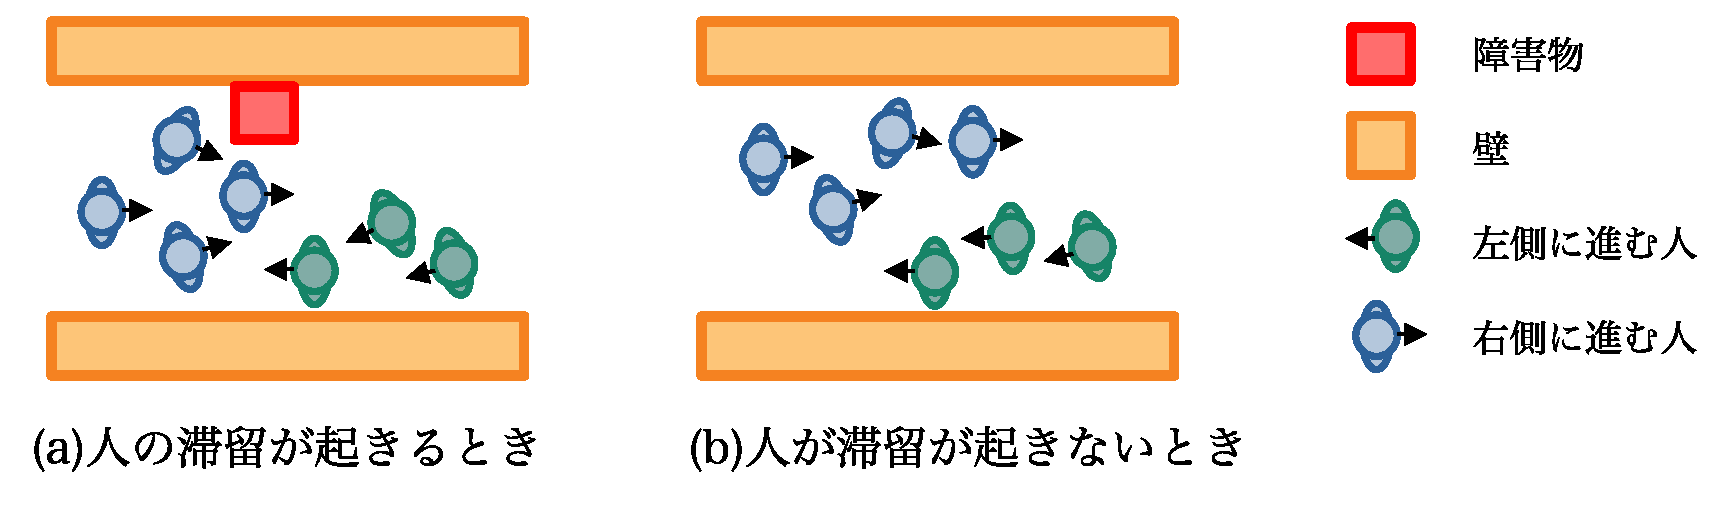
\includegraphics[width=14cm,clip]{figure/jinryu_image2_r2.eps}
     \caption{人流シミュレーションの活用例}
     \label{fig:jinryu_image}
    \end{center}
\end{figure}
%
%人流シミュレーションに必要な要素
人流シミュレーションを用いて人の動きを解析するためには,
人の動きを再現するための歩行者のモデル化(歩行者モデル)が必要である.
歩行者モデルは,求められる解析精度や解析規模に応じて使い分ける必要があるため,
ネットワークモデルやセルオートマトン,SocialForceModel(SFM)などが提案されている.
本章では,各歩行者モデルの使用用途や利点,欠点を用いて各手法の立ち位置について
述べる.

\if 0
歩行者モデルは,歩行者の移動を決定するためのアルゴリズムである.
シミュレーション対象が海岸から近い都市や人口が多い都市などの道路上の人々の流れを解析するためには,
数千人から数万人の解析が可能なネットワークモデルが用いられる(参考文献).
また,シミュレーション対象が商業施設や駅構内などの施設上の人々を解析するためには,
フロアフィールドモデルやSFMが用いられる(参考文献).
\fi
\begin{figure}[t]

  \begin{center}
     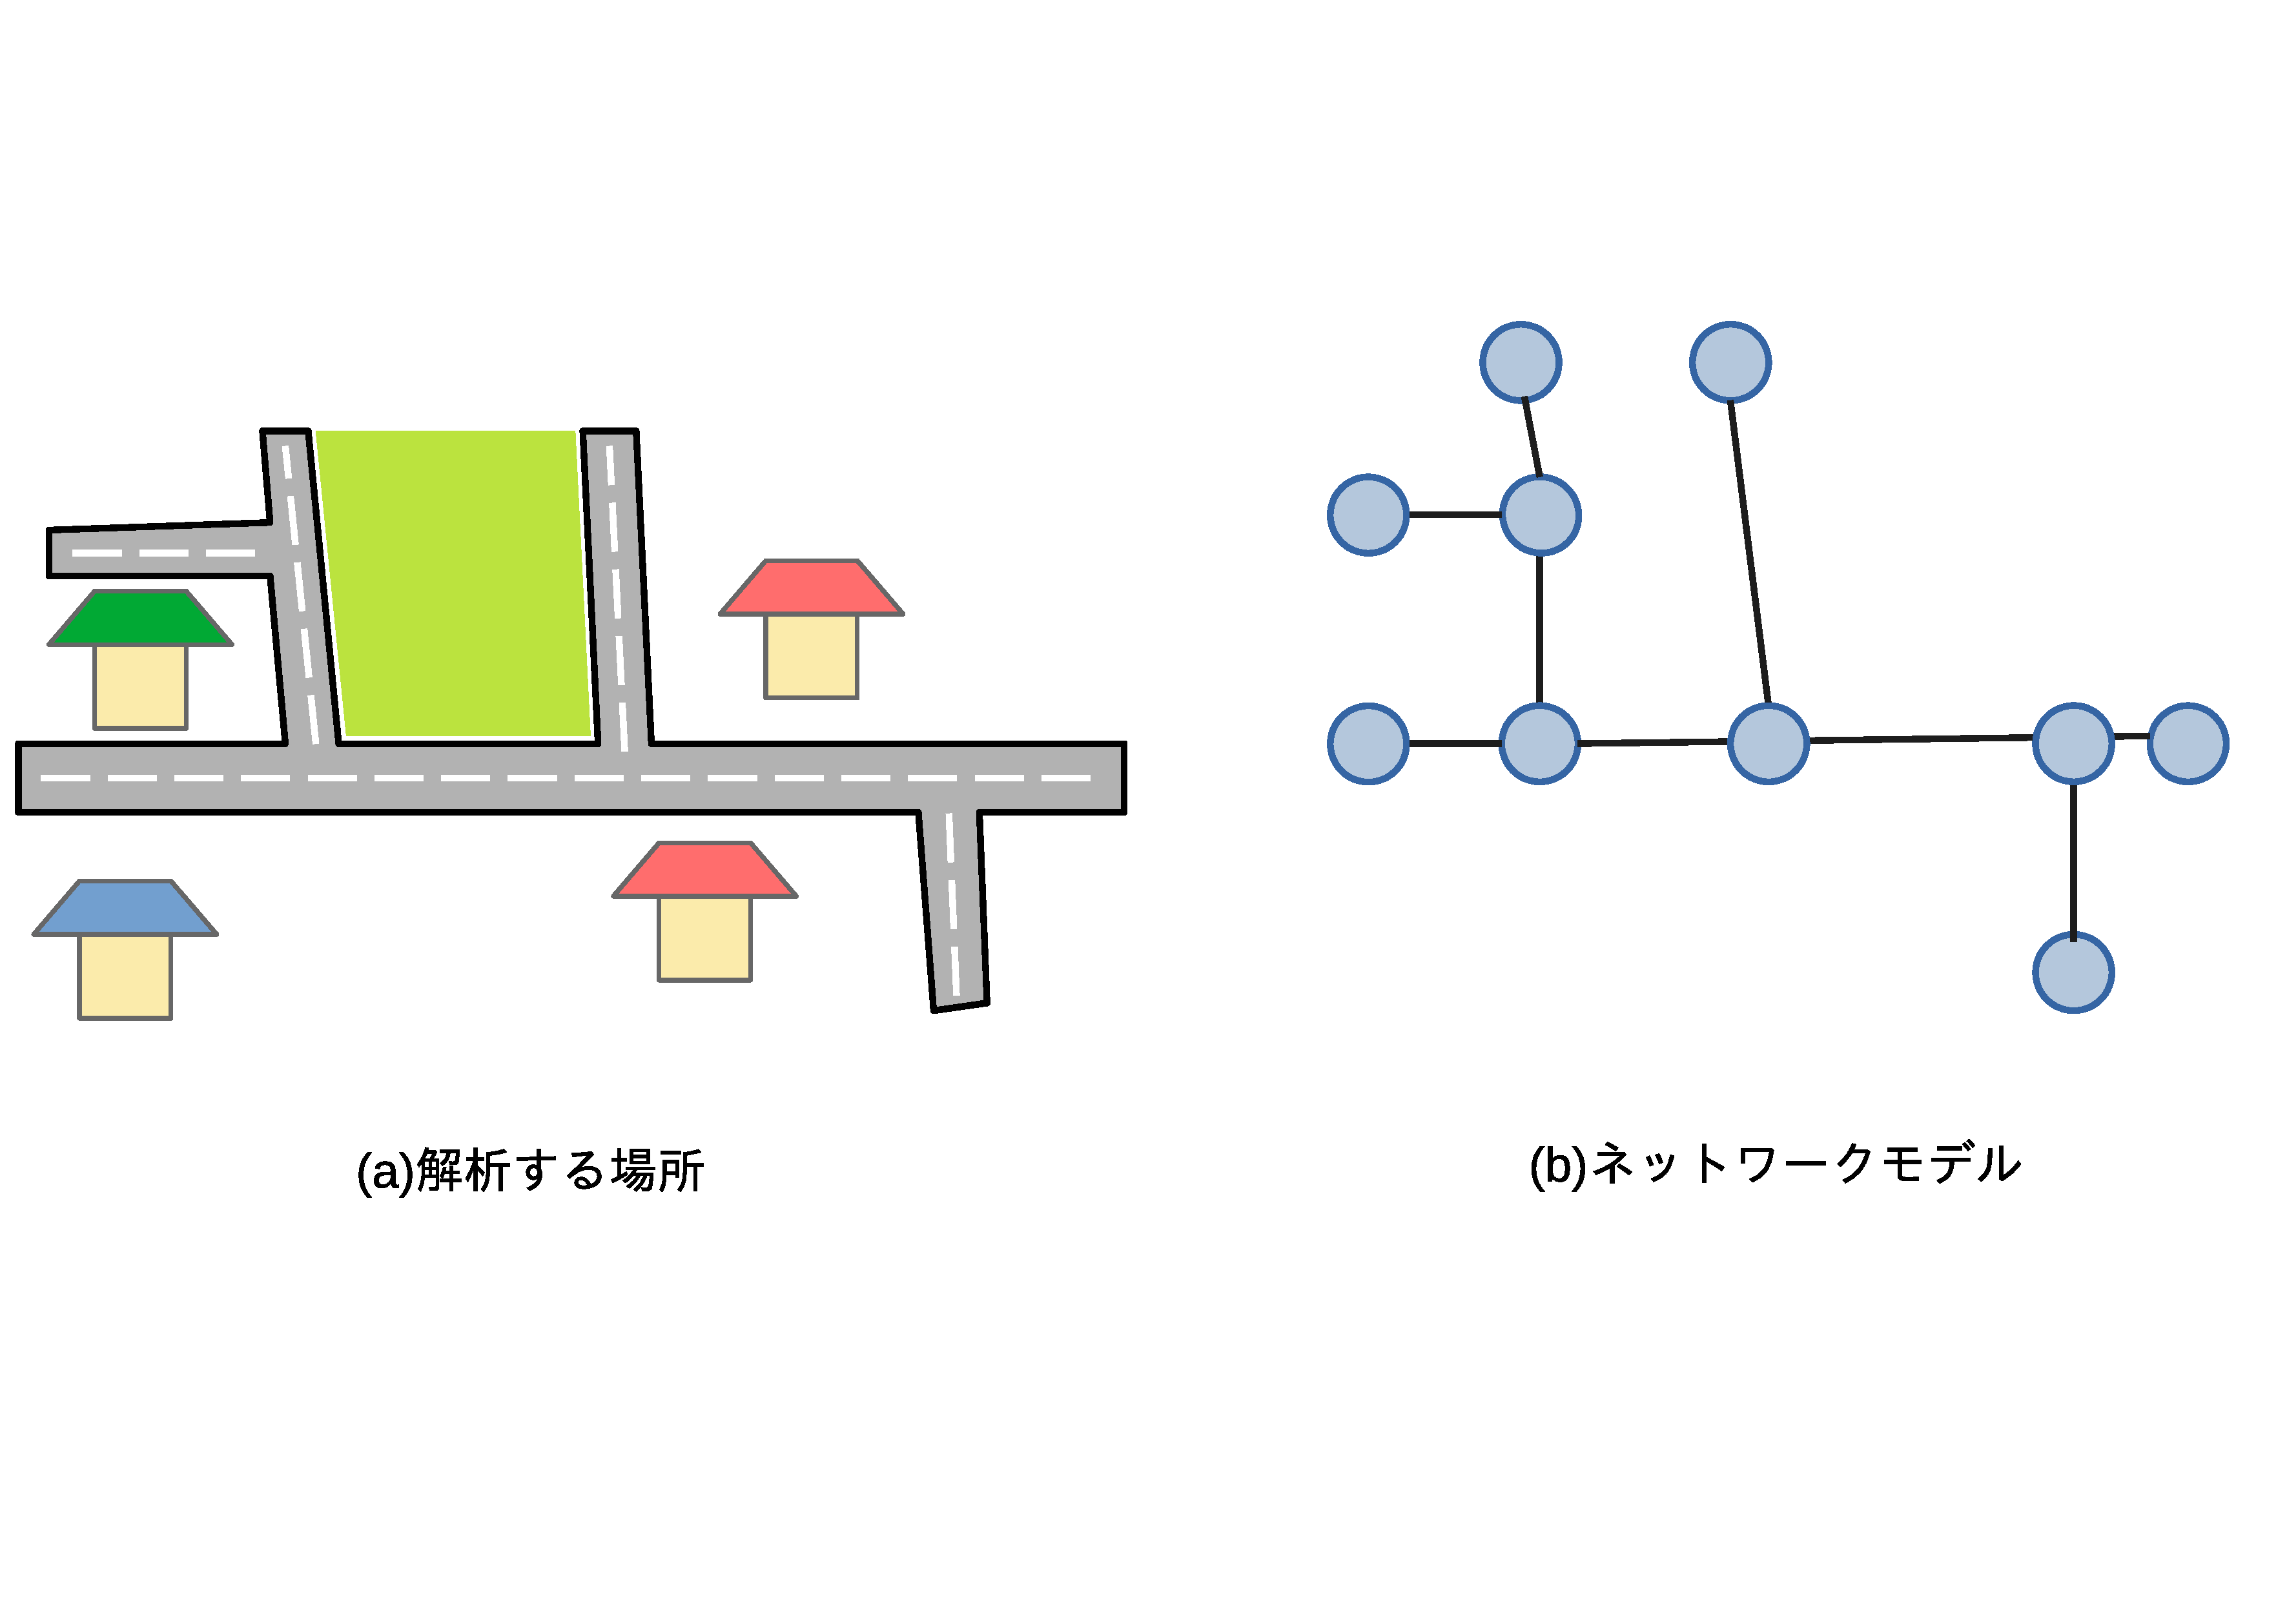
\includegraphics[width=13cm,clip]{figure/networkmodel_ex.eps}
     \caption{ネットワークモデルの例}
     \label{fig:network_ex}
    \end{center}
\end{figure}

\section{ネットワークモデル}
ネットワークモデルは,人々の移動や行動をネットワーク構造としてモデル化する手法である.
図\ref{fig:network_ex}にネットワークモデルの例を示す.
図\ref{fig:network_ex}中の(a)は解析対象であり,(b)はネットワークモデルである.
図\ref{fig:network_ex}中の(b)の青丸は交差点や道路の末端であり,ノードと呼ばれる.
ネットワークモデルでは,ノード間に数十から数百人単位で動かすことで,人の動きを解析する.
ネットワークモデルは,解析が高速であるが,モデルの準備に大きな作業が必要になるだけでなく,
モデルの定義に知識や経験が必要になることが多い.
ネットワークモデルを用いた解析では,都市間の人々の移動や,津波や地震などの
災害時における都市の避難シミュレーションのような解析人数が多い解析に用いられることが多い
(参考文献)
ネットワークモデルで建物内の人の流れを解析する場合は,図\ref{fig:nework_situnai}に示すように
解析領域内にメッシュ状にノードを配置することで解析できる(参考文献).
一方で,建物内などの避難シミュレーションでは,人の流量が低下する原因や滞留の原因を調査する
ことに用いられることが多いため,ネットワークモデルを用いた場合は,滞留などの再現ができない.
このため,人の流量が低下する原因や滞留の原因を突き止めるために解析するときは,静的フロアモデルやSFM
などが用いられることが一般的である.
%
%
\clearpage
\section{静的フロアモデル}
静的フロアモデルは,解析領域を格子状に分割し,

ーーーーーーーーーーーー下記は下書きーーーーーーーーーーー

静的フロアモデルは,図\ref{fig:serumaton}に示すようなフロアフィールドモデルの空間モデルを用いて
おり,格子ごとに目的地までの距離を設定し,確率を用いてエージェントを移動させることで解析する手法である.
図\ref{fig:huroa_model_image}に静的フロアフィールドモデルのイメージを示す.
図\ref{fig:huroa_model_image}中の格子は解析領域,青丸はエージェント,青色の矢印はエージェントの移動可能な
方向である.
図\ref{fig:huroa_model_image}のように,静的フロアフィールドモデルは,
図\ref{fig:huroa_manhattan}に室内からの退出時におけるマンハッタン距離を用いた
静的フロアフィールドの例を示す.
図\ref{fig:huroa_manhattan}中の格子は,各セルを示しており,セル中の数字は各セルの出口までの
マンハッタン距離を示す.

\doublefig{静的フロアフィールドモデルのイメージ}{floormodel_image}{5}{1.5}{マンハッタン距離を用いた静的フロアフィールドモデルの例}{floormodel_kyori}{5}

%\doublefig{マンハッタン距離を用いた静的フロアフィールドモデルの例}{}{5}{1.5}{静的フロアフィールドモデルを用いたアーチ現象の再現}{floormodel_ex2}{5}

\begin{figure}[t]
	\begin{minipage}[b]{0.45\linewidth}
		\centering
		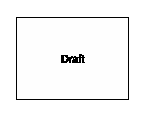
\includegraphics[keepaspectratio, scale=2.5]{figure/draft.eps}
		\caption{アーチ現象の例}
		\label{fig:a-tigenshou}
	\end{minipage}
	\begin{minipage}[b]{0.45\linewidth}
		\centering
		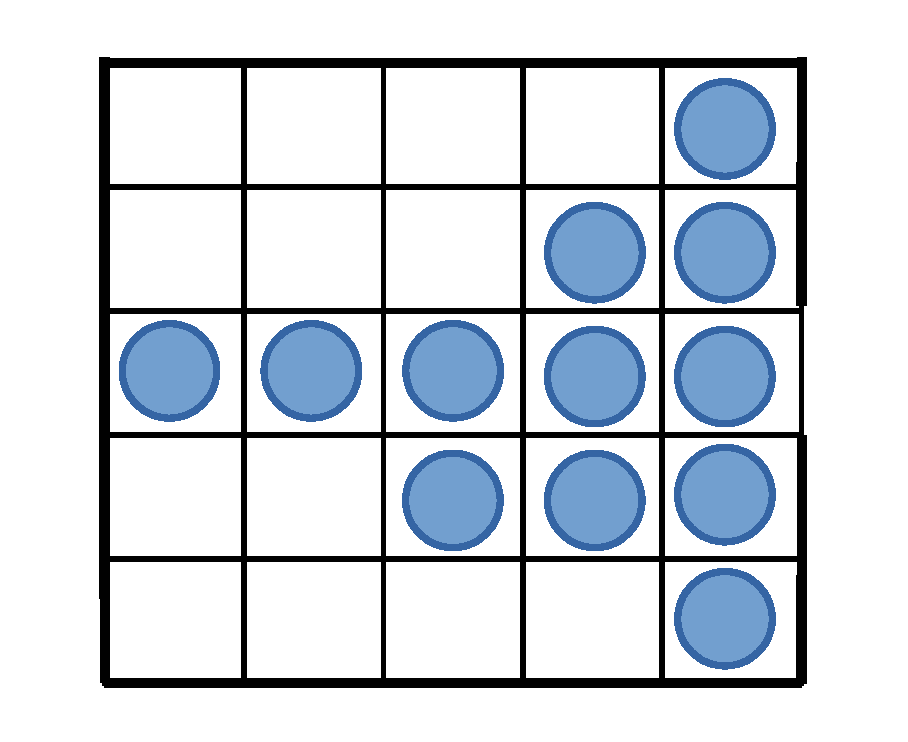
\includegraphics[keepaspectratio, scale=0.35]{figure/floormodel_ex2.eps}
		\caption{静的フロアフィールドモデルを用いたアーチ現象}
		\label{fig:floormodel_ex2}
	\end{minipage}
\end{figure}


静的フロアフィールドモデルは,図\ref{fig:huroa_manhattan}に示すように,計算対象のエージェントの周囲のセルのなかから,出口までの
距離が小さくなるようなセルを選択することで,出口までの解析が可能となる.
静的フロアフィールドモデルの利点は,解析前に各格子の計算を事前にできるため,非常に高速な
解析が可能である点である.
一方で,静的フロアフィールドは,出口前に形成されるアーチ現象の再現度が低いことが知られている.
図\ref{fig:huroa_model_ketten}に静的フロアフィールドモデルを用いた場合の出口前に形成される
アーチ現象の例を示す.
図\ref{fig:huroa_model_ketten}中の~~~である.
静的フロアフィールドモデルは,図\ref{fig;ruroa_model_ketten}のように,格子に一人のみ入ることができる
ことから,動きが格子サイズに制約されるため,出口付近の再現度が低い.
フロアフィールドモデルを用いた解析では,〇〇や△△,□□を用いることで,解析精度の向上が行われている
が,格子サイズの成約から,精度の向上に上限がある.
このため,高い解析精度が必要な場合は,SocialForceMoel(SFM)のような
解析領域を連続座標で解析する手法が用いられることが多い

\begin{figure}[htbp]
  \begin{minipage}[b]{0.5\linewidth}
    \centering
    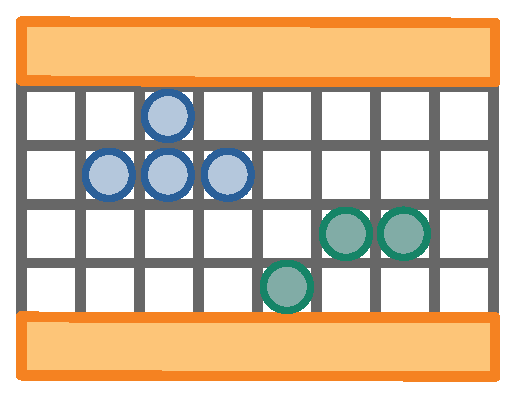
\includegraphics[keepaspectratio, scale=0.37]{figure/seruotomaton_image4.eps}
    \caption{フロアフィールドモデルの例}
    \label{fig:serumaton}
  \end{minipage}
  \begin{minipage}[b]{0.5\linewidth}
    \centering
    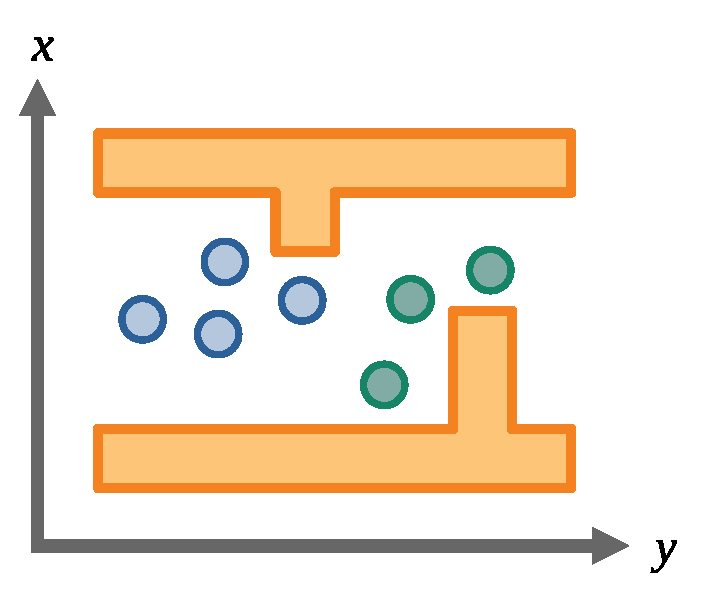
\includegraphics[keepaspectratio, scale=0.37]{figure/renzoku_image2.eps}
    \caption{二次元連続座標モデルの例}
    \label{fig:renzoku}
  \end{minipage}
\end{figure}



\section{SocialForceModel(SFM)}
SFMは,人間の社会心理学的な要素と物理的な力を結びつけた動力学モデルであり,
近傍のエージェントや壁といった障害物から受ける力によってエージェントの進行方向
や速度を解く.本手法は,心理的変数が組み込まれているため,災害時の避難シミュ
レーションによく用いられる\cite{21_Isozaki}\cite{ando_sfm}.

%\section{仮)SFMの解析空間}
SFMの解析空間は,二次元
連続空間モデルが用いられる.二次元連続空間モデルは,解析領域を分割せずに$(x,y)$の連続した座標で
解析する手法である.図\ref{fig:renzoku}に図\ref{fig:jinryu_image2}の例を二次元連続座標で
考えた例を示す.図\ref{fig:renzoku}中の矢印は座標の$x$と$y$を示している.SFMは,
図\ref{fig:serumaton}のフロアフィールドモデルのように格子上のエージェント数に制限がなく,
エージェントの位置を座標で考えるため,人流の再現度が高い.
%\section{仮)SFMにおけるエージェント移動}
SFMにおけるエージェント移動は,目的地へ進む力と他のエージェントから受ける力,
壁などの障害物から受ける力を用いる運動方程式を用いて求める.
式(\ref{eq:sfm_siki1})にSFMの運動方程式を示す.
%
\begin{eqnarray}
 m_i \frac{dv_i}{dt} = m_i \frac{v_i^0(t)e_i^0(t)-v_i(t)}{t_i}
 +\sum_{j(\neq i)}f_{ij}+\sum_{W}f_{iW}
 \label{eq:sfm_siki1}
\end{eqnarray}
%
式(\ref{eq:sfm_siki1})中の
総和の記号$\sum_{j(\neq i)}f_{ij}$は,エージェント$i$以外のすべ
てのエージェント$j$の総和をとることを意味する.同様に,$\sum_{W}f_{iW}$
は,すべての壁$W$の総和をとることを意味する.式
(\ref{eq:sfm_siki1})中の$m_i$はエージェント$i$の体重,$v_i^0(t)$はエージェ
ントの希望速度,$e_i^0(t)$は,目的地までの単位ベクトル,$v_i(t)$
は現在の速度ベクトル,$t_i$は時定数である.式(\ref{eq:sfm_siki1})の第一
項はエージェントが目的地へ進む力,第二項は他のエージェントから受ける力
$f_{ij}$,第三項は壁などの障害物から受ける力$f_{iW}$の合力である.
$f_{ij}$と$f_{iW}$は,式(\ref{eq:sfm_siki2})と式(\ref{eq:sfm_siki3})を用
いて導出する.
%
\begin{eqnarray}
 f_{ij} = & \{A_i exp[\frac{r_{ij} - d_{ij}}{B_i}]
  + kg(r_{ij} - d_{ij})\} n_{ij}
+ \kappa g (r_{ij} - d_{ij}) \Delta
  v^t_{ij} t_{ij}
 \label{eq:sfm_siki2}
\end{eqnarray}
%
\begin{eqnarray}
 f_{iW} = \{A_i exp[\frac{r_{i} - d_{iW}}{B_i}]
  + kg(r_{i} - d_{iW})\} n_{iW} + \kappa g (r_{i} - d_{iW})
  (v_i t_{iW}) t_{iW}
 \label{eq:sfm_siki3}
\end{eqnarray}
%
表\ref{tab:tab_para}に
式(\ref{eq:sfm_siki2}),(\ref{eq:sfm_siki3})中の変数を示す.
衝突時関数$g(x)$はエージェント同士や壁などに衝突したときに値をとる関数
である.式(\ref{eq:gx_siki})に衝突時関数$g(x)$の条件式を示す.
%
\begin{equation}
  \label{eq:gx_siki}
  g(x) =
  \begin{cases}
    1 & (x<0) \\
    0 & otherwise
  \end{cases}
\end{equation}
%
SFMの衝突時の計算は,条件式である式(\ref{eq:gx_siki})を用いることで,衝突時のみ計算できる.
SFMを用いる人流シミュレーションのフローチャートを図
\ref{fig:sfm_flowchart}に示す.
図\ref{fig:sfm_flowchart} 中の目的地へ進む力の計算は,式(\ref{eq:sfm_siki1})中の第一項を
用いて算出する.また,他のエージェントから受ける力の計算は,式(\ref{eq:sfm_siki2})を用いて
算出する.そして,壁などの障害物から受ける力の計算は,式(\ref{eq:sfm_siki3})を用いて算出する.
SFMを用いた人流シミュレーションは,図\ref{fig:sfm_flowchart}に示すように,
式(\ref{eq:sfm_siki1})の運動方程式を積分することで,新しい時間のエージェントの位置と速度を求
めることができる.


\begin{table}[hbtp]
 \begin{center}
  \caption{SFMのパラメータ}
    \begin{tabular}{c|c}
     \hline \hline
     $d_{ij}$ & エージェント間の距離 \\
     \hline
     $t_{ij}$ & エージェント$i$とエージェント$j$の衝突面の垂直ベクトル \\
     \hline
     $n_{ij}$ & エージェント$i$とエージェント$j$の衝突面の法線ベクトル\\
     \hline
     $r_i$ & エージェント$i$の体の半径 \\
     \hline
     $r_{ij}$ & エージェント$i$とエージェント$j$の体の半径の和 \\
     \hline
     $t_{iW}$ & エージェント$i$と壁$W$の衝突面の垂直ベクトル\\
     \hline
     $n_{iW}$ & エージェント$i$とエージェント$W$の衝突面の法線ベクトル \\
     \hline
     $A_i$ & エージェント$i$のインタラクション作用 \\
     \hline
     $B_i$ & エージェント$i$の反発作用 \\
     \hline
     $k$ & 衝突時の反発力係数\\
     \hline
     $\kappa$ & 衝突時の摩擦力係数 \\
     \hline
     $\Delta v_{ij}$ & エージェント$i$とエージェント$j$の接線速度の差 \\
     \hline
     $g(x)$ & 衝突時関数 \\
     \hline
    \end{tabular}
  \label{tab:tab_para}
 \end{center}
\end{table}

\begin{figure}[hbtp]
 \begin{center}
  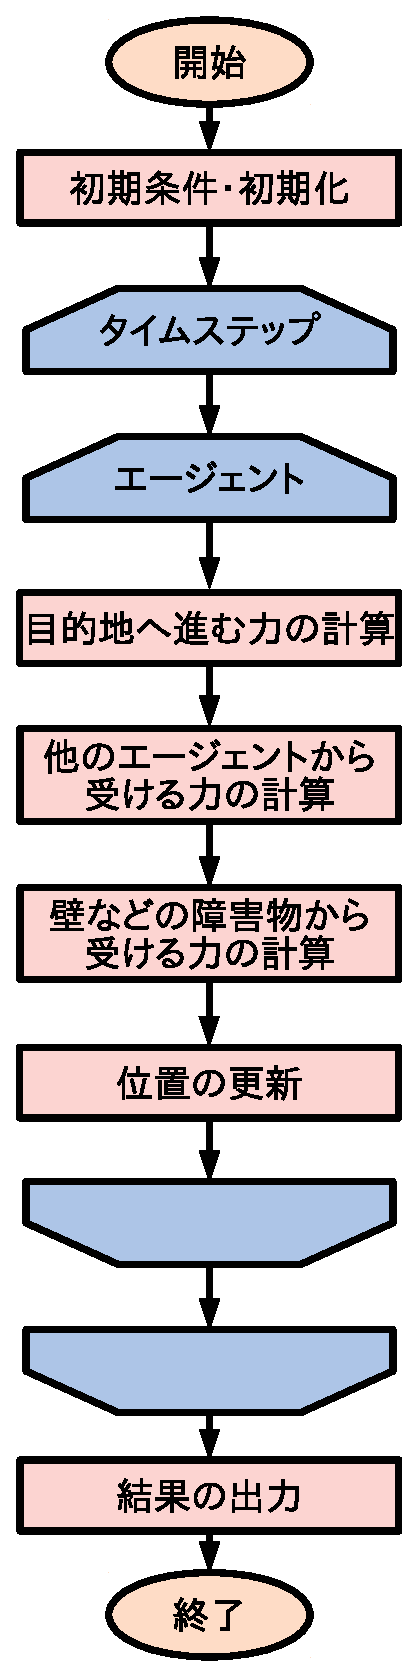
\includegraphics[width=4cm,clip]{figure/sfm_flowchart.eps}
  \caption{SFMを用いた人流シミュレーションのフローチャート}
  \label{fig:sfm_flowchart}
 \end{center}
\end{figure}


\newpage
\subsection{周囲のエージェントから受ける力}
他のエージェントから受ける力は,解析領域全体に存在する他のエージェントから
受ける.このため,SFMは,解析する人数が増えると他のエージェントから受ける
力の計算時間が長くなる.他のエージェントから受
ける力の計算負荷を削減するために,SFMを用いる人流シミュレーションでは,
他のエージェントから受ける力を計算する範囲を限定することが多い
\cite{seru_sfm1}\cite{seru_sfm2}.
他のエージェントから受ける力を計算する範囲を限定することで,遠くに存在する
エージェントから受ける力を0に近似することができる.
%
\begin{figure}[t]
 \begin{center}
  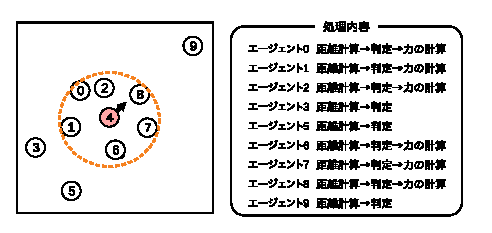
\includegraphics[width=11.5cm,clip]{figure/eikyo_hankei_ex1.eps}
  \caption{他のエージェントから受ける力の範囲を限定するときの例}
  \label{fig:sougo_hani}
 \end{center}
\end{figure}
%
\begin{figure}[t]
 \begin{center}
  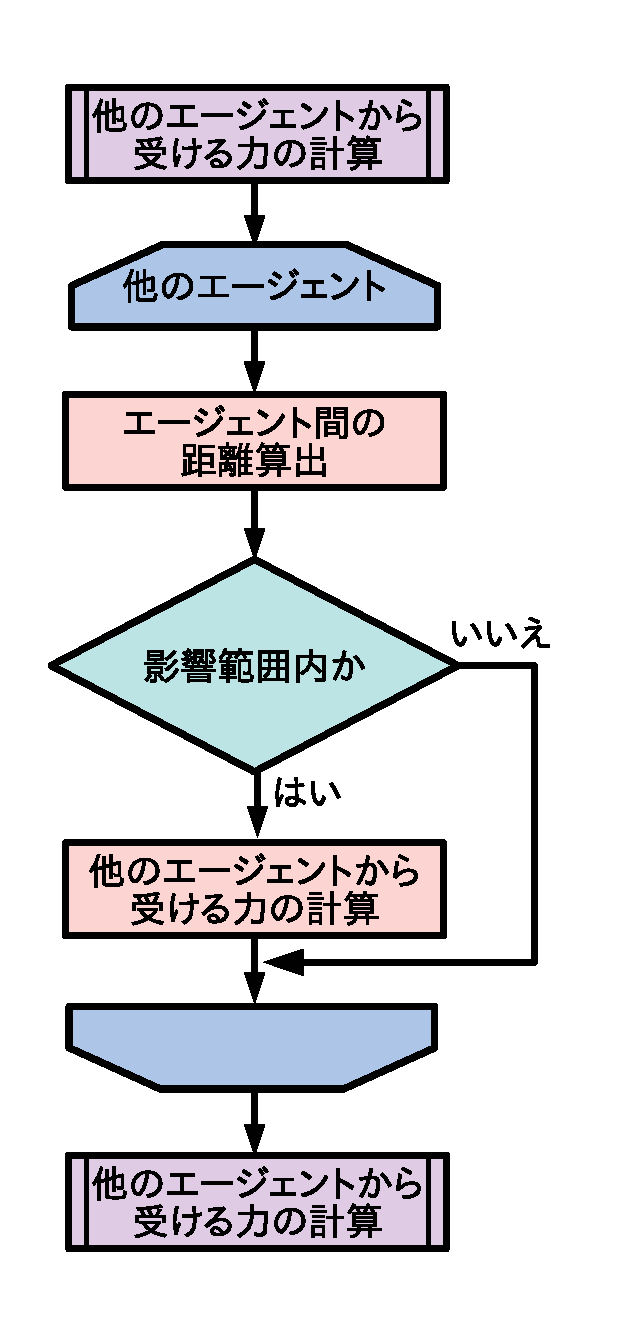
\includegraphics[width=5cm,clip]{figure/agent_flow.eps}
  \caption{SFMにおける周囲のエージェントから受ける力の計算}
  \label{fig:sougo_hani_flow}
 \end{center}
\end{figure}
%
図\ref{fig:sougo_hani}に他のエージェントから受ける力の計算範囲の例
を示す.図\ref{fig:sougo_hani}の赤丸は他のエージェントから受ける力を計算
するエージェント,黒丸はエージェント4が計算するときの他のエージェント,
オレンジ色の点線は他のエージェント
から受ける力の範囲を示す.図\ref{fig:sougo_hani} のエージェント4は,
オレンジ色の点線内に存在するエージェント0,1,2,6,7,10の合計5人から力を
受ける.本論文では,近くのエージェントから受ける力の範囲を限定するSFMを前提
として述べる.
近くのエージェントから受ける力の範囲は,図\ref{fig:sougo_hani}の
ように,計算するエージェントの半径数メートルの範囲である.このため,SFMでは,
他のエージェントが近くのエージェントから受ける力の範囲に存在するか判定が必要
である.
この範囲に存在するかの判定は,エージェント$i$とエージェント$j$とのエージェン
ト間の距離$d_{ij}$の算出が必要である.
本論文では,式(\ref{eq:kyori_siki})を用いてエージェント間の距離$d_{ij}$
を求め,他のエージェントから受ける力の範囲内であるかどうか判定する.
%
\begin{eqnarray}
 d_{ij} =  \sqrt{ (x_i-x_j)^2 + (y_i-y_j)^2 }
 \label{eq:kyori_siki}
\end{eqnarray}
%
式(\ref{eq:kyori_siki})中の$x_i$と$y_i$はエージェント$i$の座標$(x_i,y_i)$,$x_j$
と$y_j$はエージェント$j$の座標$(x_j,y_j)$である.エージェント$i$は
,式(\ref{eq:kyori_siki})
で求めたエージェント距離$d_ij$が他のエージェントから受ける力の範囲内であれば,
エージェント$j$から式(\ref{eq:sfm_siki2})を用いて算出した力を受ける.
他のエージェントから受ける力の範囲の半径を$R$としたとき,エージェント$i$の他のエージェント
$j$が範囲内にいるかどうかの判定式を式(\ref{eq:jouken_siki1})に示す.
%
\begin{eqnarray}
  \label{eq:jouken_siki1}
  R \geq d_{ij}
\end{eqnarray}
%
エージェント$i$は,式(\ref{eq:jouken_siki1})の条件を満たす他のエージェント$j$から式(\ref{eq:sfm_siki2})
で求まる力を受ける.
他のエージェントから受ける力の範囲を限定するSFMのフローチャート
を図\ref{fig:sougo_hani_flow}に示す.
図\ref{fig:sougo_hani_flow}のフローチャートでは,各エージェントに対しエー
ジェント間の距離を計算し,範囲内であるか判定することで,他のエージェントから受ける力の範囲を限定
する.



\clearpage
\subsection{周囲の壁から受ける力}
周囲の壁から受ける力は,エージェントの周囲の障害物を避けるために受ける力である.
SFMを用いた人流シミュレーションは,壁や机などの障害物を粒子として計算することが
一般的である(参考文献).
図\ref{fig:kaberyuusi_ex}に壁を粒子化した例を示す.
図\ref{fig:kaberyuusi_ex}中の緑色の丸はエージェント,黄色の丸は壁粒子である.
図\ref{fig:kaberyuusi_ex}のように,障害物を粒子化して解析する場合は,
机や壁などの障害物を粒子のかたまりとして離散化する.
エージェントは,影響範囲に存在する各粒子から力を受ける.
このため,
エージェントの周囲の障害物を避ける力は,
障害物の粒子の増加に応じて障害物を避ける力の計算回数が増加する
傾向がある.
\figref{fig:kabe_flowchart}に周囲の壁粒子から受ける力の計算するフローチャートを示す.
\figref{fig:kabe_flowchart}に示すように,壁粒子から受ける力の計算は,
計算対象であるエージェン$i$と壁粒子の中心座標間の距離$d_{iW}$が影響範囲内であれば,
エージェント$i$が受ける力を算出する.


\begin{figure}[t]
 \begin{center}
  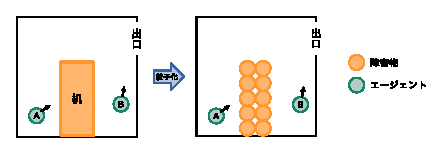
\includegraphics[width=11.5cm,clip]{figure/shougaibutu_ryuusika.eps}
  \caption{障害物を粒子として計算する例}
  \label{fig:kaberyuusi_ex}
 \end{center}
\end{figure}


\begin{figure}[t]
 \begin{center}
  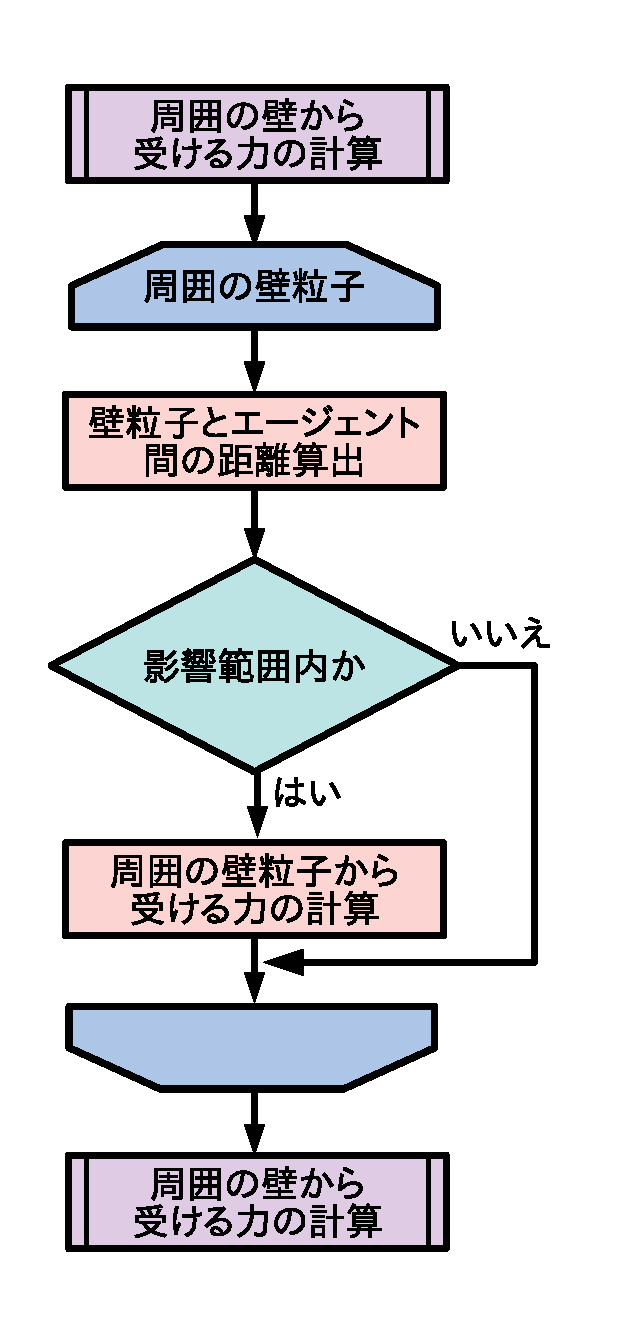
\includegraphics[width=5cm,clip]{figure/kabe_flow.eps}
  \caption{周囲の壁から受ける力の計算のフローチャート}
  \label{fig:kabe_flowchart}
 \end{center}
\end{figure}

\newpage
\subsection{経由地の設定}
%経由地のことを述べる
SFMは,エージェントと目的地の間に障害物が存在するとスタック現象が発生することが
報告されている(参考文献).
スタック現象は,エージェントが動かなくなる現象のことであり,障害物から受ける力と
目的地に向かう力の関係により生じる.
図\ref{fig:sutakku_ex}にSFMでスタック現象が生じる例を示す.
図\ref{fig:sutakku_ex}中の緑色の丸はエージェント,矢印はエージェントの進行方向,
オレンジ色の四角は机などの障害物である.
図\ref{fig:sutakku_ex}中のエージェントAとエージェントBは解析領域右上の出口に向かうため,
エージェントAが机などの障害物に向かって進む.
この場合は,エージェントAが机に向かって進み続けることや机の上を歩くなどの
想定しない動きをすることがある.
このため,障害物が多く存在するような解析では,出口(目的地)だけでなく,
目的地までの道のりを示す経由地を設定することで,エージェントのスタック現象や
想定しない動きを防ぐことができる.
図\ref{fig:keiyuti_ex}に経由地を設定する例を示す.
図\ref{fig:keiyuti_ex}中の緑色の丸はエージェント,四角は障害物,青色の四角は経由地,
赤色の四角は目的地を示す.
図\ref{fig:keiyuti_ex}の例では,エージェントAは,経由地を通ったあとに目的地に進むため,
図\ref{fig:sutakku_ex}のように机に進むことが防げる.
教室などの障害物多い解析では,
図\ref{fig:jitumondai_ex}に示すように,複数の経由地を設定する必要がある.
図\ref{fig:jitumondai_ex}の例では,エージェントは一番近くの経由地から
目的地までの道のりを辿る.
目的地までの道のりを決定する手法は,ダイクストラ法などのグラフ理論で用いられる
手法が使われることが多い\cite{keiro_daikusu}\cite{sfm_with_daikusutora}.

\begin{figure}[t]
 \begin{center}
  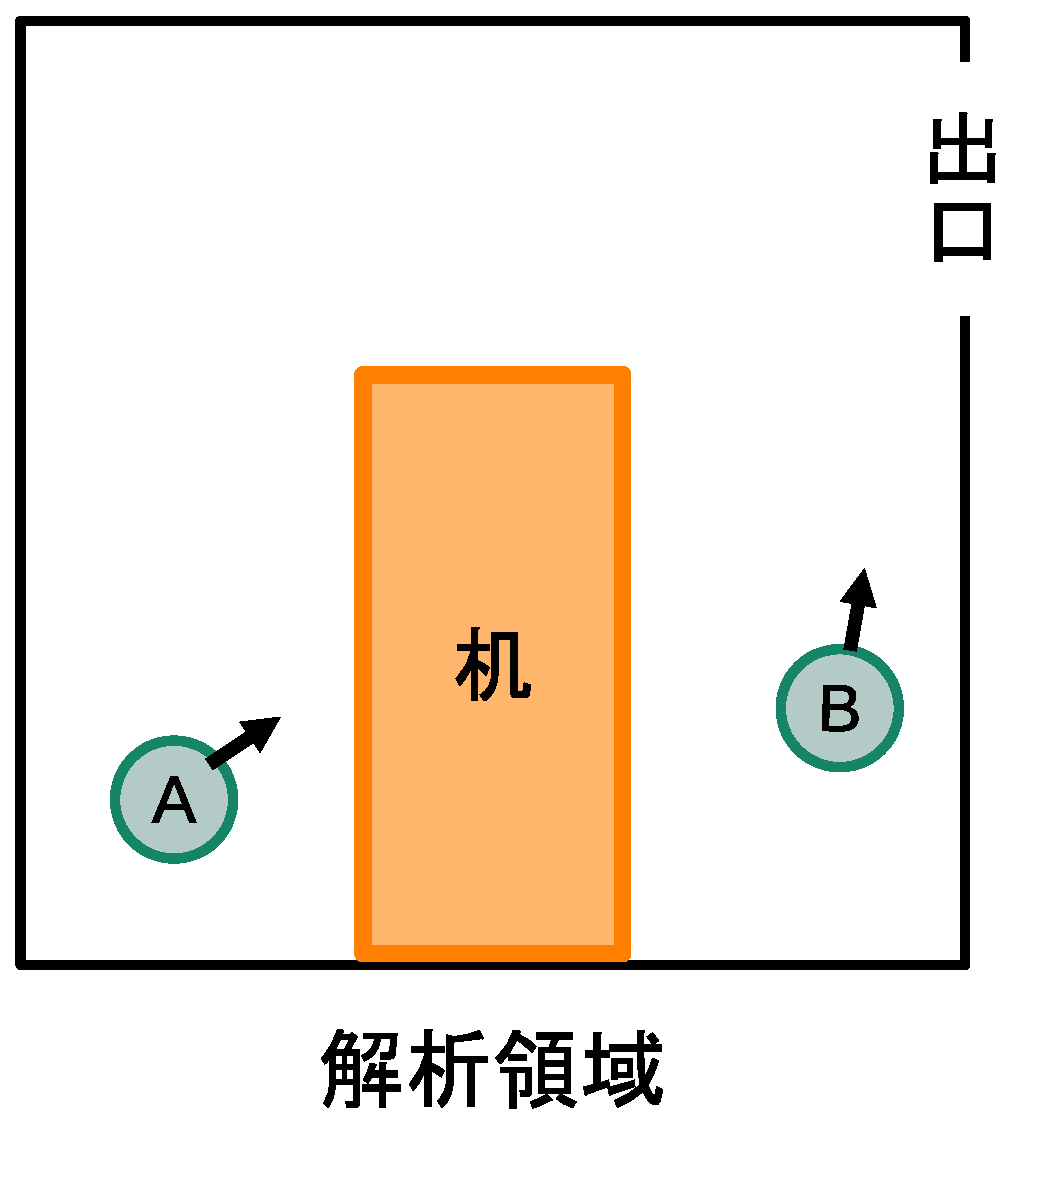
\includegraphics[height=4cm,clip]{figure/sutakku_ex.eps}
  \caption{SFMでスタック現象が起きる例}
  \label{fig:sutakku_ex}
 \end{center}
\end{figure}

\begin{figure}[t]
 \begin{center}
  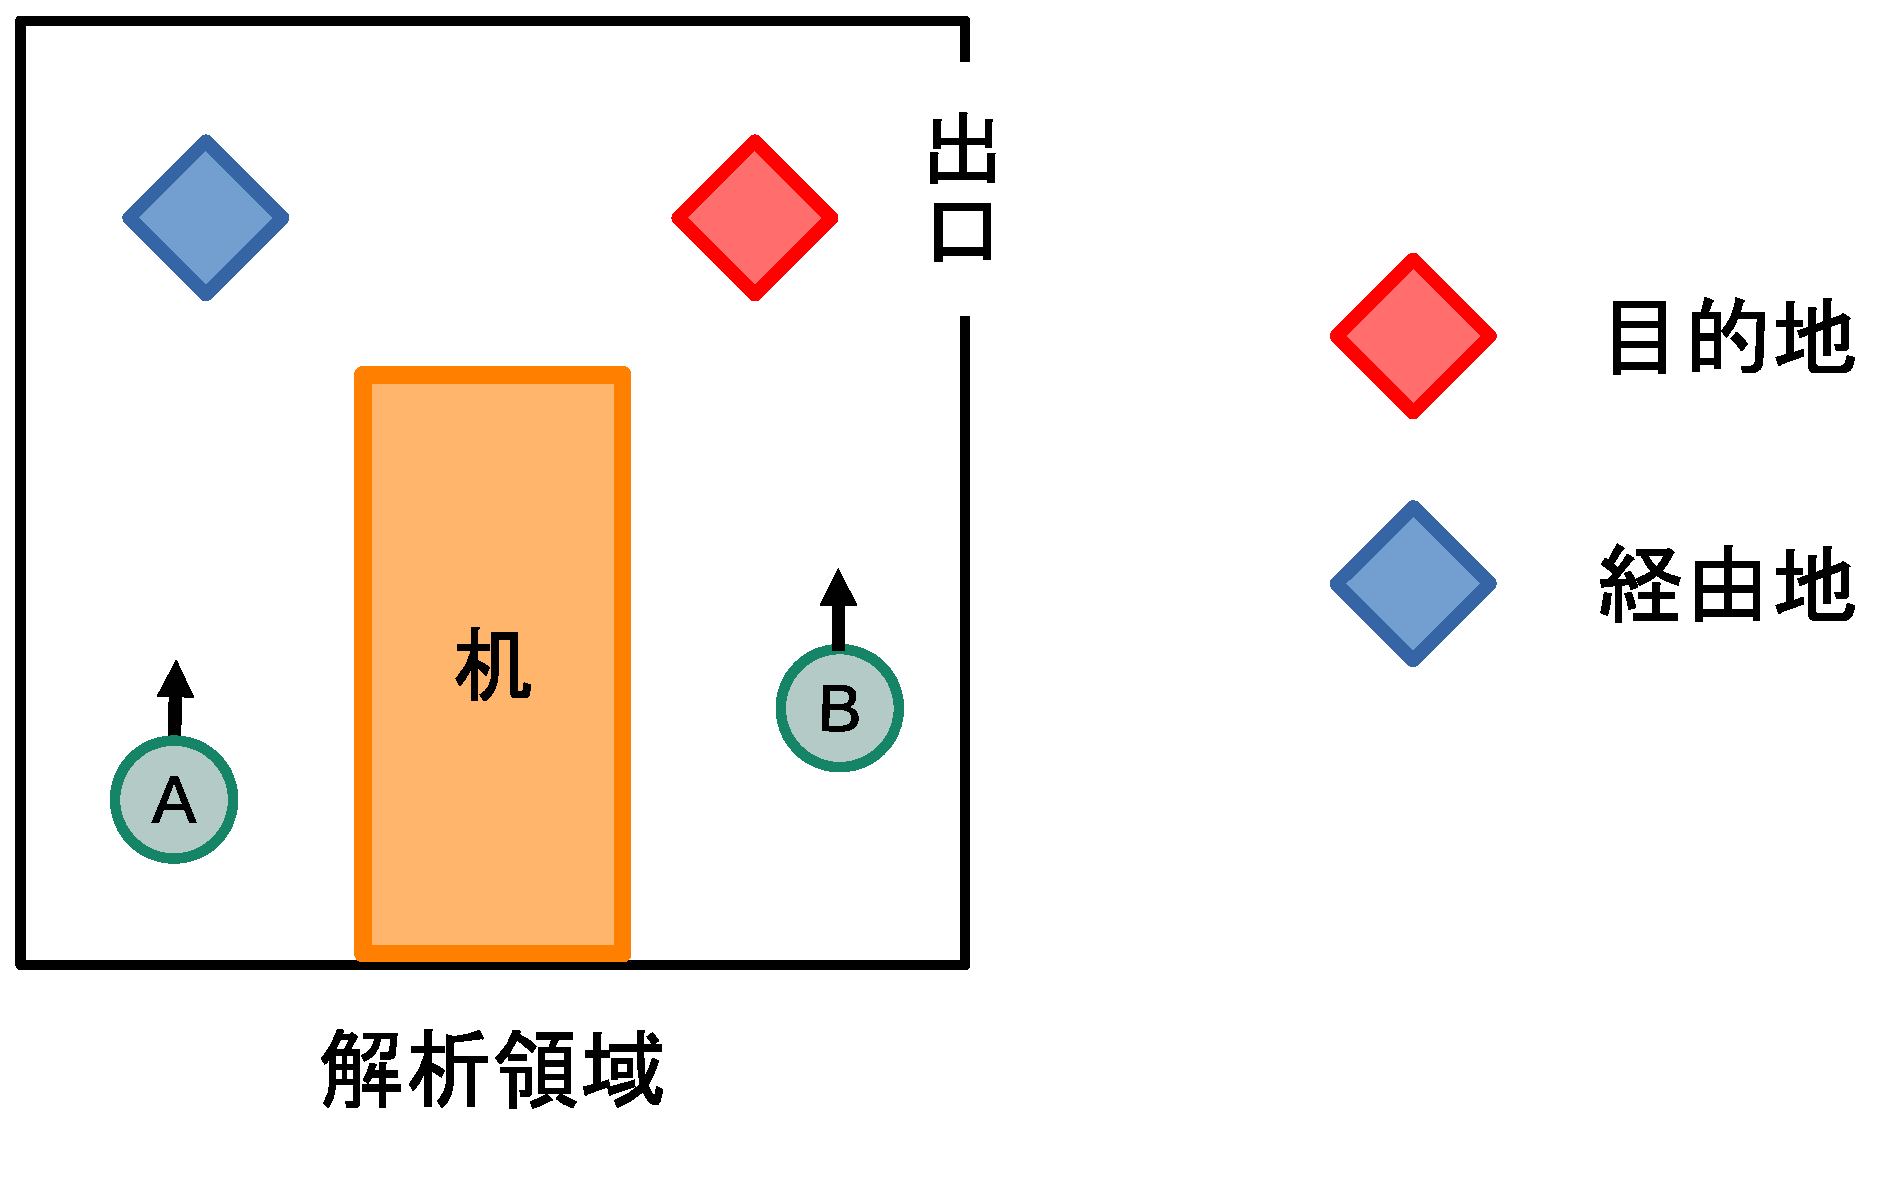
\includegraphics[height=4cm,clip]{figure/keiyuti_ex.eps}
  \caption{経由地を設定するSFMの例}
  \label{fig:keiyuti_ex}
 \end{center}
\end{figure}

\begin{figure}[t]
 \begin{center}
  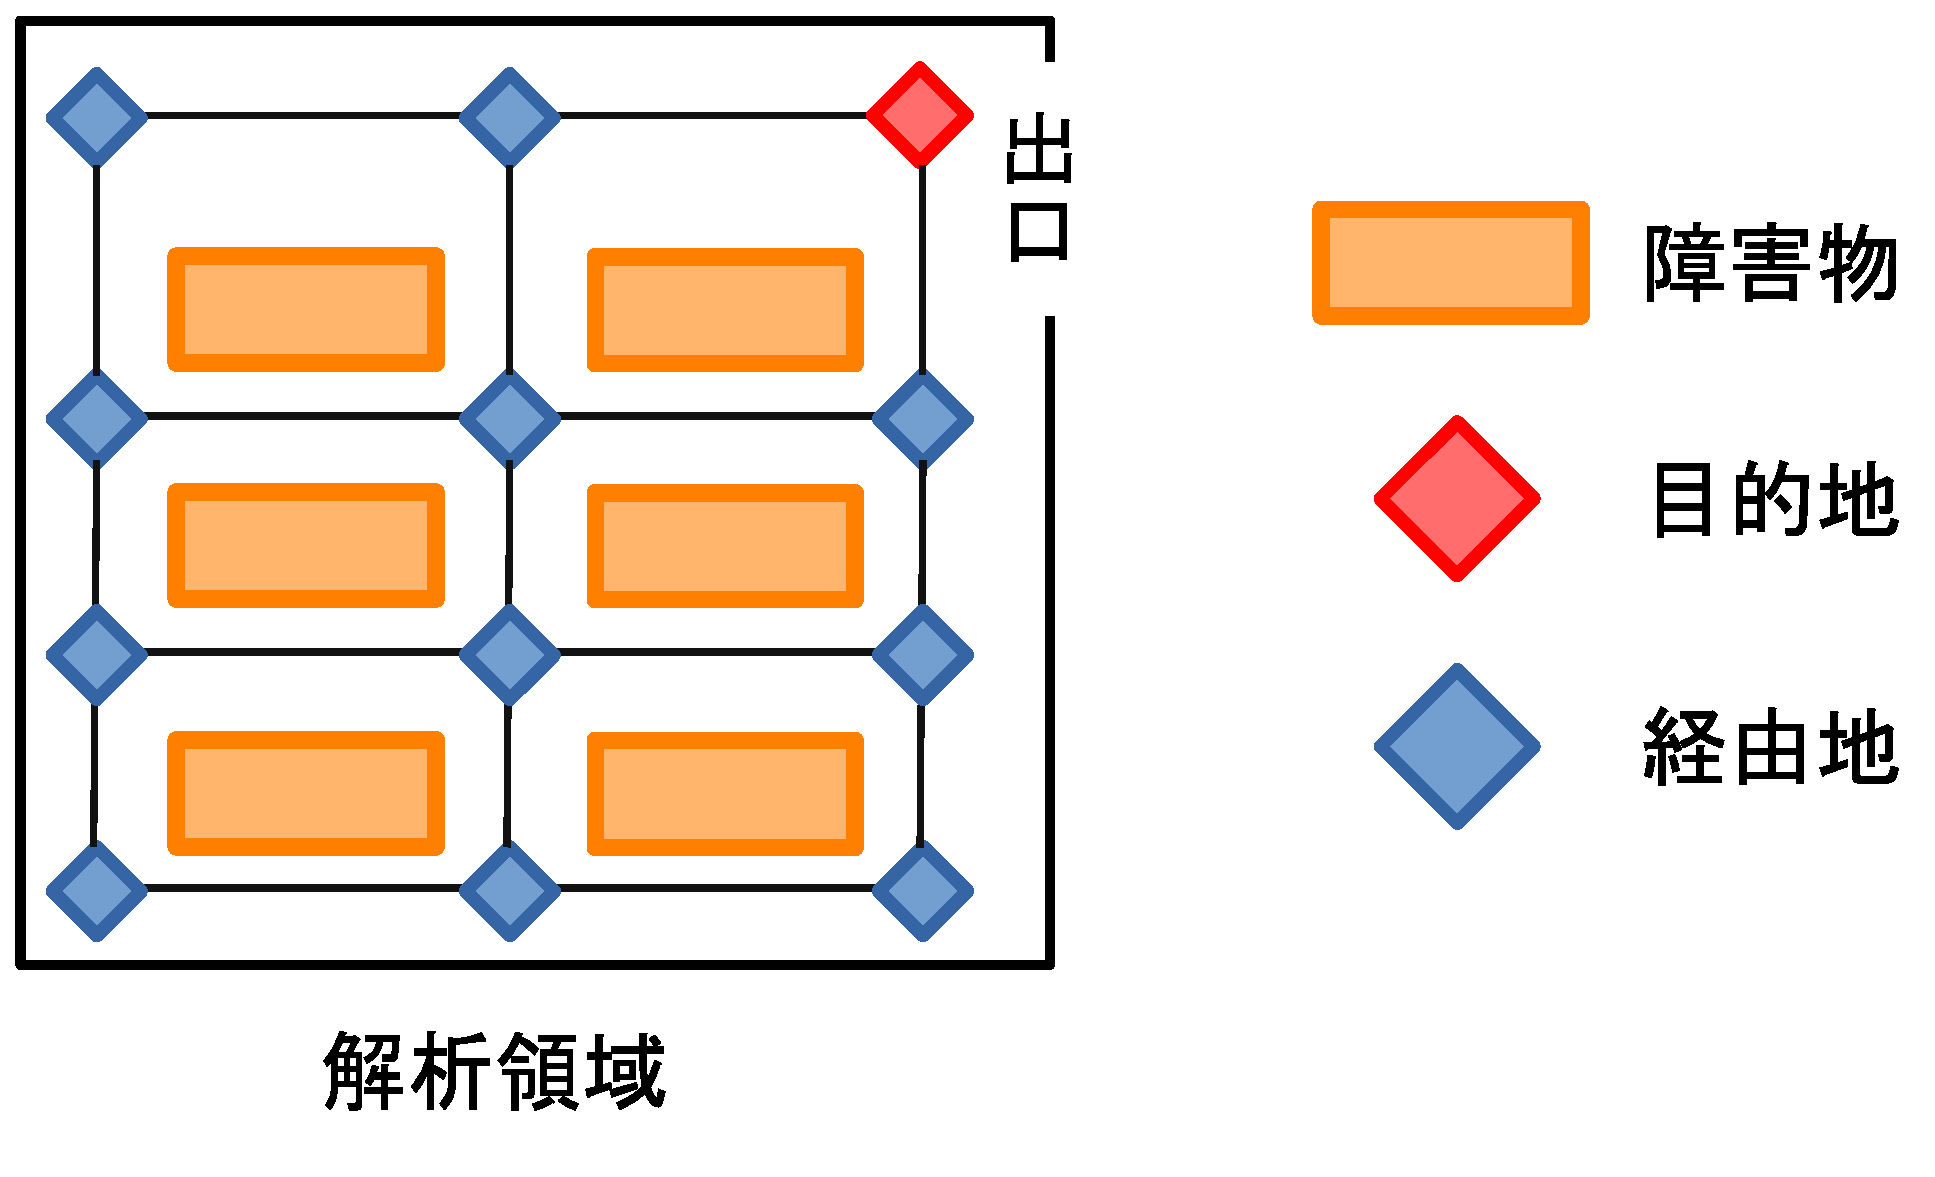
\includegraphics[height=4cm,clip]{figure/keiyuti_ex2.eps}
  \caption{教室からの避難シミュレーションにおける経由地の設定}
  \label{fig:jitumondai_ex}
 \end{center}
\end{figure}

\subsection{視野のパラメータ}
SFMは,視野(参考文献)やグループ特性,車椅子などといった
解析対象に応じてパラメータを組み込むことが可能である.
SFMの追加できるパラメータのなかでも,視野パラメータは,人間の視野を再現できること
から幅広く利用されている(参考文献).
視野を用いたSFMは,エージェントの影響範囲を扇状の範囲に限定することで,
人間の視野を再現できる.
\figref{fig:siya_hani}に視野を用いたSFMの影響範囲の例を示す.
\figref{fig:siya_hani}中の白色の丸はエージェント,白色の丸の数字はエージェント番号,
黒色の矢印はエージェント4の進行方向,緑色の範囲はエージェント4の影響範囲,
オレンジ色の丸は従来のSFMの影響範囲を示す.
\figref{fig:siya_hani}に示すように,エージェント4は,影響範囲が緑色の視野範囲に
存在するエージェント2,8から力を受ける.
周囲のエージェントが視野範囲に存在するかの判定は,エージェント間の距離$d_{ij}$と
エージェント間の角度の計算が必要となる.
エージェント間の距離$d_{ij}$は,式\eqref{eq:kyori_siki}を用いて算出する.
エージェント間の角度は,エージェント$i$の座標,エージェント$i$の進行方向ベクトル$e$,
エージェント$j$の座標の3点のなす角$\theta_{ij}$である.
3点のなす角$\theta_{ij}$が視野角$\frac{1}{2}\theta_{view}$以下かつエージェント間距離$d_{ij}$
が影響半径$R$以下である条件を満たす場合は,周囲のエージェント$j$がエージェント$i$の
視野範囲に存在するため,エージェント$j$から受ける力を計算する.


\begin{figure}[h]
 \begin{center}
  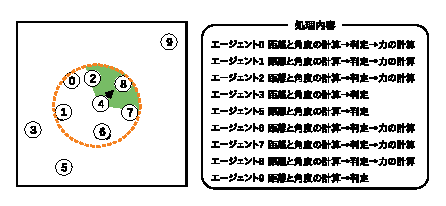
\includegraphics[width=11.5cm,clip]{figure/eikyo_hankei_siya.eps}
  \caption{視野を用いたSFMの影響範囲}
  \label{fig:siya_hani}
 \end{center}
\end{figure}

\section{本章のまとめ}

%論文引用{{{
\if 0
SFMは,人間の社会心理学的な要素と物理的な力を結びつけた物力学モデルであり,
周囲のエージェントや壁や机などの障害物から受ける力を用いてエージェントの
進行方向や速度を決定する.
人間の社会心理学的な要素は,周囲に人がいるときに避けようとする人間の心理を
利用したものである.物理学的な力は,人と人や人と障害物が衝突したときに生じる
力である.
本手法は,心理的変数が組み込まれているため,災害時の避難シミュレーションによく
用いられる(参考文献[卒論を参照])
SFMの解析空間は,二次元の連続空間モデルが用いられる.



SocialFroceModel(SFM)は,周囲の状況に基づいて生成した運動方程式を用いて時間ステップ$t$ごとに
エージェントの移動を決定する.
\eq{sfm_siki1}にエージェント$i$の運動方程式を示す.
%
\begin{eqnarray}
  m_i \frac{dv_i}{dt} = m_i \frac{v_i^0 e_i - v_i}{\tau_i}
  +\sum_{j(\neq i)}f_{ij}+\sum_{W}f_{iW}
  \label{eq:sfm_siki1}
\end{eqnarray}
%
\eq{sfm_siki1}中の
右辺第一項はエージェントが目的地へ進む力を表しており,
エージェント$i$の体重$m_i$,
希望速度$v_i^0$,
目的地までの単位ベクトル$e_i$,現在の速度ベクトル$v_i$,
時定数$\tau_i$に基づいて算出される.
右辺第二項は周囲のエージェントを避ける力であり,
$f_{ij}$はエージェント$i$とエージェント$j$の相互作用力である.
また,第三項は壁などの障害物を避ける力であり,
$f_{iW}$はエージェント$i$が壁などの障害物$W$から受ける力である.
$f_{ij}$や$f_{iW}$は,\eq{sfm_siki2}と\eq{sfm_siki3}から算出する.
%
\begin{eqnarray}
  f_{ij} =  \{A_i exp [\frac{r_{ij} - d_{ij}}{B_i}  ]
  + kg(r_{ij} - d_{ij})\} n_{ij} \\ \nonumber
  + \kappa g (r_{ij} - d_{ij}) \Delta
  v^t_{ij} t_{ij}
  \label{eq:sfm_siki2}
\end{eqnarray}
%
\begin{eqnarray}
  f_{iW} = \{A_i exp[\frac{r_{i} - d_{iW}}{B_i}]
  + kg(r_{i} - d_{iW})\} n_{iW} \\ \nonumber
  + \kappa g (r_{i} - d_{iW}) (v_i t_{iW}) t_{iW}
  \label{eq:sfm_siki3}
\end{eqnarray}
%
式中の$r_i$はエージェント$i$の体の半径,
$t_{iW}$はエージェント$i$と壁$W$の垂直ベクトル,
$n_{iW}$はエージェント$i$と壁$W$の衝突面の法線ベクトル,
$A_i$はエージェント$i$のインタラクション作用,
$B_i$はエージェント$i$の反発作用,
$k$は衝突時の反発力係数,
$\kappa$は衝突時の摩擦力係数
である.
$d_{ij}, t_{ij}, n_{ij}, r_{ij}, \Delta v_{ij}$は,
エージェント$i$,$j$間の距離,
衝突面の垂直ベクトル,衝突面の法線ベクトル,体の半径の和,接線速度の差である.
また,衝突時関数$g(x)$は,\eq{gx_siki}に示すように$x$に応じてエージェント同士
の衝突を判定する.
%
\begin{equation}
  \label{eq:gx_siki}
  g(x) =
  \begin{cases}
    1 & (x<0)     \\
    0 & otherwise
  \end{cases}
\end{equation}
%
衝突時関数$g(x)$中の$x$は,エージェント同士の距離やエージェントと壁の距離であり,
衝突時であれば1,衝突していなければ0となる.
\fi
%}}}



%1ブロックが10×30文字です
%
%\chapter{背景(1671文字)}

%***** END ************************************************

% vim: set tabstop=4 foldmethod=marker foldlevel=0 :
%**********************************************************
%\chapter{一般的にはサーベイ内容とかを書く}
\chapter{一般的なSFMの高速技法}
\label{sec:survey}
%**********************************************************
SFMを用いた人流シミュレーションは,解析人数が多くなるほど計算負荷が
膨大になるため,解析に時間がかかる.
SFMの解析時間を削減するために,モデルの単純化(参考文献)や
エージェント間距離の計算回数削減手法(参考文献),
単位時間あたりの計算回数の増加手法 (参考文献),
経路選択時の判定回数の削減手法(参考文献)などが提案されている.
本章では,SFMの各高速化手法について述べる.

\section{モデルの簡易化}
SFMの簡易化手法は,SFMの計算負荷を削減するために,
エージェント同士や壁や机などの障害物から受ける力,
進行方向を単純化する手法である.
SFMの簡易化手法の一つに一次元歩行者モデルがある(参考文献).
一次元歩行者モデルは,エージェントの動きをxやyのみにする手法である.
図\ref{fig:ichijigen_ex}に避難シミュレーション時のSFMと一次元歩行者モデルの例を示す.
図\ref{fig:ichijigen_ex}中の(a)はSFMなどの二次元連続空間モデルを示し,
(b)は一次元連続歩行者モデルの例を示す.
一次元歩行者モデルは,図\ref{fig:ichijigen_ex}のように,エージェントの動きを
算出する式を一次元に変更することで,計算負荷を削減できる.
本手法は,人の流れ(流量)を解析する場合では,
高速かつ許容できる誤差の範囲で解析できることが報告されている(参考文献).
一方で,一次元でエージェントの動きを再現するため,人の押し合いや
図\ref{fig:atigenshou}のようなアーチ現象などを再現できない.
このため,人の押し合いやアーチ現象を再現したい場合には,
一次元歩行者モデルなどのモデルを簡易化しない高速化技法を用いることが
望ましい.


\begin{figure}[hbtp]
 \begin{center}
  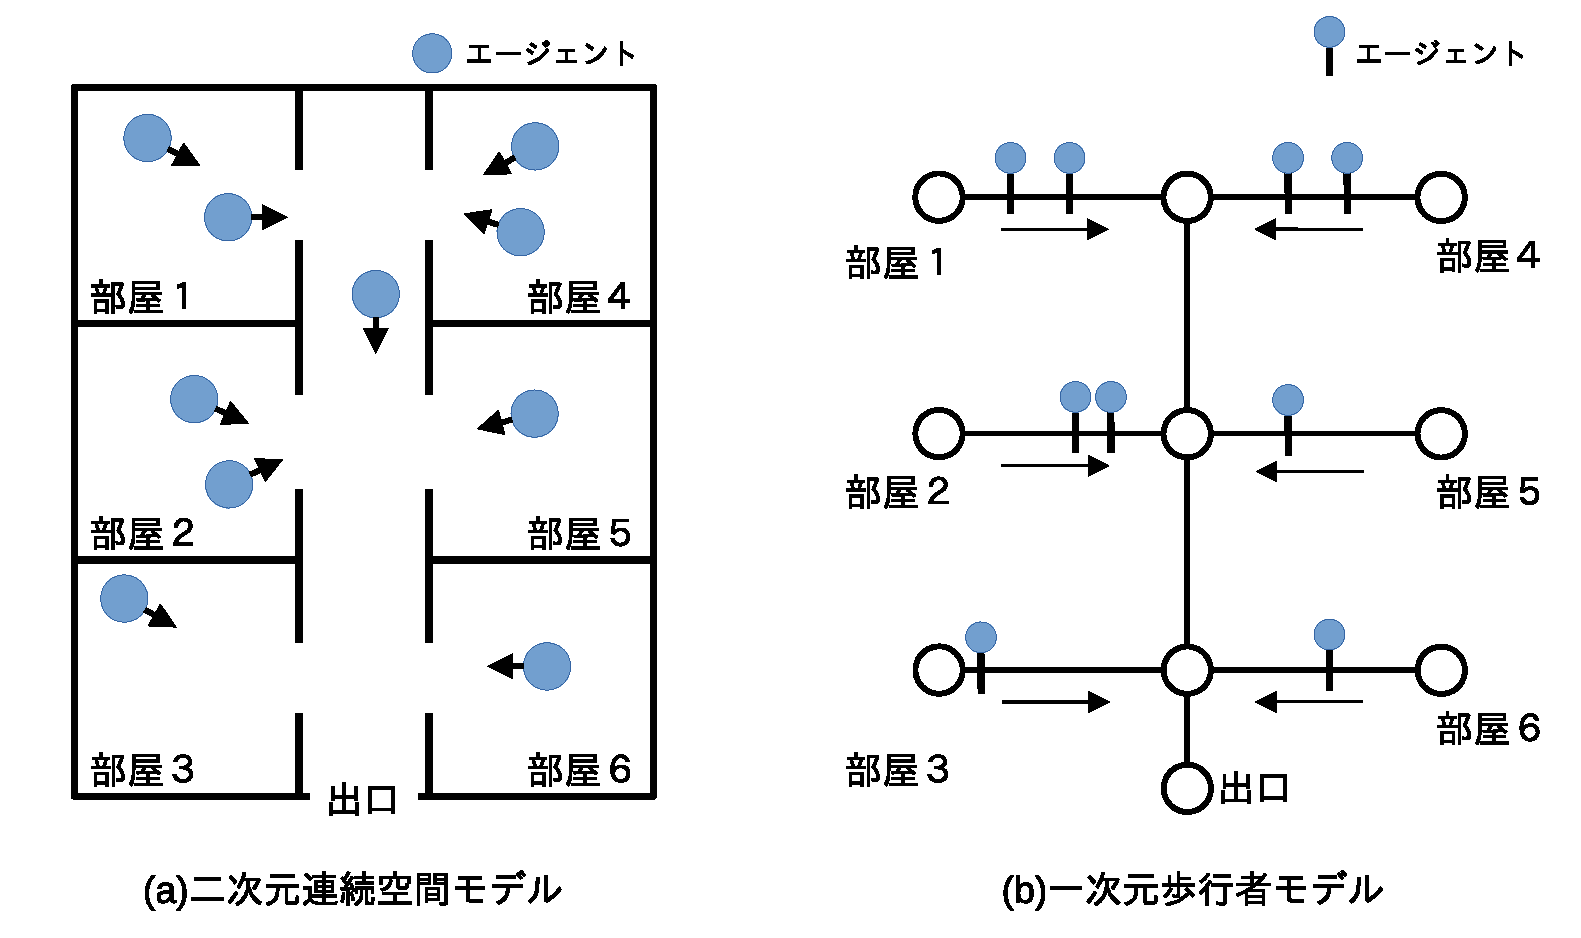
\includegraphics[width=11cm,clip]{figure/ichijigen_ex.eps}
  \caption{一次元モデルの例}
  \label{fig:ichijigen_ex}
 \end{center}
\end{figure}

\begin{figure}[hbtp]
 \begin{center}
  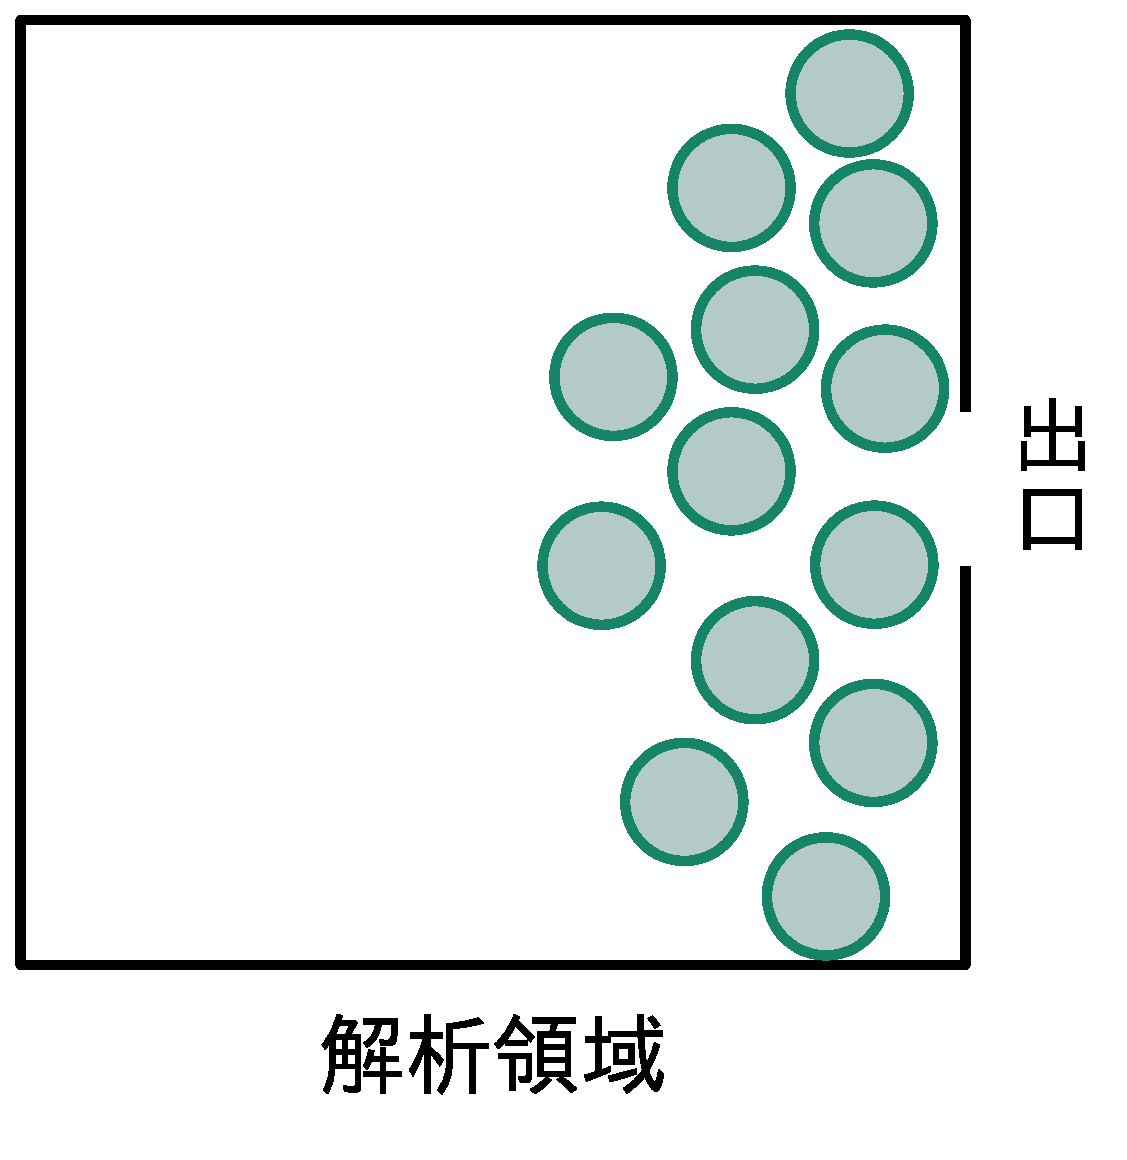
\includegraphics[width=4.5cm,clip]{figure/atigenshou.eps}
  \caption{アーチ現象の例}
  \label{fig:atigenshou}
 \end{center}
\end{figure}

\section{エージェント間の距離の計算回数削減}
SFMは,解析人数が増加するほど周囲のエージェントから受ける力の計算に
必要な周囲のエージェントが影響範囲内外かの判定の回数が増加する.
周囲のエージェントが影響範囲内外かの判定は,ルートなどを用いて
エージェント間距離$d_{ij}$を求める必要があるため,
特にエージェント間距離$d_{ij}$の計算に時間がかかる.
このため,SFMを用いた人流シミュレーションの解析時間を削減するためには,
エージェント間距離$d_{ij}$の計算回数を削減することが有効である.
エージェント間距離の計算回数削減手法にセル分割法や視野パラメータを用いた
削減手法がある.

\subsection{セル分割法}
セル分割法は,水や空気などの動きを解析できるMPS法\cite{mps}や銀河系などの圧縮性
流体に用いられるSPH法\cite{sph}などの粒子法によく用いられている.
粒子法は,近傍の粒子と相互作用する
力を計算し,粒子の行動を決定する.このため,セル分割法は,粒子法と同じように近傍の
エージェントとの相互作用力を計算するSFMに対しても用いられる.
本手法は,解析領域を格子上のセルに分割し,計算するエージェントの存在する
セルと近傍のセルに存在するエージェントに対して他のエージェントから受ける力の範囲であるか
判定し,範囲内であれば他のエージェントから受ける力を計算する手法である.
図\ref{fig:seru_ex1}にセル分割法を用いるSFMの例を示
す.図\ref{fig:seru_ex1}中の赤丸は他のエージェントから受ける力の計算をするエージ
ェント,黒丸は他のエージェント,四角は解析領域を格子状に分割したセルである.
この例では,エージェント4の行動を更新する際に青色のセル内に存在するエージェント
のみを参照するため,エージェント番号3,5,9の計算を削減できる.このとき,
視野を用いるSFMは,速度計算するエージェントの進行方向前方に存在するエージェント情報を
用いて計算するため,エージェントの進行方向後方のセルに存在するエージェント情報は不要になる,
このため,視野を用いるSFMでは,視野を考慮し,参照するセルを視野範囲に近づけることで,
計算回数を減らすことができる.

\begin{figure}[hbtp]
 \begin{center}
  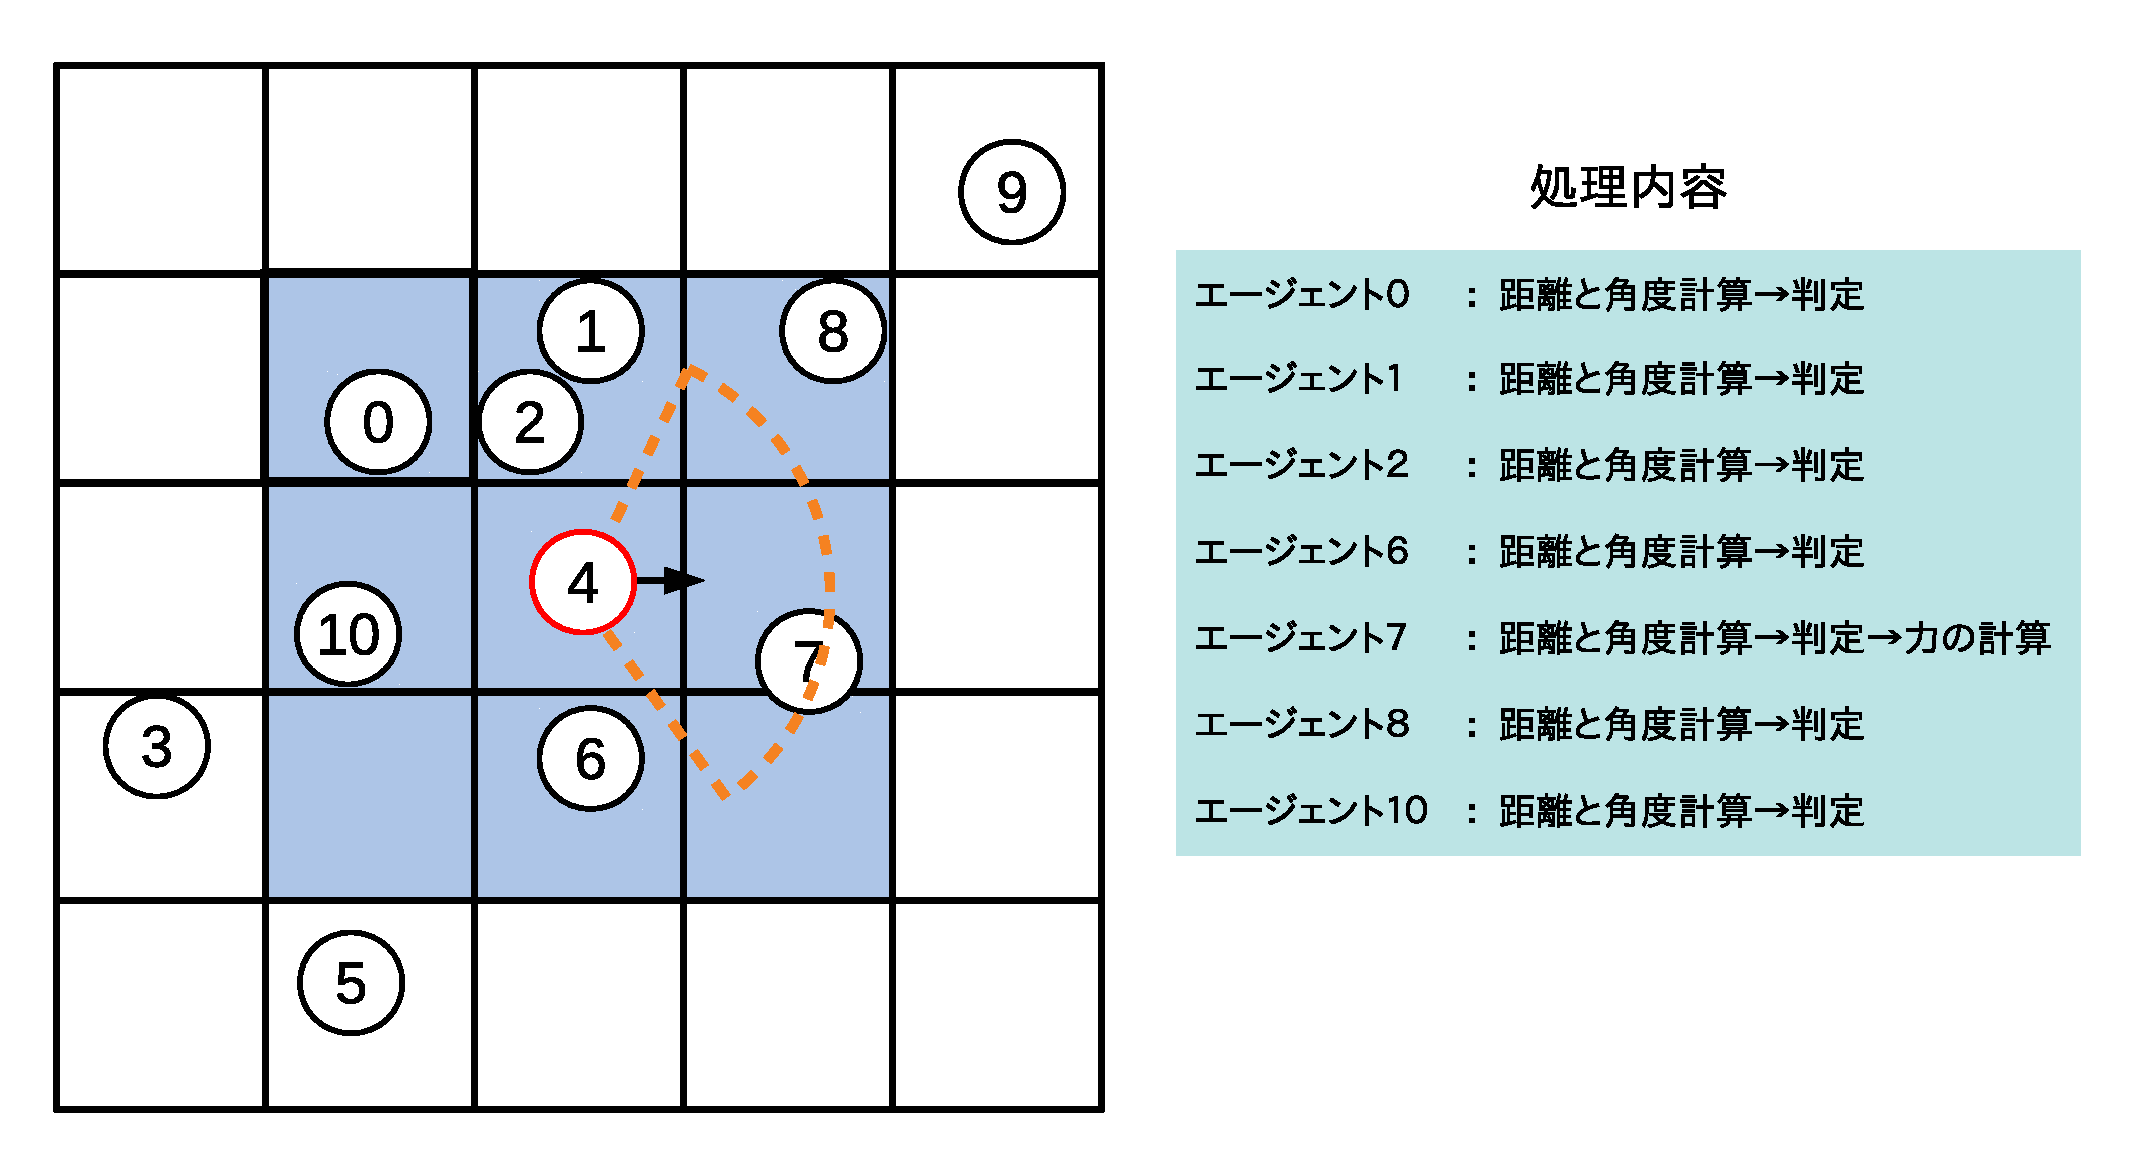
\includegraphics[width=11.5cm,clip]{figure/seru_ex1_r2.eps}
  \caption{セル分割法を用いた例}
  \label{fig:seru_ex1}
 \end{center}
\end{figure}


\subsection{視野パラメータを用いた削減手法}
視野パラメータを用いたSFMでは,


\section{単位時間あたりの計算回数}

\subsection{エージェントごとの並列性を用いた手法}

\begin{figure}[hp]
 \begin{center}
  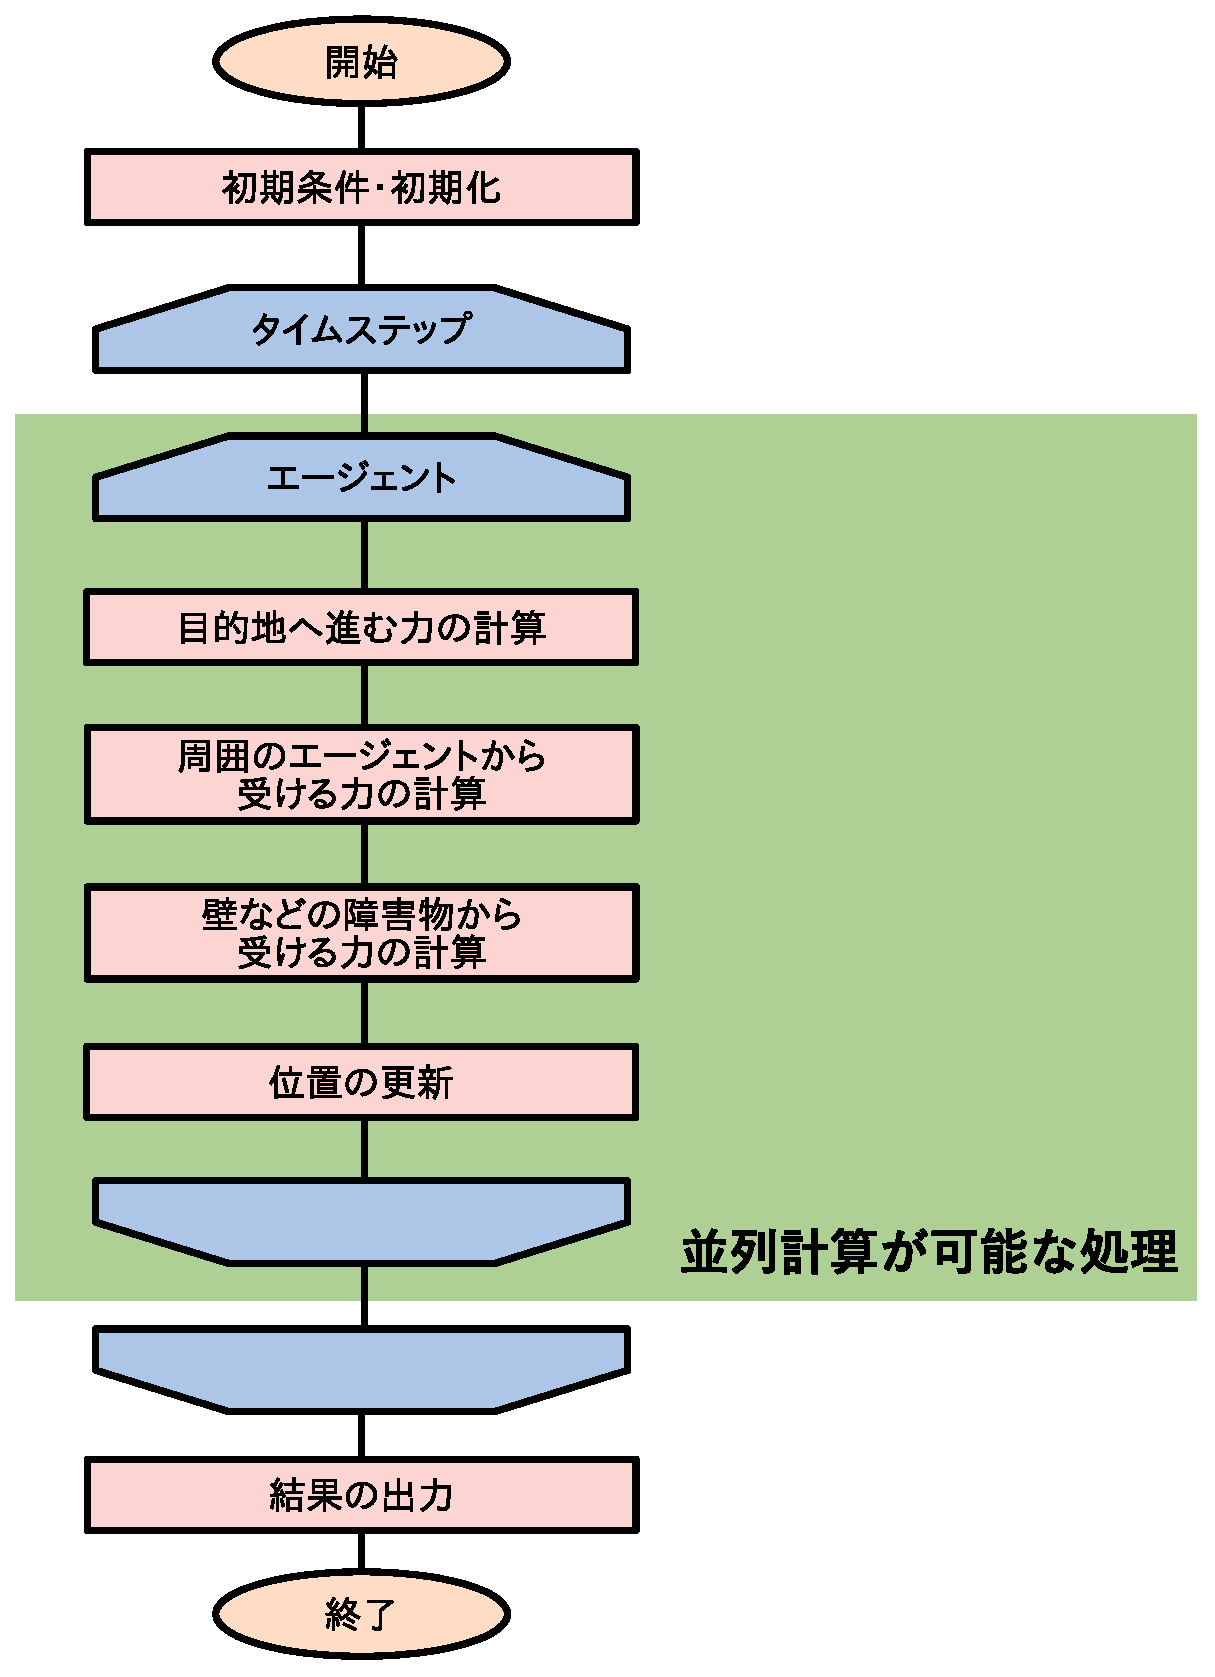
\includegraphics[width=10cm,clip]{figure/heiretuka_sfm.eps}
  \caption{SFMの並列化可能な処理}
  \label{fig:atigenshou}
 \end{center}
\end{figure}

\begin{figure}[hp]
 \begin{center}
  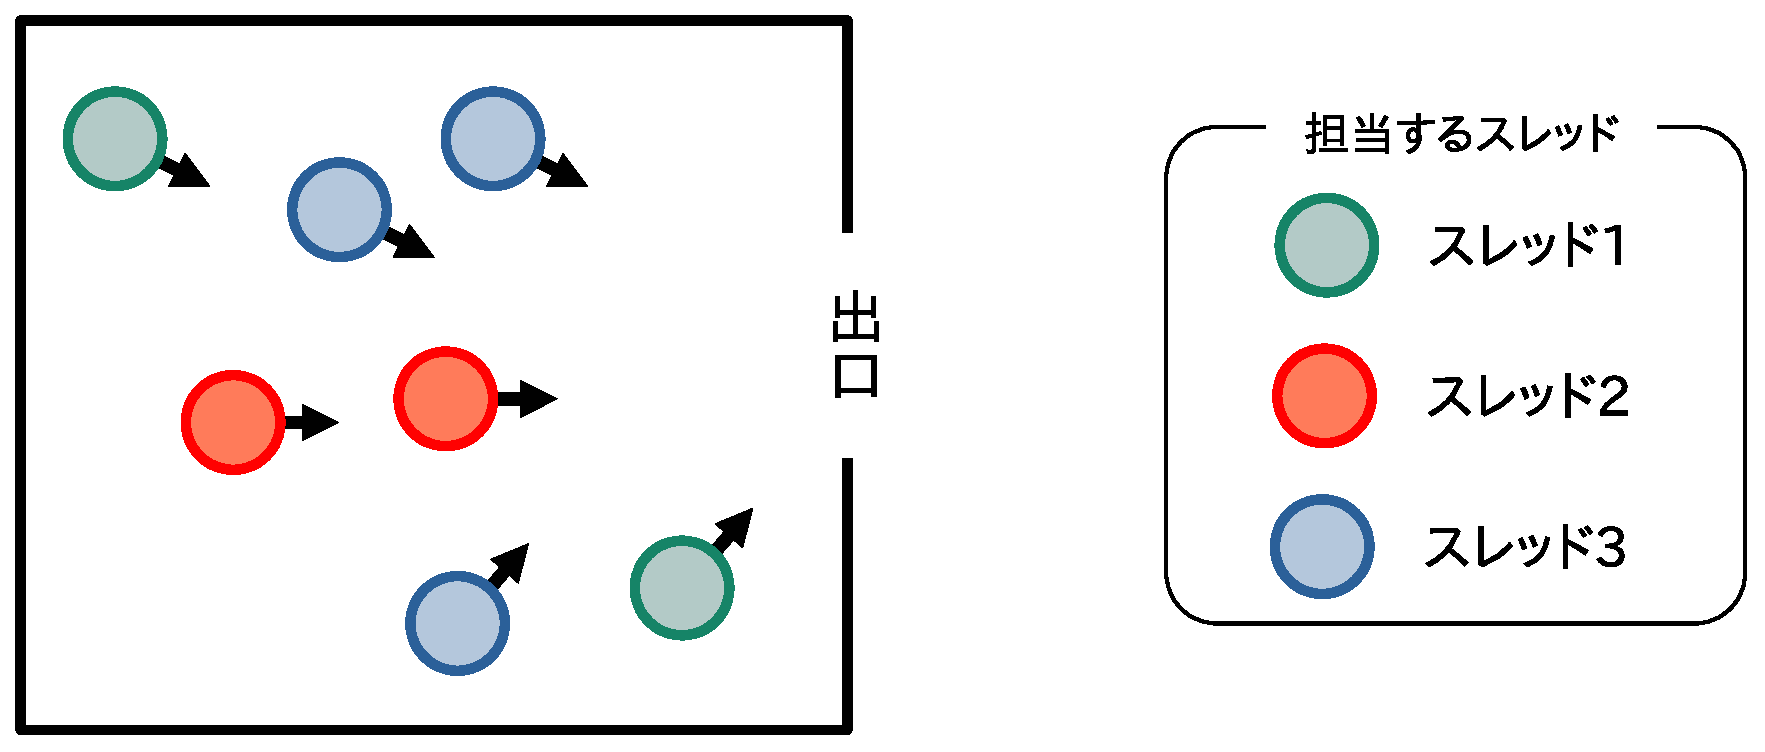
\includegraphics[width=10cm,clip]{figure/sureddo_heiretu.eps}
  \caption{3スレッドでの並列化の例}
  \label{fig:atigenshou}
 \end{center}
\end{figure}


\begin{figure}[hbtp]
 \begin{center}
  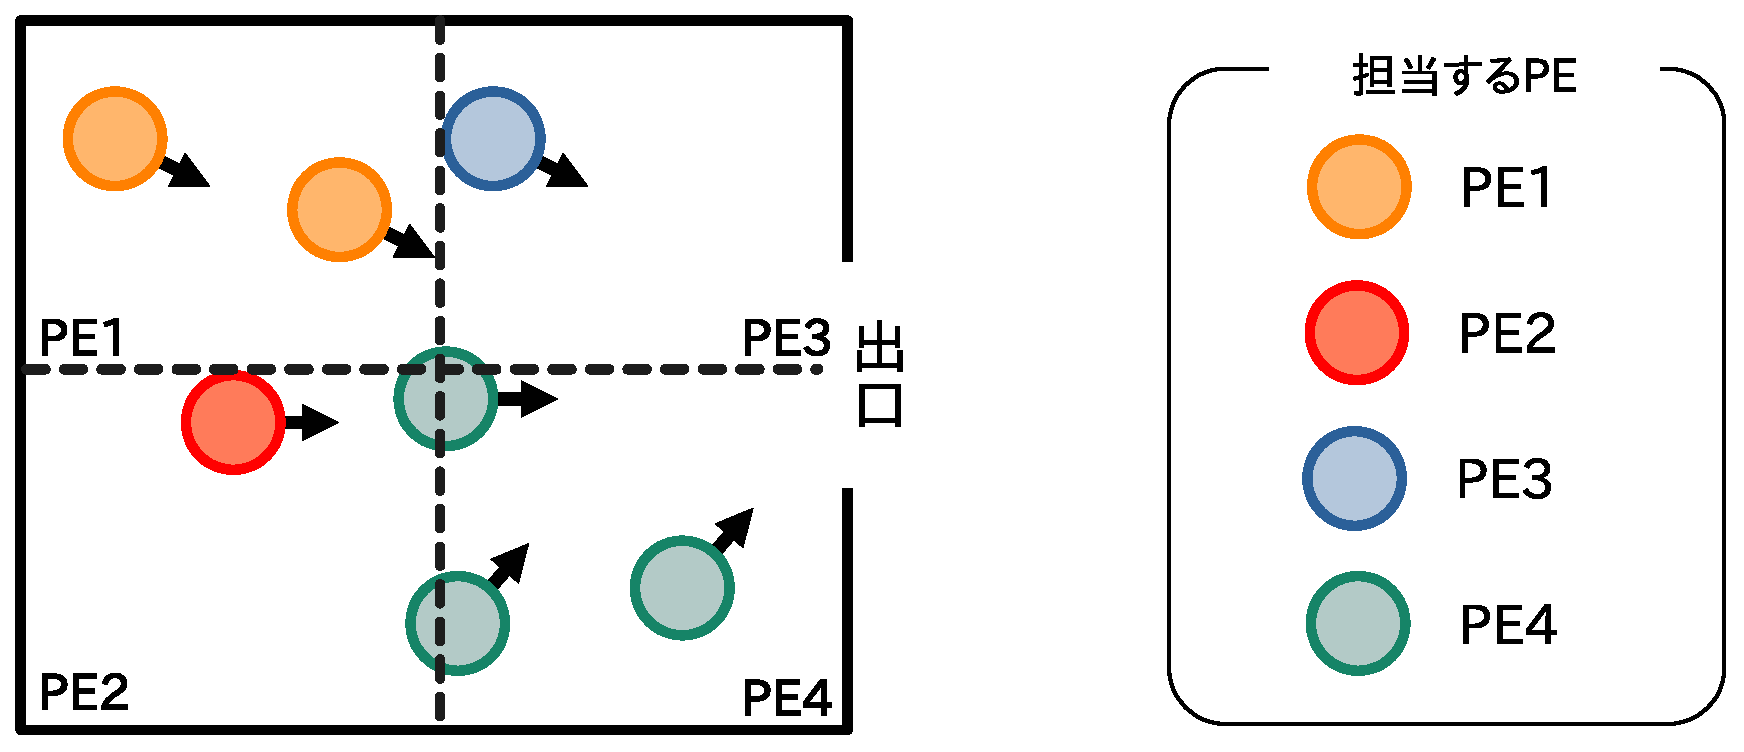
\includegraphics[width=10cm,clip]{figure/ryoiki_heiretu.eps}
  \caption{領域分割の例}
  \label{fig:atigenshou}
 \end{center}
\end{figure}


\clearpage

\subsection{解析領域ごとの並列性を用いた手法}
aaAa

\section{経路選択時の判定回数削減}
aa

\subsection{経路選択の単純化}
aa

\subsection{経路選択手法の~~}
aa

%***** END ************************************************

% vim: set tabstop=4 :
%**********************************************************
%\chapter{提案手法にあたる章}
%\chapter{格子分割を用いた進行方向計算の削減手法}
\chapter{エージェント間距離の計算回数削減}
\label{sec:reduce_distance}
%**********************************************************
SFMの運動方程式では,エージェント間距離が大きいほどエージェント間に働く相互作用力が小さくなる.
このため,SFMでは,影響半径$R_{c}$を用いてエージェント間距離の計算回数を削減するのが一般的である.
\figref{fig:sougo_hani}にエージェント4の影響半径の例を示す.また\figref{fig:serubunkatu_siya}に
\figref{fig:sougo_hani}にセル分割法を用いた例を示す.
%
\figtb{影響範囲の例}{An example of the scope of influence.}{5}{20230614_hanni_ex.eps}{sougo_hani}
%
\figtb{視野を用いたSFMにセル分割法を適用した例}{}{5}{serubunkatu_siya.eps}{serubunkatu_siya}
%
\figref{fig:sougo_hani}および\figref{fig:serubunkatu_siya}中の〇はエージェントであり,
オレンジ色の点線で囲まれた領域がエージェント4の影響範囲である.
また\figref{fig:serubunkatu_siya}中の四角はセル分割法の格子,青色の四角はセル分割法における
周辺のエージェントが影響範囲内かの判定に用いるセルである.
影響半径$R_{c}$は影響範囲の半径であり,
影響範囲外から受ける力を0とすることで,
運動方程式を計算する際に演算を省略することができる.
一方,視野を用いたSFMでは,視野範囲外の相互作用力を0とする.
\figref{fig:sougo_hani}の例で,エージェント4が図中矢印の方向に移動する際には,
エージェント4の視野は,図中の緑色の領域のように設定され,
視野$\subseteq$影響範囲のような関係となる.

SFMで用いられるエージェント間距離の計算回数削減手法は,
影響範囲が円形であることを前提としており,
影響範囲が視野のように扇形の場合を想定していない.
例えば,\figref{fig:sougo_hani}のエージェント配置では,
半径$R_{c}$内の白い領域に存在する5つのエージェントが視野外にあるにも関わらず,
これらのエージェントに対するエージェント間距離の計算が必要となる.
人の視野角$\theta$は$\pi$以下であるため,
視野を用いたSFMに一般的なSFMのエージェント間距離の計算回数削減手法を用いると,
影響範囲を円形に絞り込みをした上で,%視野形状に合わせた
扇形に絞り込みを行う操作が必要となる.
このため,視野範囲外となる半径$R_{c}$内のエージェントが多く存在するほど,
相互作用力を0として計算するエージェントに対するエージェント間距離の計算回数が増える.
このため,本章では,
視野形状である扇形に近似した領域を設定し,
近似領域外のエージェントに対するエージェント間距離の計算回数を削減することで,
視野を用いたSFMを高速化する手法について述べる.
%fig{serubunkatu_siya}を使ってセル分割法の話を入れたい

\section{近似領域の選択方法}
提案手法では,近似領域の算出に必要な計算時間を最小限に抑えるために,
長方形で視野範囲を近似する.
これに合わせて,
視野範囲はエージェントの進行方向前方に存在するため,
エージェントの進行方向を長方形の辺数に合わせて上下左右の4パターンに分類し,
エージェントの進行方向に応じた近似領域を設定する.
\figref{fig:sentaku}に上下左右の4パターンの近似領域を示す.
\figref{fig:sentaku}中の◯はエージェント,矢印は進行方向,格子はセル分割法のセル,
青い四角は,各進行方向ごとの近似領域である.
\figref{fig:sentaku}の近似領域の選択方法は,エージェントの座標や進行方向などといった
複数の選択方法が考えられる.
エージェントの進行方向の分類方法によりシミュレーション時間が変化する可能性があるため,
本論文では,既存手法であるセル分割法を含む6パターン実装し,その有効性を評価する.
提案手法であるパターン2~6は,いずれの手法もパターン1のセル分割法の考え方を基にしており,
時間ステップごとに影響範囲の近似領域を設定した上で,
近似領域内で影響範囲内となるエージェントを相互作用力を計算する対象として設定する.

%\figtb{エージェント4の実装パターンごとの近似領域の例}{The approximation region for each pattern of agent 4.}{9}{20231007_hanni.eps}{90do_hamideru}

\figtb{進行方向ごとの近似領域}{}{8}{20220225_sentaku.eps}{sentaku}

\subsection{パターン1(セル分割法)}
パターン1は,一般的なセル分割法\cite{cell1}\cite{cell2}によるエージェント間距離の計算回数を削減する.
\figref{fig:patan1_ex}に\figref{fig:sougo_hani}中のエージェント4にパターン1を用いて
近似領域を設定した例を示す.
セル分割法は,\figref{fig:patan1_ex}のように解析領域を格子状に分割し,
影響半径$R_{c}$の円内に重なるセルを近似領域とする手法である.
本手法は,分割するセルのサイズを影響半径と同じ距離に設定することで,
近似領域をエージェントの近傍9セルに限定することができる.
本例では,エージェント4の近傍9セルは黄色のセルであり,
それ以外のセルに属するエージェント3,5,9に対するエージェント間距離の計算を削減できる.
なお,セル分割法は相互作用力を計算する範囲を円形で想定した手法であるため,
近似領域が正方形となることから,パターン1の実装では進行方向の推測は行わない.
また,本論文では,セル分割法のなかでもメモリ使用量を抑えることができると知られている
連結リスト法\cite{cell_book1}\cite{cell_renketu}を用いる.

\figtb{パターン1を用いたエージェント4の近似領域}{}{4}{patan1_ex}{patan1_ex}

\begin{table}[t]
	\centering
	\caption{パターン2,3の進行方向判定条件}
	\label{tb:patan2_joken}
	\begin{tabular}{c|cccc}
		\hline \hline
		& 右 & 左 & 上 & 下  \\ \hline
		条件1
		& $\frac{1}{\sqrt{2}} < e_x \leq 1$
		& $ -1 \leq e_x < \frac{-1}{\sqrt{2}}$
		& $ \frac{-1}{\sqrt{2}} < e_x < \frac{1}{\sqrt{2}}$
		& $ \frac{-1}{2} < e_x < \frac{1}{2} $ \\ \hline
		条件2 
		& $\frac{-1}{2} < e_y < \frac{1}{2} $ 
		& $\frac{-1}{2} < e_y < \frac{1}{2} $
  	& $ \frac{1}{\sqrt{2}} < e_y \leq 1$
		& $ -1 \leq e_y < \frac{-1}{\sqrt{2}} $ \\ \hline
	\end{tabular}
\end{table}

\subsection{パターン2(進行方向を用いた近似)}
パターン2は,エージェントの進行方向を表す単位ベクトル$e_{i}$を参照することで,
パターン1の近似領域を視野範囲に近づける手法である\cite{katayose}.
\tabref{tb:patan2_joken}にパターン2の近似領域を選択するための条件を示す.
\tabref{tb:patan2_joken}中の条件1と条件2の両方を満たす進行方向から近似領域を選択する.
本手法は,\tabref{tb:patan2_joken}の条件に基づいて
単位ベクトル$e_{i}$が示す進行方向を上下左右を$\frac{1}{2}\pi$の均等な角度で分割し,
セル分割法の近似領域から\figref{fig:sentaku}のように進行方向の反対側にある3セルを除外する.
\figref{fig:patan2_ex}に\figref{fig:sougo_hani}の例におけるエージェント4の近似領域を
パターン2を用いて選択した例を示す.
\figref{fig:patan2_ex}の例では,エージェントの進行方向は右と判定され,
\figref{fig:sentaku}に示す右方向の青いセルを近似領域に設定する.
このため,白色のセルに存在するエージェントに対する距離計算を削減できる.
パターン2は,進行方向を必ず上下左右のいずれかに設定するため,
常に近似領域が6セルとなり,セル分割法の9セルに比べて近似領域の面積を$\frac{2}{3}$に削減できる.
一方で,\figref{fig:patan2_ex}のように視野範囲全体が近似領域内に含まれる保障がないため,
本来相互作用力の計算が必要なエージェントに対する計算を削減し,誤差が発生する可能性がある.

\figtb{パターン2を用いたエージェント4の近似領域}{}{5}{patan2_ex}{patan2_ex}

\subsection{パターン3(視野座標と進行方向を用いた近似)}
パターン3は,パターン2で発生する誤差を防ぐために,
近似領域外に視野範囲が存在しないかを判定する処理を追加し,
セル分割法と同じ精度を保つ手法である\cite{katayose}.
本手法は,\tabref{tb:patan2_joken}を用いてパターン2の近似領域を導出したのち,
視野の座標$(L_x,L_y)$,$(R_x,R_y)$が
近似領域内のセルであればパターン2の近似領域を用いて相互作用力を計算し,
そうでなければパターン1の近似領域を用いて相互作用力を計算する.
\figref{fig:patan3_good}にパターン3を用いて近似領域を削減できる例を示す.
\figref{fig:patan3_good}中の緑色の視野領域上に存在する黒点は,視野の座標
である$(L_x,L_y)$と$(R_x,R_y)$を示す.
\figref{fig:patan3_good}の例では,\tabref{tb:patan2_joken}中の進行方向が右
の条件を満たし,視野の座標$(L_x,L_y)$と$(R_x,R_y)$が青色の近似領域内であるため,
\figref{fig:sentaku}に示す右方向の青いセルが近似領域になり,セル分割法よりも
近似領域を削減できる.
一方で,\figref{fig:sougo_hani}中のエージェント4にパターン3の条件を適用した場合は,
\figref{fig:patan3_ex}のように,視野の座標$(L_x,L_y)$が\figref{fig:sentaku}の
青いセル以外に存在するため,近似領域がパターン1と同様に近傍9セルとなる.
エージェントの座標は時間ステップごとに変化するため,
パターン3を用いると,進行方向が変化しないエージェントに対しても
すべての時間ステップでパターン1よりもエージェント間距離の計算を削減できるとは限らない.
一方で,パターン3は,パターン1のセル分割法と同じ精度のシミュレーション結果を得ることができる.

\figtb{パターン3を用いた近似領域の削減例}{}{4.75}{patan3_good}{patan3_good}

\figtb{パターン3を用いたエージェント4の近似領域}{}{4.75}{patan3_ex}{patan3_ex}

\subsection{パターン4(視野座標を用いた近似)}
パターン4は,視野の左右両端の座標$(L_x,L_y)$,$(R_x,R_y)$を用いて近似領域を設定する手法である.
視野範囲は進行方向の前方に存在するため,
視野の左右両端の座標はエージェント座標から見て必ず進行方向側となる.
この特性を利用し,パターン4では,\tabref{tb:patan4_joken}に示すように,
エージェント座標$(A_x,A_y)$と視野座標$(R_x,R_y)$,$(L_x,L_y)$の
大小関係を用いて進行方向を判定する.
本手法の\tabref{tb:patan4_joken}に満たない場合は,パターン1と同様に近傍9セルを近似領域にする.
\figref{fig:patan4_good}にパターン4を用いた近傍領域の削減例を示す.
\figref{fig:patan4_good}の例では,エージェント座標$(A_x,A_y)$と
視野座標$(R_x,R_y)$,$(L_x,L_y)$が\tabref{tb:patan4_joken}中の
条件である$R_x \geq A_x$および$L_x \geq A_x$が成り立つため,進行方向が右と判定され,
\figref{fig:sentaku}の右方向の青いセルが近似領域となる.
\figref{fig:patan4_ex}に\figref{fig:sougo_hani}中のエージェント4にパターン4を用いて
近似領域を決定した例を示す.
\figref{fig:patan4_ex}の例は,\tabref{tb:patan4_joken}中の判定条件を満たす進行方向がないため,
パターン1と同様に近傍9セルを近傍領域とする.

\begin{table}[t]
	\centering
	\caption{パターン4の進行方向判定条件}
	\label{tb:patan4_joken}
	\begin{tabular}{c|c|c|c|c}
		\hline \hline
		& 右 & 左 & 上 & 下  \\ \hline
		条件1 & $R_x \geq A_x$ & $R_x < A_x$ & $R_y \geq A_y$ & $R_y < A_y $ \\ \hline
	  条件2 & $L_x \geq A_x$ & $L_x < A_x$ & $L_y \geq A_y$ & $L_y < A_y$ \\ \hline
	\end{tabular}
\end{table}

\figtb{パターン4を用いた近似領域の削減例}{}{5}{patan4_good}{patan4_good}

\figtb{パターン4を用いたエージェント4の近似領域}{}{5}{patan4_ex}{patan4_ex}


\subsection{パターン5(視野座標とセルの座標を用いた近似)}
パターン(視野座標とセルの座標を用いた近似方法)5は,セル分割法のセル座標と視野範囲の左右両端の座標$(L_x,L_y)$,$(R_x,R_y)$を
用いて近似領域を設定する手法である.
本手法は,運動方程式を算出するエージェントが所属するセルの
左上座標$(x_1,y_2)$および右下座標$(x_2, y_1)$を用いて,
\figref{fig:sentaku}の4パターンの水色の領域内に視野が収まっているかを判定する.
\tabref{tb:patan5_joken}にセルの
左上座標$(x_1,y_2)$および右下座標$(x_2, y_1)$を用いたパターン5の判定条件を示す.
また,\figref{fig:patan5_good}にパターン5を用いた場合の近似領域を削減する例を示す.
\figref{fig:patan5_good}の例では,\tabref{tb:patan5_joken}中の
$R_x \geq x_1$および$L_x \geq x_1$が成り立つため,進行方向は右と分類される.
このため,\figref{fig:patan5_good}の例では,近似領域は図中の青いセルとなる.
\figref{fig:patan5_ex}に\figref{fig:sougo_hani}中のエージェント4にパターン5を用いて
近似領域を選択した例を示す.
\figref{fig:patan5_ex}の例では,
$R_y \geq y_1$および$L_y \geq y_2$が成り立つため,進行方向は上と分類される.
本手法は,エージェントのセル上の位置に応じて進行方向を分類するため,
ベクトル$e_i$の表す進行方向が同じエージェントでも
エージェント座標に応じて異なる方向に分類される可能性がある.
本手法も\tabref{tb:patan5_joken}のいずれの条件にも当てはまらない場合は,
パターン1(セル分割法)と同様に近傍9セルを近似領域とする.

\begin{table}[t]
	\centering
	\caption{パターン5の進行方向判定条件}
	\label{tb:patan5_joken}
	\begin{tabular}{c|c|c|c|c}
		\hline \hline
		& 右 & 左 & 上 & 下  \\ \hline
 		条件1 & $R_x \geq x_1$ & $R_x < x_2$ & $R_y \geq y_1$ & $R_y < y_2 $ \\ \hline
		条件2 & $L_x \geq x_1$ & $L_x < x_2$ & $L_y \geq y_1$ & $L_y < y_2 $ \\ \hline
	\end{tabular}
\end{table}

\figtb{パターン5を用いた近似領域の削減例}{}{5}{patan5_good}{patan5_good}

\figtb{パターン5を用いたエージェント4の近似領域}{}{5}{patan5_ex}{patan5_ex}

\clearpage
\subsection{パターン6(誤差が生じないように進行方向を用いた近似)}
パターン6は,パターン2で設定した上下左右の角度範囲を,
シミュレーション誤差の出ない範囲で設定する手法である.
パターン6では,
\figref{fig:sentaku}中の水色の領域である近似領域内に視野範囲がすべて収まる進行方向を静的に計算し,
エージェントの進行方向を表すベクトル$e_i$の閾値を定める.
視野角を$\theta_{view}$とおくと,
エージェント座標がどの位置であっても上方向と判定される進行方向の角度は
$\frac{1}{2}(\pi - \theta_{view})$から$\frac{1}{2}(\pi + \theta_{view})$の間であり,
これを用いて進行方向ベクトル$e_{i} = (e_{x}, e_{y})$の範囲が
$\sin{(\frac{1}{2}(\pi - \theta_{view}))} \leq e_{x}$という条件を設定できる.
\tabref{tb:patan6_joken}にパターン6の進行方向判定条件を示す.
パターン6は,パターン3~6のように視野座標$(R_x,R_y)$および$(L_x,L_y)$を算出する必要がないため,
他の分類条件よりも高速に進行方向を分類することができる.
一方で,進行方向が特定の方向である場合は,
エージェント座標に関係なくパターン1(セル分割法)と同じ近似領域を設定するため,
エージェント間距離の計算回数は,パターン1に次いで多くなると考えられる.

\begin{table}[t]
	\centering
	\caption{パターン6の進行方向判定条件}
	\label{tb:patan6_joken}
	\begin{tabular}{c|c|c|c}
		\hline \hline
		右 & 左 & 上 & 下  \\ \hline
		$ \cos(\frac{1}{2}\theta_{view}) \leq  e_y $ 
		& $ e_y \leq -\cos(\frac{1}{2}\theta_{view})$ 
		& $ \sin(\frac{1}{2}(\pi - \theta_{view})) \leq e_x $ 
		& $ e_x \leq \sin(\frac{1}{2}(\pi - \theta_{view}))  $ \\ \hline
	\end{tabular}
\end{table}

\clearpage

%tb:定数設定
\begin{table}[tb]
  \begin{center}
    \caption{測定条件}
    \label{tb:tab_para}
    \begin{tabular}{c|c}
      \hline \hline
      $A_i$            & 2000N                              \\ \hline 
      $B_i$            & 0.08m                              \\ \hline 
      $k$              & $1.2 \times 10^5 kg s^{-2} $       \\ \hline 
      $\kappa$         & $2.4 \times 10^5 kg m^{-1} s^{-2}$ \\ \hline 
      $v_i^0$          & $1.4$m/s                           \\ \hline 
      $m_i$            & $80$kg                             \\ \hline 
      $\tau_i$         & 0.5                               \\ \hline 
      $r_i$            & $0.25$m                            \\ \hline 
		視野角         & $\frac{2}{3}\pi$                   \\ \hline 
      視野距離         & $20$m                              \\ \hline 
      タイムステップ数 & 25000                              \\ \hline
    \end{tabular}
  \end{center}
\end{table}

\figtb{エージェントの初期配置}{Initial position of agents.}{4}{20221031_haichi.eps}{agent_haichi}

\section{評価}
視野を用いたSFMに対するエージェント間距離の計算回数削減手法の有効性を確認するために,
既存手法であるセル分割法を用いたパターン1および提案手法である
パターン2~6を用いて人流シミュレーションを行う.
評価環境は,
CPUがIntel Xeon CPU E5-2687w v2, 
メモリが64GB,
OSがLinux 4.12.9であり,
プログラムのコンパイルにはgcc 7.2.0で-O3オプションを設定する.
また,本評価では,
視野を用いたSFMで期待される押し合い圧し合いを行う群衆の行動を再現するために,
エージェントの初期配置および目的地を\figref{fig:agent_haichi}のように設定し,
\tabref{tb:tab_para}を用いて運動方程式を計算する.%\Cite{sfm_para2}
\tabref{tb:tab_para}のパラメータは文献[2]を参考に設定したものであり,
これを踏まえてセル分割法のセルサイズは視野範囲に合わせて20mとする.
本測定では,\figref{fig:agent_haichi}の緑色の範囲内にエージェントをランダムに生成し,
各エージェントの目的地を解析領域上で初期配置と点対称となる座標に設定することで,
解析領域の中央でエージェントが密集した状態を作る.

%tb:評価環境
\if 0
\begin{table}[tb]
  \begin{center}
    \caption{評価環境}
    %\ecaption{The evaluation environment.}
    \label{tb:com_env}
    \begin{tabular}{c|c}
      \hline \hline
      CPU              & Intel Xeon CPU E5-2687w v2 \\ \hline
      メモリ           & 64GB                       \\ \hline
      OS               & Linux 4.12.9               \\ \hline
      コンパイラ       & gcc 7.2.0                  \\ \hline
      最適化オプション & -O3                        \\ \hline
    \end{tabular}
  \end{center}
\end{table}
\fi


%tb:計算回数
\begin{table}[tb]
\begin{center}
\caption{エージェント間距離の計算回数[$10^{10}$回]}
\label{tb:count_result_yobi}
\begin{tabular}{c|r|r|r|r|r|r}
\hline \hline
	人数 & パターン1 & パターン2 & パターン3 & パターン4 & パターン5 & パターン6 \\  
	\hline
	\multirow{2}{*}{3000} 
	& 5.1   & $\mathbf{3.9}$   & 4.0    & 4.4    & 4.1    & 4.4   \\  
	&       & ($\mathbf{24.5}$\%) 					& (22.9\%) & (15.3\%) & (20.7\%) & (15.2\%) \\ \hline
	\multirow{2}{*}{5000} 
	& 14.4  &  $\mathbf{10.9}$  					  & 11.1   & 12.2   & 11.4   & 12.2  \\  
	&       & ($\mathbf{23.8}$\%) 					& (22.6\%) & (15.2\%) & (20.5\%) & (15.1\%) \\ \hline
	\multirow{2}{*}{7500} 
	& 33.1  & $\mathbf{25.2}$	 		    	 	 & 25.8   & 28.3   & 26.7   & 28.3  \\ 
	&       & ($\mathbf{23.9}$\%) 					& (22.2\%) & (14.6\%) & (19.4\%) & (14.6\%) \\ \hline
    \end{tabular}
  \end{center}
\end{table}


\subsection{エージェント間距離の計算回数}
\label{sec:count}
%*************************************************
\tabref{tb:count_result_yobi}に,エージェント間距離の計算回数および削減率を示す.
表中の括弧内の数値は,削減率であり,
パターン$n$のエージェント間距離の計算回数$C_{n}$と
パターン1(セル分割法)のエージェント間距離の計算回数$C_{1}$より
\eq{sakugen}のように求める.
%
\begin{align}
	\mbox{削減率[\%]} = ( 1 - \frac{C_{n}}{C_{1}}) \times 100
    \label{eq:sakugen}
\end{align}

\tabref{tb:count_result_yobi}より,
パターン2~6はセル分割法よりもエージェント間距離の計算回数が少なく,
最も高い削減率が得られたのはパターン2であることが確認できる.
パターン2は近似領域が視野範囲全体を含まない可能性のある手法であるが,
セル分割法と同じ解析精度の手法に限定しても,
パターン2と同じ手順で進行方向を判定したパターン3が最も高い削減率である.
パターン3で高い削減率が得られたのは,
エージェントの初期配置を\figref{fig:agent_haichi}のように設定したことにより,
\tabref{tb:patan2_joken}で削減可能な角度の範囲の広さが削減率に強く影響したためであると考えられる.
本測定条件では,初期のエージェントの進行方向がすべて異なり,
時間経過による進行方向の変化も少ない.
実問題のシミュレーションでは,エージェントが同一の目的地を目指すものが多く,
進行方向が一定の方向に偏ることが多いため,
解析対象に応じて表1から適切なパターンを選択する必要があると考えられる.
横方向や縦方向に進むエージェントが多い問題では,パターン3の近似領域を
用いることで,より多くのエージェント間距離の計算回数が削減できる.
一方で,斜め方向に進むエージェントが多い問題では,パターン3を用いた場合に
近似領域を削減できないため,進行方向の角度に応じで使用するパターンを
決定することが有効であると考えられる.
同様に,削減率が最も低いパターン6は,
\tabref{tb:patan6_joken}の条件を満たさない角度が最も広いため,
パターン1(セル分割法)と同じ近似領域を用いることが多く,
高い削減率が得られなかったと考えられる.

また,各パターンの削減率は,エージェント数によらず一定であることが分かる.
これは,パターン2が周囲のエージェント情報を参照せずに近似領域を設定するためである.
エージェント数や,エージェントの密度が変化してもエージェントごとの近似領域の面積は変わらない.
加えて,解析領域中央付近でエージェントが密集するように条件を設定しており,
エージェント間距離の計算はほとんどが密集状態で実行されるものである.
一方,密集領域以外では,近似領域から除外した領域のエージェント数が少なくなりやすい.
これに伴い,すべての視野に対して近傍領域の面積の約3割を削減するパターン2で
\tabref{tb:count_result_yobi}の削減率が3割未満となり,
近傍領域の面積の削減率とエージェント間距離の演算回数の削減率に差が生じた.

%tb:解析時間
\begin{table*}[t]
  \caption{解析時間[s]}
  %\ecaption{Execute time.}
  \label{tb:time_result_yobi}
  \begin{center}
    \begin{tabular}{c|r|r|r|r|r|r}
      \hline \hline
          人数 & パターン1 & パターン2 & パターン3 & パターン4 & パターン5 & パターン6  \\  \hline
          3000 & 2636      & $\mathbf{2123}$      & 2140      & 2307      &  2184     & 2292      \\  \hline
          5000 & 7435      & $\mathbf{5941}$      & 6016      & 6463      &  6162     & 6453      \\  \hline
          7500 & 17198     & $\mathbf{13730}$     & 13985     & 15048     & 14931     & 15036     \\  \hline
    \end{tabular}
  \end{center}
\end{table*}

\subsection{シミュレーションの実行時間の測定}
第\ref{sec:count}節より,
提案手法であるパターン2~6を用いることで,パターン1(セル分割法)よりも
エージェント間距離の計算回数が削減できることが確認できた.
一方で,提案手法はパターン1が必要としない進行方向を求める処理を実行するため,
進行方向を求める処理の分だけ実行時間は増加する.
このため,進行方向を求めるために必要な時間を考慮しても
エージェント間距離の計算回数削減による高速化が有効であることを確認する.
\tabref{tb:time_result_yobi}にシミュレーションの実行時間を,
\figref{fig:kousokuka2}に\eq{kousokuka}より算出した高速化率を示す.
%
\begin{align}
    \centering
	\mbox{高速化率[倍]} = \frac{\mbox{パターン1の実行時間[s]}}{\mbox{パターン}n\mbox{の実行時間[s]}}
    \label{eq:kousokuka}
\end{align}
%
\tabref{tb:time_result_yobi},\figref{fig:kousokuka2}より,
提案手法であるパターン2〜6は,すべてのパターンにおいてパターン1(セル分割法)よりも1.14倍から1.25倍高速であり,
従来手法よりも解析時間が1.3割から2.0割削減できることが確認できる.
また,すべてのパターンにおいて削減率に応じた高速化率が得られており,
進行方向を求める処理を追加したことによる処理時間の時間増加は小さいといえる.
これを踏まえると,パターン2とパターン3の高速化率の差は,
本来計算が必要なエージェント間距離の計算の有無によるものであると考えられる.
つまり,パターン3はパターン2の処理に加えて視野の座標を求め,
厳密に視野範囲を予測しているが,追加の処理による実行時間の増加は小さいといえる.

\figtb{パターン1(セル分割法)に対する高速化率}{}{11}{20230226_kousokuka.eps}{kousokuka2}

\subsection{シミュレーション精度の測定}
提案手法のうち最も高速な手法はパターン2であるが,
パターン2は他の手法と異なり視野範囲の一部が近似領域外となることを許容する.
つまり,
提案手法のうちパターン2のみ,
パターン1(セル分割法)のシミュレーションと比べてシミュレーション誤差が生じる手法となる.
このため,パターン1のシミュレーション結果とパターン2のシミュレーション結果を比較し,
シミュレーション精度を確かめる.
誤差は,パターン1とパターン2が算出した時間ステップごとに各エージェントの座標を出力し,
2手法の同時刻・同エージェント同士によるエージェント間距離の最大値とした.
本測定条件下のパターン2の誤差は,エージェント数によらず約3.2cmであった.
これは,解析領域全体や人の大きさを踏まえると小さな数値であり,
シミュレーション結果として十分に実用的であると考えられる.
誤差を小さな数値で抑えることができたのは,
SFMではエージェントが目的地に向かう特性から,
時間ステップごとの位置座標に応じて進行方向が更新され,
細かな誤差が発生してもそれを蓄積しにくいためであると考えられる.
加えて,パターン2が相互作用力の計算を省略したのは視界の隅にあたる領域であり,
パターン2を用いても人の行動を自然に再現できると考えられる.

\section{本章のまとめ}%
%**********************************************************
本章では,視野を用いたSFMを高速化するために,エージェント間距離の計算回数を削減する手法を提案し,
その有効性を評価した.
評価の結果,提案手法は,エージェントが交差するように移動する問題において,
十分に許容可能な誤差の範囲で約1.25倍の高速化率が得られることを確認した.
提案手法を用いた人流シミュレーションは,従来手法よりも解析時間を最大2割削減できるため,
解析に必要な電力コストを解析時間に応じて削減できる可能性があり,
これは建物の設計に必要な開発コストの削減にもつながると考えられる.
また,本測定の提案手法で発生した誤差より大きい誤差を許容することができる場合,
近似領域の視野範囲に対する近似制度を高めることが可能であり,
エージェント間距離の計算回数の削減量を増やすことができると期待できる.
このため,精度低下を許容できる問題に対しては,さらなる高速化が見込めるといえる.

\if 0
さらに,提案手法を用いた人流シミュレーションは,
エージェントごとに独立して計算できる並列性があるため,
CPUやGPUを用いて並列処理することで
高速に解析できると考えられる.
特にGPUを用いた人流シミュレーションは,GPU上でエージェントごとに視野領域の内外判定を
計算し,進行方向を計算することが一般的である\cite{seru_sfm1},\cite{seru_sfm2}.
GPUを用いた解析は,条件分岐により,実行効率が落ちることが知られている.
このため,提案手法をGPU上で実装する場合は,
同じ処理をまとめて計算するなどの条件分岐を削減する工夫が必要であると
考えられる.
\fi

%***** END ************************************************

% vim: set tabstop=4 :
%**********************************************************
%\chapter{提案手法にあたる章}
%\chapter{格子分割を用いた進行方向計算の削減手法}
\chapter{格子分割による進行方向ベクトル計算の削減手法}
\label{sec:method}
%**********************************************************
SFMの運動方程式は,エージェントの位置が変わるたびに,
目的地までのベクトルを表す$e$や周囲のエージェントを避ける力$f_{ij}$,
障害物を避ける力$f_{iW}$の再計算が必要となる.
周囲のエージェントを避ける力$f_{ij}$の計算は,時間ステップごとにすべての
エージェントの位置が変化するため,解析中のみに計算が可能である.
一方,ベクトル$e$や障害物を避ける力$f_{iW}$は,エージェントの位置に
応じて決定し,壁や机などの障害物の座標が固定であることから,解析前に計算が可能である.

そこで,本論文では,格子状に分割した領域ごとにベクトル$e$と障害物を避ける力$f_{iW}$を
あらかじめ計算することで,解析中の進行方向の再計算を削減する.

\section{格子分割を用いた進行方向計算手法}
本手法は,解析領域を格子状に分割し,格子ごとに進行方向ベクトル$e$や
障害物を避ける力$f_{iW}$をあらかじめ計算する.
進行方向ベクトル$e$は,式\eqref{eq:sfm_siki1}に示すSFMの運動方程式から
$v_i^0(t)$が係数である.一方で,障害物から受ける力$f_{iW}$は,
式\eqref{eq:sfm_siki1}に示すように,式の第3項である.
このため,進行方向ベクトル$e$と障害物を避ける力$f_{iW}$は,
別々の配列に格納する必要がある.
\figref{fig:5_teian_flow1}に格子分割を用いた
進行方向ベクトル計算の削減手法のフローチャートを示す.
\figref{fig:5_teian_flow1}中の前処理は,提案手法に必要である格子ごとの進行方向や
壁を避ける力を算出する.
\figref{fig:5_teian_flow1}中の運動方程式を用いた計算は,
エージェントの進行方向を計算する処理であり,
エージェントの進行方向ベクトル$e$や
障害物を避ける力$f_{iW}$を前処理で算出した値を参照する.

\figtb{提案手法の解析全体のフローチャート}{}{4.5}{5_teian_flow1.eps}{5_teian_flow1}

%\subsection{格子分割を用いた進行方向ベクトル$e$の計算方法}
\subsection{格子ごとの進行方向ベクトル$e$の計算方法}
進行方向ベクトル$e$は,目的地に進むベクトルであり,エージェントの座標から
目的地の座標までのベクトルである.
このため,ベクトル$e$は解析領域を格子状に分割した領域ごとの中心座標から
目的地の座標までのベクトルを計算することで,解析前に計算が可能となる.
\figref{fig:grid_ex1}に格子分割した進行方向の例を示す.
%
\figtb{提案する格子分割の例}{}{9}{ex1.eps}{grid_ex1}
%
\figref{fig:grid_ex1}中の○はエージェントであり,エージェントA,Bが1つの目的地に向かう
様子である.
図中のエージェントBは,エージェントAの位置に移動したとき,エージェントAと同じ進行方向に
なる.
このため,解析領域を分割し,格子ごとに進行方向を算出することで,解析中の
進行方向の再計算が削減できる.
目的地と障害物が含まれる格子は,エージェントが正しく目的地に進むようにするために,
0ベクトルを格納する.
0ベクトルが格納された格子中に存在するエージェントは,
改めて個別に進行方向ベクトル$e$を計算する.
格子ごとの進行方向は,格子の中心座標から目的地までのベクトル$e$を求め,配列に格納する.
目的地の他に経由地が複数存在する場合,進行方向は,経由地ごとに異なるため,経由地ごとに違う配列に格納する必要がある.
\figref{fig:ex2}に経由地が複数存在する例を示す.
\figref{fig:ex2}中の右図は経由地の進行方向,左図は目的地の進行方向,青色の矢印は経由地に進む進行方向,
青矢印は目的地の進行方向,0は進行方向を個別計算するための0ベクトル,オレンジ色の四角は机などの障害物を示す.
\textbf{(要工事:元となる画像がない)}
\figref{fig:ex2}のように,経由地と目的地の進行方向は,それぞれの座標が異なるため,ベクトル$e$も大きく異なることから,
それぞれ別の配列で保持する必要がある.
式\eqref{eq:route_youso_size}に進行方向ベクトル$e$を格納するための配列の要素数を算出する式を示す.
%
\begin{eqnarray}
 \mbox{進行方向の格子の要素数[個]} = 
 \big( \frac{\mbox{解析領域[m]}}{\mbox{格子サイズ[m]}} \big) ^ 2 \times  2 \times \mbox{経由地数[個]}
 \label{eq:route_youso_size}
\end{eqnarray}
%
式\eqref{eq:route_youso_size}のように,進行方向を格納する配列は,
解析領域の大きさや格子サイズの小ささ,経由地数の大きさに応じて
要素数が増加する.
また,進行方向を格納する配列の前処理にかかる時間は,
配列の要素数に応じて格子ごとの進行方向計算回数が増加するため,
配列の大きさに応じて増加する.

%\figtb{経由地がある配置の例}{}{3}{5_original_ex.eps}{5_origin}

\figtb{経由地がある場合の進行方向の例}{}{7}{ex2.eps}{ex2}

%\figtb{シミュレーション中の進行方向計算のフローチャート}{}{8.5}{5_e_flow.eps}{5_e_flow}

%\subsection{格子分割を用いた障害物を避ける力$F_{iW}$の計算方法}
\subsection{格子ごとの障害物を避ける力$F_{iW}$の計算方法}
障害物を避ける力$F_{iW}$は,エージェントの座標と障害物の座標に応じて変化する.
障害物は,机や壁などの固定された物であるため,座標が変化しない.
このため,障害物を避ける力$F_{iW}$は,解析領域を格子状に分割した領域ごとの
中心座標と障害物の座標から解析前にあらかじめ計算が可能となる.
\figref{fig:preparation_fiw}に格子分割した障害物を避ける力$F_{iW}$を示す.
\figref{fig:preparation_fiw}中の四角は解析領域を格子状に分割した格子,
黒点は格子の中心点,緑色の丸は格子の中心点からの影響範囲,オレンジ色の
丸は壁粒子,赤色の矢印は黒点の中心点が受ける障害物を避ける力$f_{iW}$である.
\figref{fig:preparation_fiw}の例は,黒点が存在する格子が受ける障害物を避ける力$f_{iW}$
を示しており,黒点の中心点から緑色の範囲に存在する壁粒子から力を受ける.
各格子は,\figref{fig:preparation_fiw}のように格子の中心点の座標を
用いて障害物を避ける力を計算する.
壁を避ける力$F_{iw}$を格納する配列は,
経由地が変わっても変化しないため,解析領域全体で一つとなる.
式\eqref{eq:fiw_youso_size}に障害物を避ける力$F_{iW}$を格納する配列の要素数を示す.
%
\begin{eqnarray}
 \mbox{障害物を避ける力を格納する格子の要素数[個]} =  \Big( \frac{\mbox{解析領域[m]}}{\mbox{格子サイズ[m]}} \Big) ^ 2 \times 2
 \label{eq:fiw_youso_size}
\end{eqnarray}
%
式\eqref{eq:fiw_youso_size}に示すように,障害物を避ける力を格納する配列の要素数は,
解析領域と格子サイズに応じて決まり,解析領域を格子サイズで割った値の二乗が配列の要素数となり,
障害物を避ける力$F_{iW}$がxとy方向に存在するため,要素を2倍した値が障害物を避ける力$F_{iW}$を
格納する配列の総要素数になる.
\figref{fig:5_teian_flow2}に格子分割を用いた進行方向の計算回数削減手法の前処理のフローチャート
を示す.
\figref{fig:5_teian_flow2}中の$F_{iW}$配列は障害物を避ける力$F_{iW}$を格納する配列,
進行方向配列は進行方向ベクトル$e$を格納する配列,
$F_{iW}$のxインデックスとyインデックスは$F_{iW}$配列に格納するためのインデックスであり,
すべての要素に値を格納するためのループである.
同様に,進行方向配列のxインデックスとyインデックスは進行方向ベクトル$e$を配列に格納するための
インデックスであり,すべての要素に値を格納するためのループである.
進行方向ベクトル$e$は,経由地ごとに異なるため,経由地数分のループが前処理に必要となる.

%障害物が含まれる格子と周辺の格子に0を入れることを書く.

\figtb{格子分割した障害物を避ける力$F_{iW}$の例}{}{8}{5_fiw_grid.eps}{preparation_fiw}

%\figtb{提案手法の前処理のフローチャート}{}{5}{5_teian_flow2.eps}{5_teian_flow2}

\begin{figure}[p]
 \begin{center}
  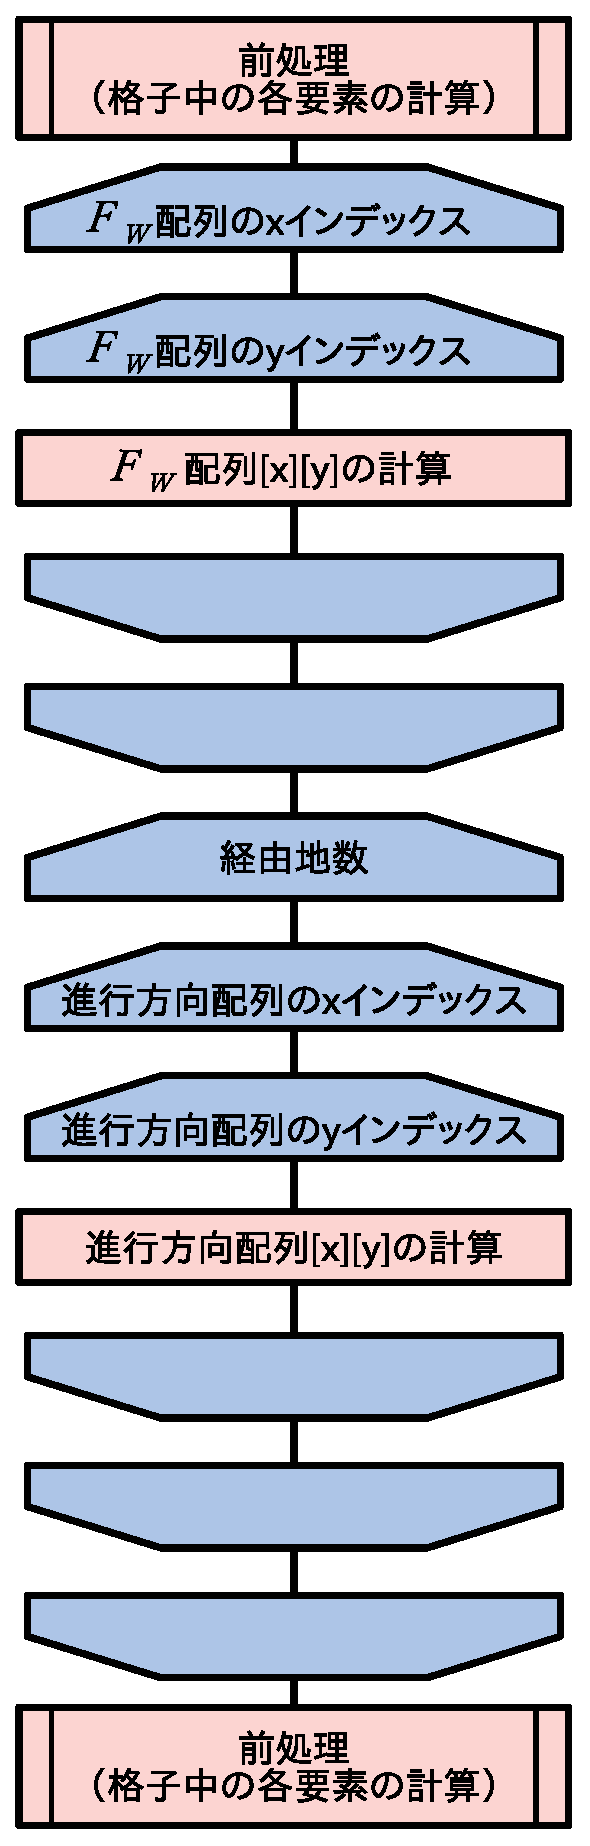
\includegraphics[width=4.5cm,clip]{figure/5_teian_flow2.eps}
  \caption{格子分割の前処理のフローチャート}
  \label{fig:5_teian_flow2}
 \end{center}
\end{figure}

\clearpage
\subsection{個別に進行方向を計算する格子の判定}
格子分割を用いた進行方向の計算回数削減手法は,精度の大幅な低下を防ぐために,
\figref{fig:ex2}のように目的地や障害物が含まれる格子とその周辺の格子に存在するエージェントを
個別に進行方向を計算するように設定する.
個別に進行方向する格子には,xとyの両方のベクトルに0が格納されているため,
解析中にエージェントが存在する格子に0ベクトルが格納されているか判定が必要となる.
\figref{fig:5_teian_flow2}に進行方向ベクトル$e$および障害物を避ける力$F_{iW}$の
解析中に個別計算するかどうかの判定のフローチャートを示す.
\figref{fig:5_teian_flow2}が示すフローチャートは,\figref{fig:5_teian_flow1}中の
解析中の運動方程式を用いた計算であり,エージェントの進行方向を求めるための計算である.
\figref{fig:5_teian_flow2}中の$F_{iW}$配列は障害物を避ける力$F_{iW}$を格納する配列,
進行方向配列は進行方向ベクトル$e$を格納する配列である.
\figref{fig:5_teian_flow2}に示すように,格子分割を用いた進行方向の計算回数削減手法は,
エージェントの座標から参照する配列の要素を求め,0ベクトルが格納されていない場合に
配列中の値を参照し,0ベクトルが格納されている場合に個別計算を行うことで解析中の
計算回数を削減する.

\textbf{(周辺にも0ベクトルを入れることを書く)}


\figtb{提案手法の運動方程式計算のフローチャート}{}{9}{5_teian_flow3.eps}{5_teian_flow2}
%\figtb{シミュレーション中の$f_{iW}$計算のフローチャート}{}{8.5}{5_e_flow.eps}{5_e_flow}


\clearpage
\section{評価}
SFMを用いた人流シミュレーションに対する
格子分割を用いた進行方向の計算回数削減手法の有効性を確認するために,
既存手法であるセル分割法と提案手法を用いて人流シミュレーション
評価環境は,\tabref{tb:result_env}に示すマシンである.
本評価では,\tabref{tb:result_para}に示すパラメータを用いて
SFMの運動方程式を計算する.
本評価では,避難時のシミュレーションを再現するために,
エージェント数よりも壁粒子が多い配置にエージェントを一方向に進むような解析を行う.
\figref{fig:5_initialconf}に本評価に用いるエージェントの初期配置を示す.
\figref{fig:5_initialconf}中の黄色の四角は障害物(壁),赤色のひし形は目的地,
緑色の四角はエージェントの初期配置位置である.
\figref{fig:5_initialconf}のエージェントは,緑色の範囲内から赤色の目的地まで
進むように設定する.本評価では,格子サイズごとの計算回数の削減率や,解析時間の
有効性を評価するために,\figref{fig:5_initialconf}に示す配置の壁の間隔や粒子数を変えた
複数パターンを用いる.
\figref{fig:haba2}と\figref{fig:haba5},\figref{fig:haba10},\figref{fig:haba20}に
評価で用いる\figref{fig:5_initialconf}のエージェントの初期配置の壁間隔を変えた配置を示す.
また,\figref{fig:haba2_2},\figref{fig:haba2_3}に通路幅2mのときの配置(\figref{fig:haba2})
の壁粒子をそれぞれ2倍,3倍にした配置を示す.
図中の黒丸は壁粒子,紫色の丸はエージェント,青色の丸は目的地である.
図に示す配置のエージェントは40人,壁粒子は592個,経由地は1個,
解析領域は$50m \times 50m$である.
また,壁粒子を変えた配置(\figref{fig:haba2_2},\figref{fig:haba2_3})の
壁粒子数は\tabref{tb:haba_atusa}に示す通りである.
図中のすべてのエージェントは,青色の丸が示す目的地に向かうように設定する.
測定する格子サイズは,解析領域の一辺(50m)を半分ずつ割った値を用いる.

\begin{table}[t]
  \begin{center}
    \caption{評価環境}
      \label{tb:result_env}
      \begin{tabular}{c|c}
      \hline \hline
      CPU              & Intel Xeon CPU E5-2667w v2 \\ \hline
      メモリ           & 32GB                       \\ \hline
      OS               & Linux 6.5.8               \\ \hline
      コンパイラ       & gcc 13.2.0                  \\ \hline
      最適化オプション & -O3                        \\ \hline
    \end{tabular}
  \end{center}
\end{table}

\begin{table}[t]
  \begin{center}
    \caption{測定条件}
    \label{tb:result_para}
    \begin{tabular}{c|c}
      \hline \hline
      $A_i$            & 2000N                              \\ \hline 
      $B_i$            & 0.08m                              \\ \hline 
      $k$              & $1.2 \times 10^5 kg s^{-2} $       \\ \hline 
      $\kappa$         & $2.4 \times 10^5 kg m^{-1} s^{-2}$ \\ \hline 
      $v_i^0$          & $1.4$m/s                           \\ \hline 
      $m_i$            & $80$kg                             \\ \hline 
      $\tau_i$         & 0.5                               \\ \hline 
      $r_i$            & $0.25$m                            \\ \hline 
      相互作用範囲     & $5$m                              \\ \hline 
    \end{tabular}
  \end{center}
\end{table}


\begin{table}
  \begin{center}
    \caption{壁の厚さを変えたときの初期配置のパラメータ}
    \label{tb:haba_atusa}
    \begin{tabular}{c|c|c|c}
      \hline \hline
            & 壁粒子数[個] & エージェント数[人] & 経由地数[個] \\ \hline
      厚さ1倍 & 592  & 40 & 1 \\ \hline
      厚さ2倍 & 1184 & 40 & 1 \\ \hline
      厚さ3倍 & 1776 & 40 & 1 \\ \hline
    \end{tabular}
  \end{center}
\end{table}


\figtb{エージェントの初期配置}{}{11}{5_initialconfiguration.eps}{5_initialconf}

\clearpage

\dfig{通路幅2mの初期配置}{20231023_haba2}{haba2}{通路幅5mの初期配置}{20231023_haba5}{haba5}

\dfig{通路幅10mの初期配置}{20231023_haba10}{haba10}{通路幅20mの初期配置}{20231023_haba20}{haba20}

\dfig{通路幅2m(壁粒子数2倍)の初期配置}{haba2_2}{haba2_2}{通路幅2m(壁粒子数3倍)の初期配置}{haba2_3}{haba2_3}

\clearpage


%result figure {{{
\begin{figure}[tb]
	\begin{minipage}[b]{0.48\columnwidth}
		\begin{center}
		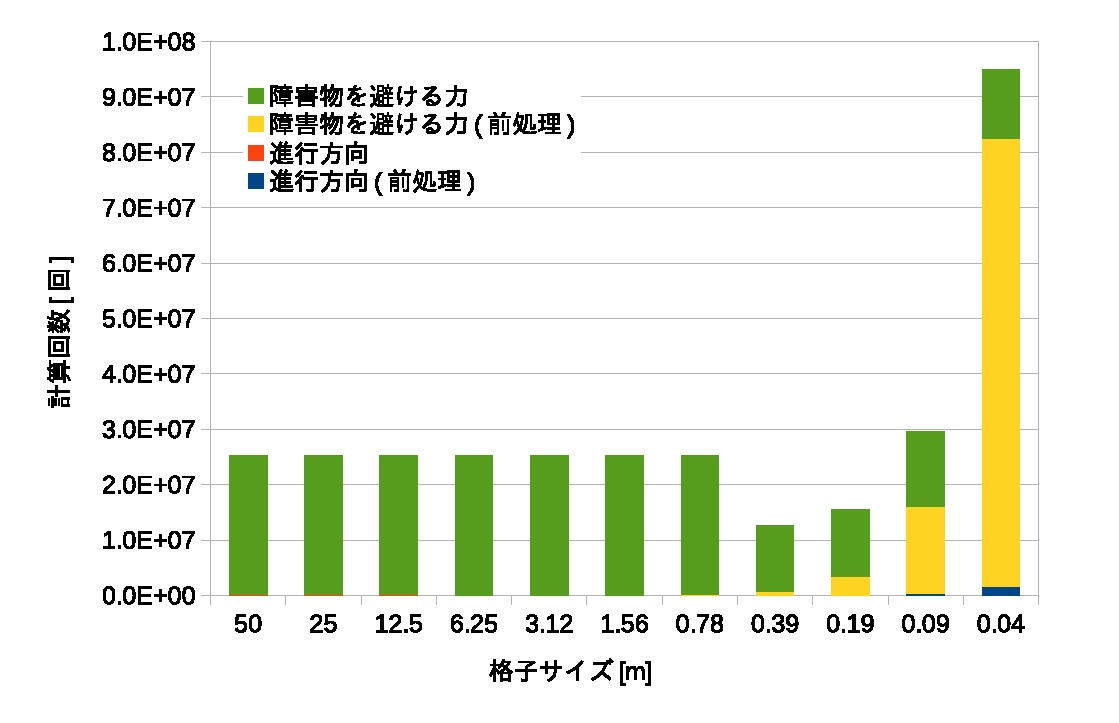
\includegraphics[width=\columnwidth]{figure/5_result_2m_times.eps}
		\caption{通路幅2mの格子サイズごとの計算回数}
		\label{fig:result_2m_times}
		\end{center}
	\end{minipage}
	\hspace{0.04\columnwidth}
	\begin{minipage}[b]{0.48\columnwidth}
		\begin{center}
		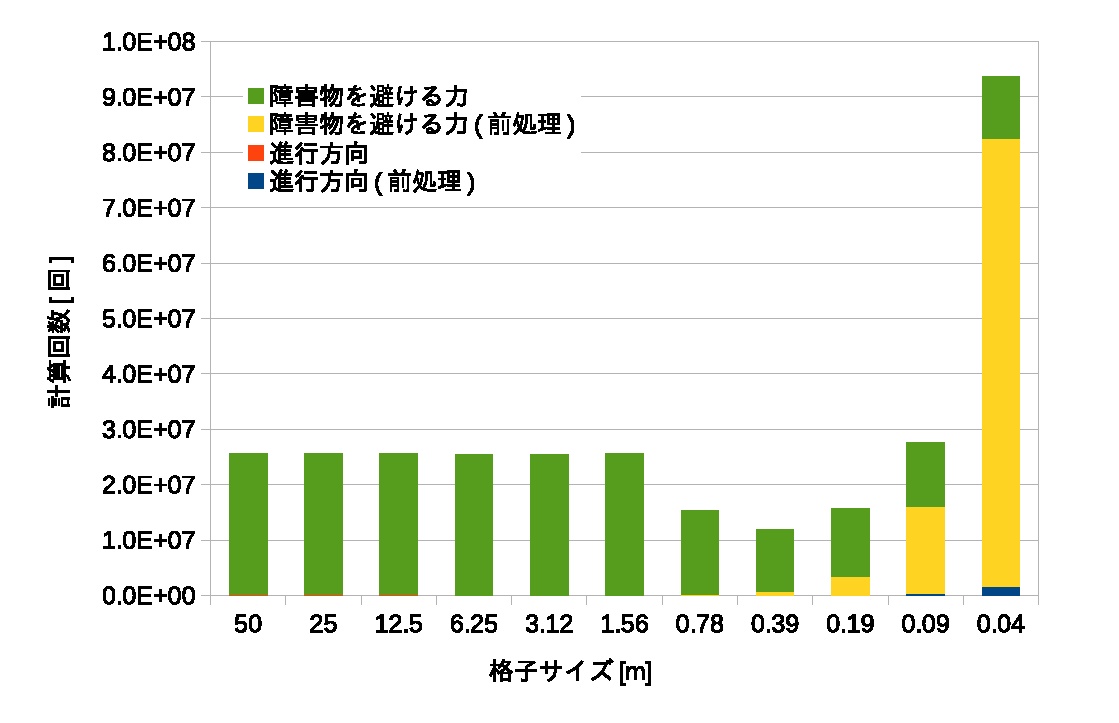
\includegraphics[width=\columnwidth]{figure/5_result_5m_times.eps}
		\caption{通路幅5mの格子サイズごとの計算回数}
		\label{fig:result_5m_times}
		\end{center}
	\end{minipage}
\end{figure}
%}}}
%result figure {{{
\begin{figure}[tb]
	\begin{minipage}[b]{0.48\columnwidth}
		\begin{center}
		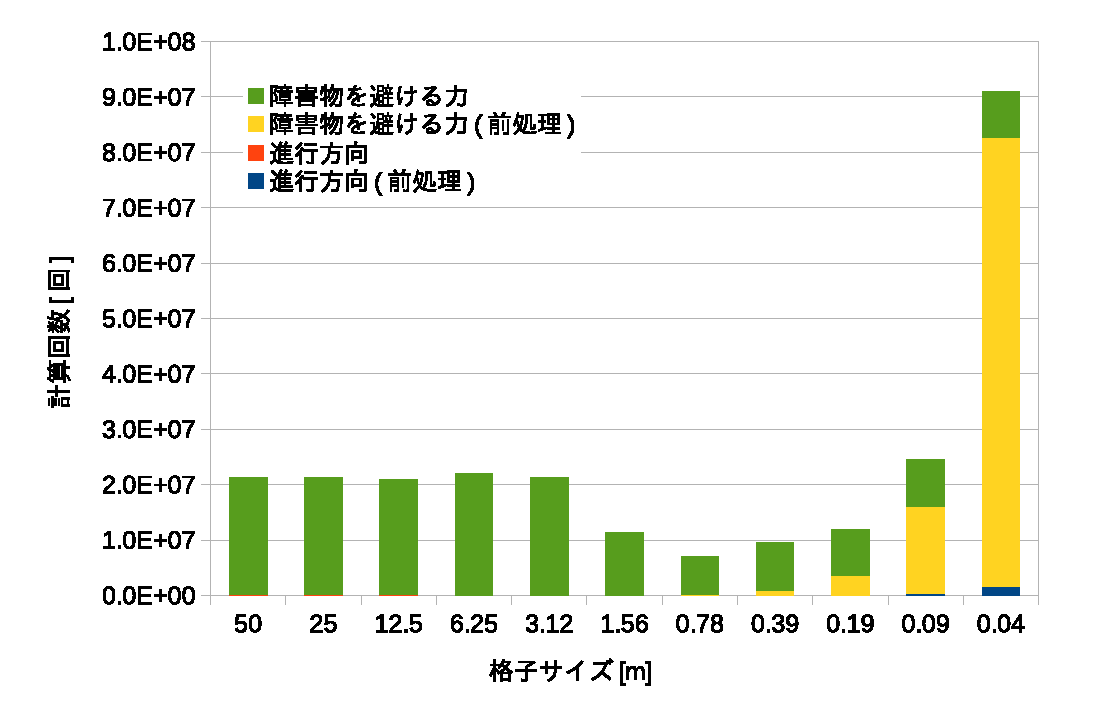
\includegraphics[width=\columnwidth]{figure/5_result_10m_times.eps}
		\caption{通路幅10mの格子サイズごとの計算回数}
		\label{fig:result_10m_times}
		\end{center}
	\end{minipage}
	\hspace{0.04\columnwidth}
	\begin{minipage}[b]{0.48\columnwidth}
		\begin{center}
		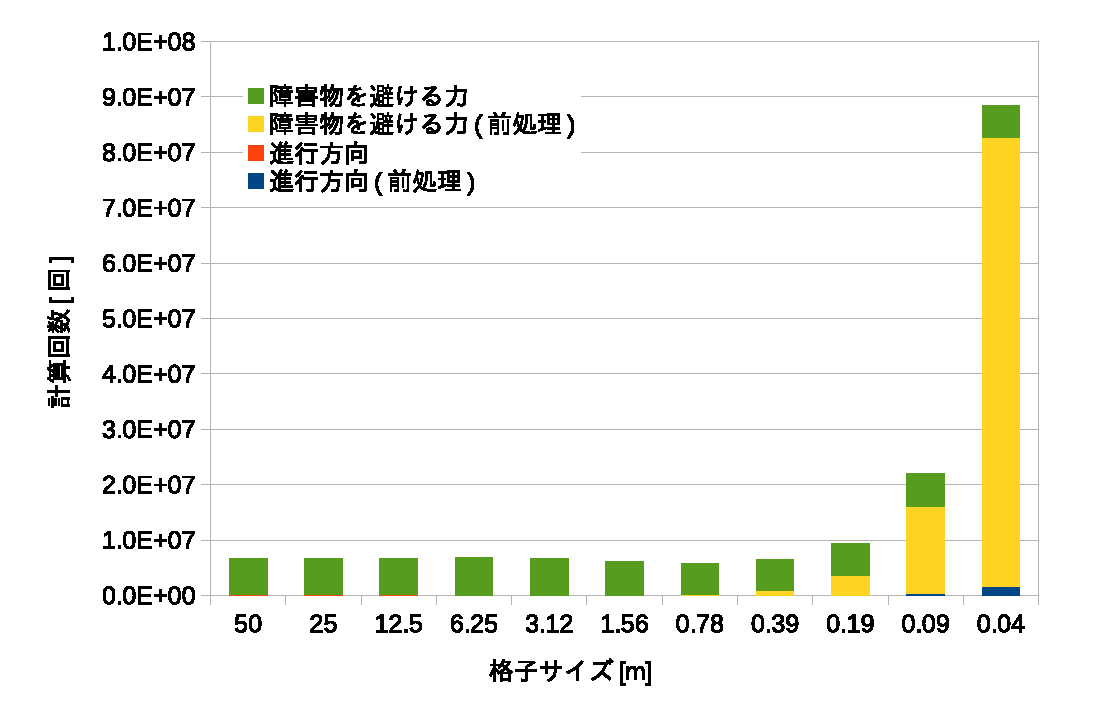
\includegraphics[width=\columnwidth]{figure/5_result_20m_times.eps}
		\caption{通路幅20mの格子サイズごとの計算回数}
		\label{fig:result_20m_times}
		\end{center}
	\end{minipage}
\end{figure}
%}}}

%削減率の表{{{
\begin{table}[tb]
  \centering
  \caption{各通路幅の格子サイズごとの計算回数の削減率[\%]}
  \label{tb:5_times_sakugenritu}
    \begin{tabular}{r|r|r|r|r}
    \hline \hline
              & 通路幅2m       & 通路幅5m       & 通路幅10m      & 通路幅20m     \\ \hline
        50.00 & 0.00           & 0.00           & 0.00           & 0.00          \\ \hline
        25.00 & 0.00           & 0.00           & 0.00           & 0.00          \\ \hline
        12.50 & 0.08           & 0.07           & 1.03           & 0.03          \\ \hline
        6.25  & 0.23           & 0.25           & -3.04          & -0.93         \\ \hline
        3.12  & 0.15           & 0.22           & -0.12          & 1.57          \\ \hline
        1.56  & 0.19           & 0.10           & 37.69          & 6.44          \\ \hline
        0.78  & 0.50           & 33.86          & \textbf{54.81} & \textbf{8.25} \\ \hline
        0.39  & \textbf{43.85} & \textbf{45.48} & 44.98          & 1.60          \\ \hline
        0.19  & 34.61          & 32.68          & 35.66          & -23.33        \\ \hline
        0.09  & -13.93         & -6.88          & -12.48         & -137.22       \\ \hline
        0.04  & -235.83        & -225.08        & -267.49        & -738.82       \\ \hline
    \end{tabular}
\end{table}
%}}}

\subsection{進行方向計算の計算回数(工事中)}
\label{sec:5_calc_times}
本測定では,格子分割を用いた進行方向の計算回数削減手法の
有効性を評価するために,既存手法であるセル分割法と
格子分割を用いた進行方向の計算回数削減手法の計算回数を測定する.
測定する計算は,エージェントの進行方向の決定に必要な
エージェントの進行方向ベクトル$e$と
障害物を避ける力$F_{iW}$であり,前処理と解析中の回数である.
\figref{fig:result_2m_times},\figref{fig:result_5m_times},
\figref{fig:result_10m_times},\figref{fig:result_20m_times}に
各配置における計算回数を示す.
また,\tabref{tb:5_times_sakugenritu}に各配置における削減率を示す.
\tabref{tb:5_times_sakugenritu}に示す削減率は,式\eqref{eq:5_sakugenritu}
のように,セル分割法の各計算の総和$C_e$と提案手法の各計算の総和$C_p$を
用いて算出する.
%
\begin{eqnarray}
\mbox{削減率[\%]} = \Big ( 1 - \frac{C_p}{C_e}  \Big) \times 100
\label{eq:5_sakugenritu}
\end{eqnarray}
%

\figref{fig:result_2m_times}から\figref{fig:result_20m_times}より,
提案手法は,セル分割法よりも進行方向の計算回数が削減できる格子サイズが
あることが確認できる.
また,すべての配置において格子サイズが小さくなるほど,前処理の計算が
占める割合が高くなることがわかる.
これは,格子サイズが小さくなるほど,あらかじめ計算する進行方向を保持する
格子の要素数が多くなるため,前処理の計算回数が増えるためであると考えられる.
一方で,進行方向ベクトル$e$の計算は,各計算回数に対しての割合が低い.
これは,解析中の進行方向ベクトル$e$の計算回数が最大で
エージェント数とタイムステップ数の積であることから,障害物を避ける力の
計算回数よりも低いためであると考えられる.
%
\tabref{tb:5_times_sakugenritu}より,
提案手法がセル分割法に対して計算回数が削減できる格子サイズは,
通路幅2mで0.39mから0.19m,
通路幅5mで0.78mから0.19m,
通路幅10mで1.56mから0.19m,
通路幅20mで3.12mから0.78mであり,
通路幅が広くなるほど削減できる格子サイズの大きさが大きくなる.
これは,通路幅が広くなるほど,エージェントが通る場所の格子内に
壁粒子が含まれにくくなるため,あらかじめ計算した進行方向を
用いることができるからであると考えれれる.
[\textbf{炭治郎柄の図を使って説明しても良い}]
%
各通路幅の削減率は,\tabref{tb:5_times_sakugenritu}より,通路幅2mで最大43.85\%,
通路幅5mで最大45.48\%,通路幅10mで最大54.81\%,通路幅20mで最大8.25\%である.
通路幅20mの最大の削減率は,最大約8\%であり,他の通路幅の最大削減率(約50\%前後)と
比べて低いことがわかる.
これは,\figref{fig:result_2m_times}から\figref{fig:result_20m_times}より,
通路幅2mから10mのセル分割法の計算回数が約2000万回から約3000万回の間であるのに対して,
通路幅20mのときのセル分割法の計算回数が約500万回であり,
通路幅20mの計算回数が少なく,削減率が低くなったためであると考えられる.
また,
通路幅20mにおける既存手法の計算回数が少ない理由は,本評価で用いたパラメータの
影響範囲が5mであり,\figref{fig:haba20}に示すように,エージェントが通る場所が
通路幅20mであるため,エージェントの障害物を避ける力の影響範囲に壁粒子が存在しない
ことが多く,障害物を避ける力の計算回数が他の通路幅と比べて少ない結果が得られたと
考えられる.
%
\figref{fig:result_5m_times}から\figref{fig:result_20m_times}より,
前処理中の計算回数が占める割合は,どの通路幅の配置においても同様の傾向である結果が得られた.
これは,本評価に用いる配置の経由地数と解析領域が同じであるため,
式\eqref{eq:route_youso_size}や式\eqref{eq:fiw_youso_size}に示す前処理に必要な要素数が同じであり,
壁粒子数が同じであることから,通路幅が変わっても同様の傾向が得られたと考えられる.


%result figure {{{
\begin{figure}[tb]
	\begin{minipage}[b]{0.48\columnwidth}
		\begin{center}
		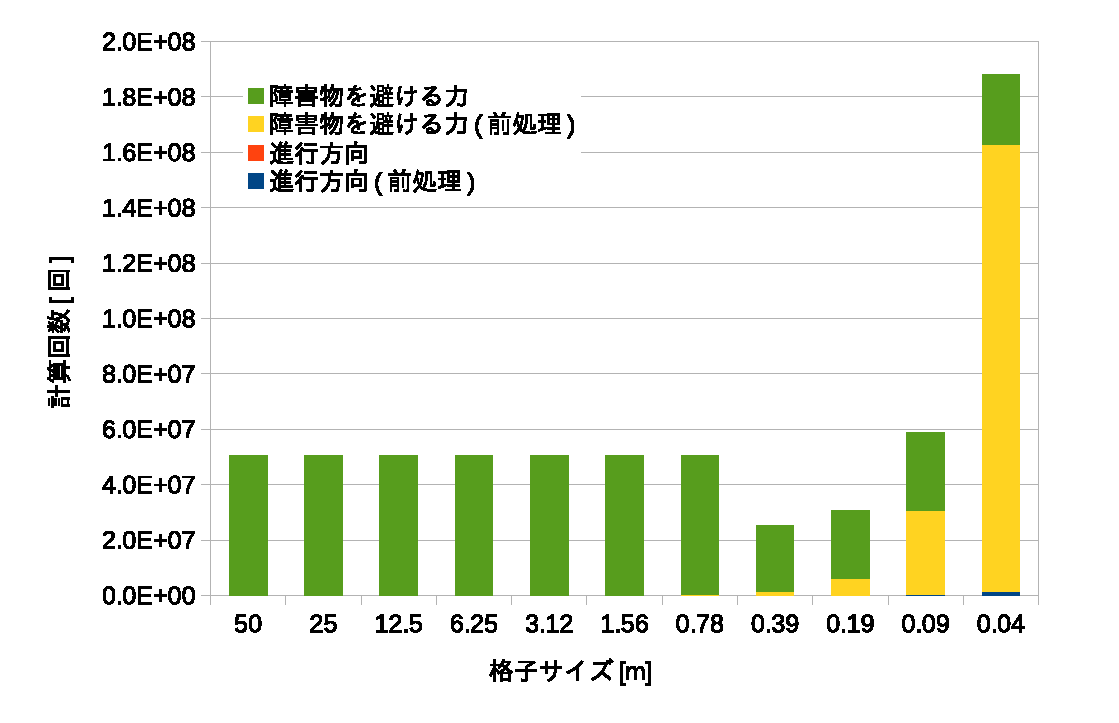
\includegraphics[width=\columnwidth]{figure/5_result_2bai_times.eps}
		\caption{通路幅2m(壁粒子2倍)の格子サイズごとの計算回数}
		\label{fig:result_2bai_times}
		\end{center}
	\end{minipage}
	\hspace{0.04\columnwidth}
	\begin{minipage}[b]{0.48\columnwidth}
		\begin{center}
		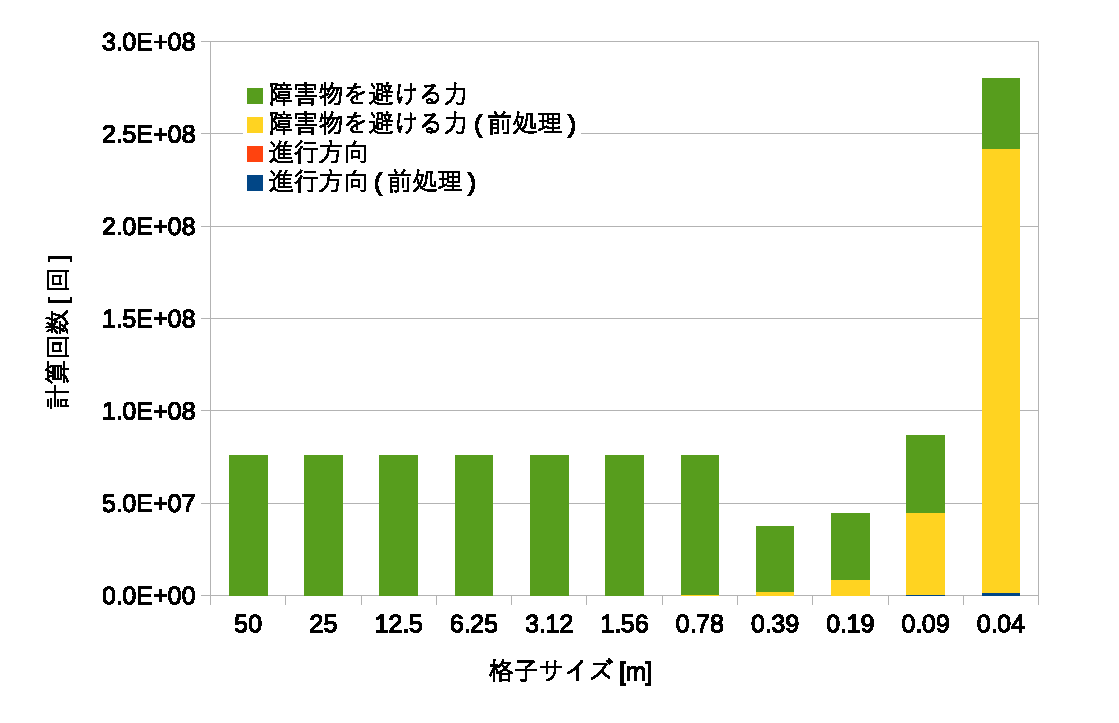
\includegraphics[width=\columnwidth]{figure/5_result_3bai_times.eps}
		\caption{通路幅2m(壁粒子3倍)の格子サイズごとの計算回数}
		\label{fig:result_3bai_times}
		\end{center}
	\end{minipage}
\end{figure}
%}}}
%昔の図{{{
%\figtb{通路幅2mの計算回数}{}{11}{5_result_2m_times.eps}{result_2m_times}
%\figtb{通路幅5mの計算回数}{}{11}{5_result_5m_times.eps}{result_5m_times}
%\figtb{通路幅10mの計算回数}{}{11}{5_result_10m_times.eps}{result_10m_times}
%\figtb{通路幅20mの計算回数}{}{11}{5_result_20m_times.eps}{result_20m_times}
%
%\figtb{通路幅2m(壁粒子2倍)の計算回数}{}{11}{5_result_2bai_times.eps}{result_2bai_times}
%\figtb{通路幅2m(壁粒子3倍)の計算回数(仮画像)}{}{11}{5_result_2bai_times.eps}{result_2bai_times}
%}}}
%削減率の表{{{
\begin{table}[tb]
  \centering
  \caption{各通路幅の格子サイズごとの計算回数の削減率[\%]}
  \label{tb:5_times_sakugenritu}
    \begin{tabular}{r|r|r|r|r}
    \hline \hline
              & 通路幅2m       & 通路幅5m       & 通路幅10m      & 通路幅20m     \\ \hline
        50.00 & 0.00           & 0.00           & 0.00           & 0.00          \\ \hline
        25.00 & 0.00           & 0.00           & 0.00           & 0.00          \\ \hline
        12.50 & 0.08           & 0.07           & 1.03           & 0.03          \\ \hline
        6.25  & 0.23           & 0.25           & -3.04          & -0.93         \\ \hline
        3.12  & 0.15           & 0.22           & -0.12          & 1.57          \\ \hline
        1.56  & 0.19           & 0.10           & 37.69          & 6.44          \\ \hline
        0.78  & 0.50           & 33.86          & \textbf{54.81} & \textbf{8.25} \\ \hline
        0.39  & \textbf{43.85} & \textbf{45.48} & 44.98          & 1.60          \\ \hline
        0.19  & 34.61          & 32.68          & 35.66          & -23.33        \\ \hline
        0.09  & -13.93         & -6.88          & -12.48         & -137.22       \\ \hline
        0.04  & -235.83        & -225.08        & -267.49        & -738.82       \\ \hline
    \end{tabular}
\end{table}
%}}}

%壁粒子数を変えたときの削減率{{{
\begin{table}[tb]
  \centering
  \caption{各通路幅の格子サイズごとの計算回数の削減率[\%]}
  \label{tb:5_bai_sakugenritu}
    \begin{tabular}{r|r|r|r}
    \hline \hline
		      & 壁粒子(1倍)    & 壁粒子(2倍)      & 壁粒子(3倍)        \\ \hline
		50.00 & 0.00           & 0.00             & 0.00               \\ \hline
		25.00 & 0.00           & 0.00             & 0.00               \\ \hline
		12.50 & 0.08           & 0.00             & 0.03               \\ \hline
		 6.25 & 0.23           & 0.03             & 0.08               \\ \hline
		 3.12 & 0.15           & 0.02             & 0.00               \\ \hline
		 1.56 & 0.19           & 0.05             & 0.11               \\ \hline
		 0.78 & 0.50           & 0.21             & 0.29               \\ \hline
		 0.39 & \textbf{43.85} & \textbf{47.00}   & \textbf{48.46}     \\ \hline
		 0.19 & 34.61          & 36.81            & 39.93              \\ \hline
		 0.09 & -13.93         & -14.68           & -13.39             \\ \hline
		 0.04 & -235.83        & -251.21          & -255.13            \\ \hline
    \end{tabular}
\end{table}
%}}}

\figref{fig:result_2bai_times},\figref{fig:result_3bai_times}より,
提案手法は,壁粒子数が増加した場合においても\figref{fig:result_2m_times}と同様に
格子サイズ0.39mから0.19mの間で削減できることが確認できる.
\figref{fig:result_2bai_times},\figref{fig:result_3bai_times}の結果から式\eqref{eq:5_sakugenritu}
を用いて算出した各配置の削減率を\tabref{tb:5_bai_sakugenritu}に示す.
\tabref{tb:5_bai_sakugenritu}中の太字の数値は,各配置の削減率の最大値を示す.
\tabref{tb:5_bai_sakugenritu}より,壁粒子数が多くなるほど,計算回数の削減率の最大値が高くなることがわかる.
これは,壁粒子の密度が高くなるほど,既存手法であるセル分割法の計算回数が増加するため,提案手法の
削減できる計算回数が多くなるためであると考えられる.

以上のことから,提案手法は,〜〜〜である(このサブセクションの総括).

\clearpage
\subsection{シミュレーションの実行時間の測定}
\label{sec:5_calc_jikan}
\ref{sec:5_calc_times}節より,提案手法を用いることで,既存手法であるセル分割法よりも
進行方向の計算回数を削減できることが確認できた.
一方で,提案手法は,解析前にあらかじめ各格子の進行方向を計算するため,解析前の前処理の
実行時間は増加する.このため,あらかじめ計算するために必要な時間を考慮しても
格子分割を用いた進行方向の計算回数削減による高速化が有効であることを確認する.
\figref{fig:result_2m_jikan},\figref{fig:result_5m_jikan},
\figref{fig:result_10m_jikan},\figref{fig:result_20m_jikan}に通路幅ごとの
シミュレーション実行時間を,\figref{fig:5_kousokuka_haba}に式\eqref{eq:5_kousokuka}を用いて算出した
高速化率を示す.
また,\figref{fig:result_2bai_jikan},\figref{fig:result_3bai_jikan}に通路幅2mのときの
粒子数を2倍,3倍にした配置のシミュレーション実行時間を,\figref{fig:5_kousokuka_atusa}に高速化率を示す.
%
\begin{align}
	\mbox{高速化率[倍]} = \frac{\mbox{セル分割法の実行時間[s]}}
    {\mbox{提案手法の実行時間[s]}}
    \label{eq:5_kousokuka}
\end{align}
%
\figref{fig:result_2m_jikan},\figref{fig:result_5m_jikan},
\figref{fig:result_10m_jikan},\figref{fig:result_20m_jikan},
\figref{fig:5_kousokuka_haba}より,
提案手法は,セル分割法よりも最大△△倍高速であり,
従来手法よりも解析時間が最大○○割削減できることが確認できる.
また,格子サイズが小さくなるほど,前処理の計算にかかる時間の
割合が多くなり,通路幅2mでは0.09m,通路幅5mでは0.09m,通路幅10mでは
0.19m,通路幅20mでは0.39m以下の格子サイズで,従来手法よりも
遅くなることが確認できる.
前処理時間にかかる時間は,\ref{sec:5_calc_times}節で示した
前処理中の計算回数が占める割合の傾向と同様であることがわかる.
従来手法よりも高速に解析できる提案手法の格子サイズは,
通路幅2mで0.39mから0.19m,
通路幅5mで0.78mから0.19m,
通路幅10mで1.56mから0.19m,
通路幅20mで6.25mから0.39mであり,
通路幅が広くなるほど,従来手法よりも高速に解析できる格子サイズが
多くなることがわかる.
これをふまえると,従来手法よりも高速に解析できる提案手法の
格子サイズは,エージェントが通る場所の障害物と障害物の間の距離に
応じて変わることが考えられる.
\textbf{[壁粒子数を変えた時のシミュレーション実行時間と高速化率
について述べる!!!]} 

\figref{fig:result_2bai_jikan},\figref{fig:result_3bai_jikan},
\figref{fig:5_kousokuka_atusa}より,
提案手法のセル分割法に対する高速化率は,
壁粒子数1倍のときで最大○○倍,
壁粒子数2倍のときで最大○○倍,
壁粒子数3倍のときで最大○○倍であり,
壁粒子数が増えるほど高速化率の最大値が高くなることが確認できる.
これは,壁粒子を増やす方法が壁粒子の密度が高くなるような設定をしているため,
密度が高くなるほど,\ref{sec:5_calc_times}節で示した計算回数が削減でき,
解析時間の短縮に繋がったと考えられる.



\begin{figure}[tb]
	\begin{minipage}[b]{0.48\columnwidth}
		\begin{center}
		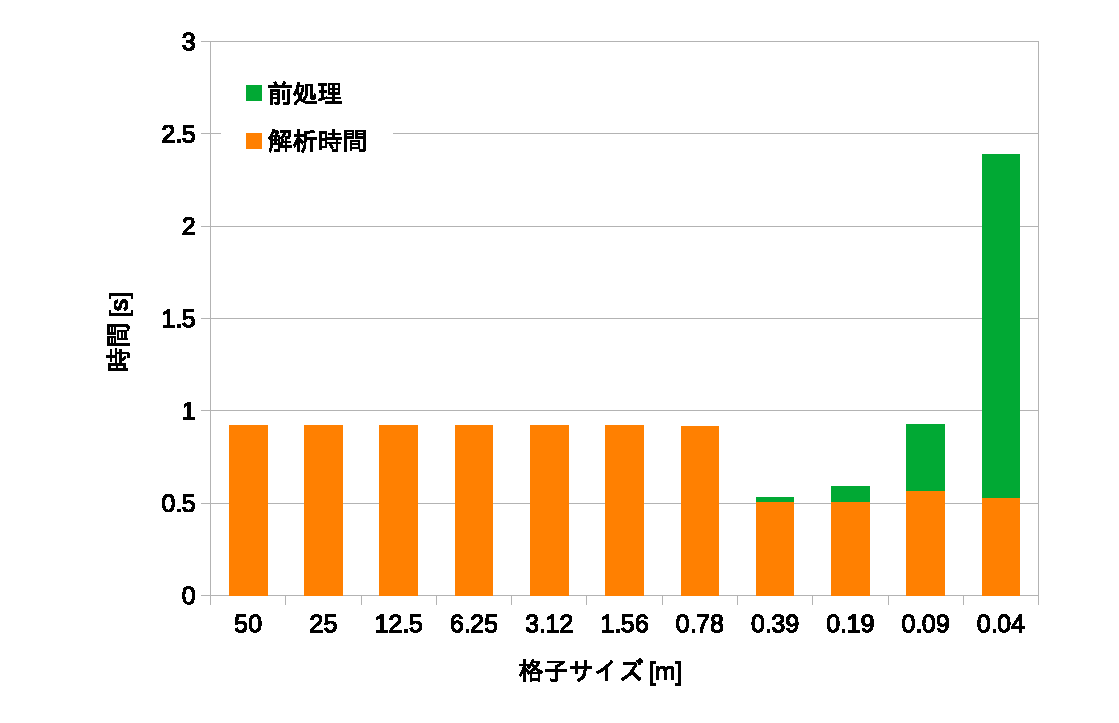
\includegraphics[width=\columnwidth]{figure/5_2m_jikan.eps}
		\caption{通路幅2mの格子サイズごとの解析時間}
		\label{fig:result_2m_jikan}
		\end{center}
	\end{minipage}
	\hspace{0.04\columnwidth}
	\begin{minipage}[b]{0.48\columnwidth}
		\begin{center}
		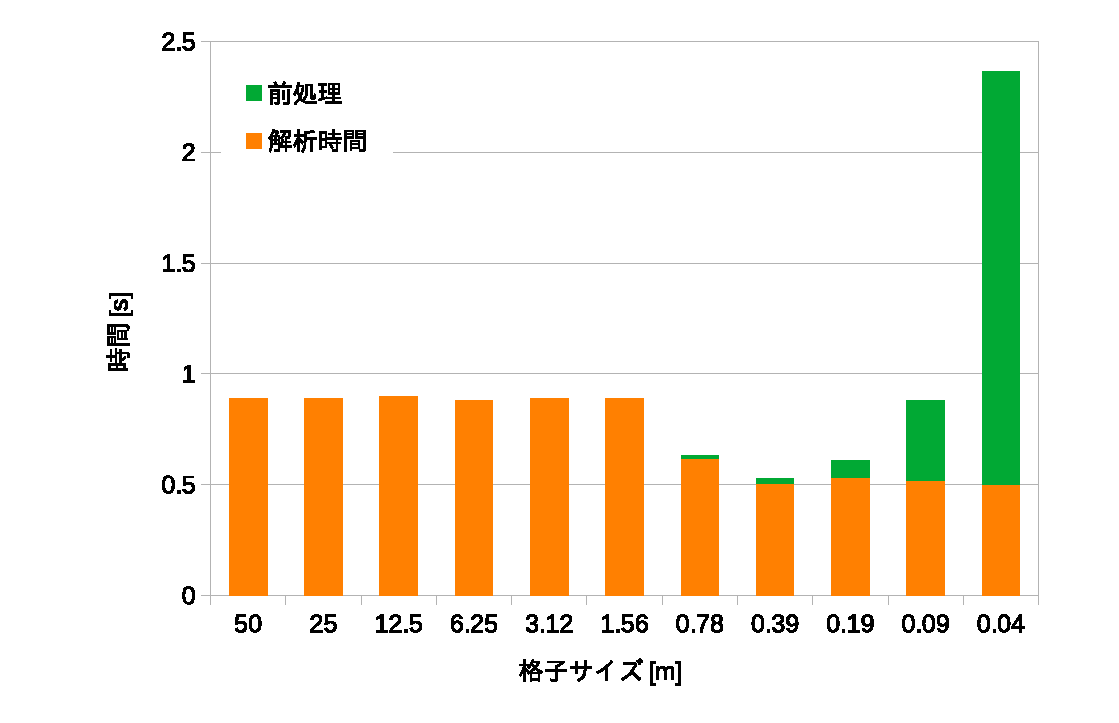
\includegraphics[width=\columnwidth]{figure/5_5m_jikan.eps}
		\caption{通路幅5mの格子サイズごとの解析時間}
		\label{fig:result_5m_jikan}
		\end{center}
	\end{minipage}
\end{figure}

\begin{figure}[tb]
	\begin{minipage}[b]{0.48\columnwidth}
		\begin{center}
		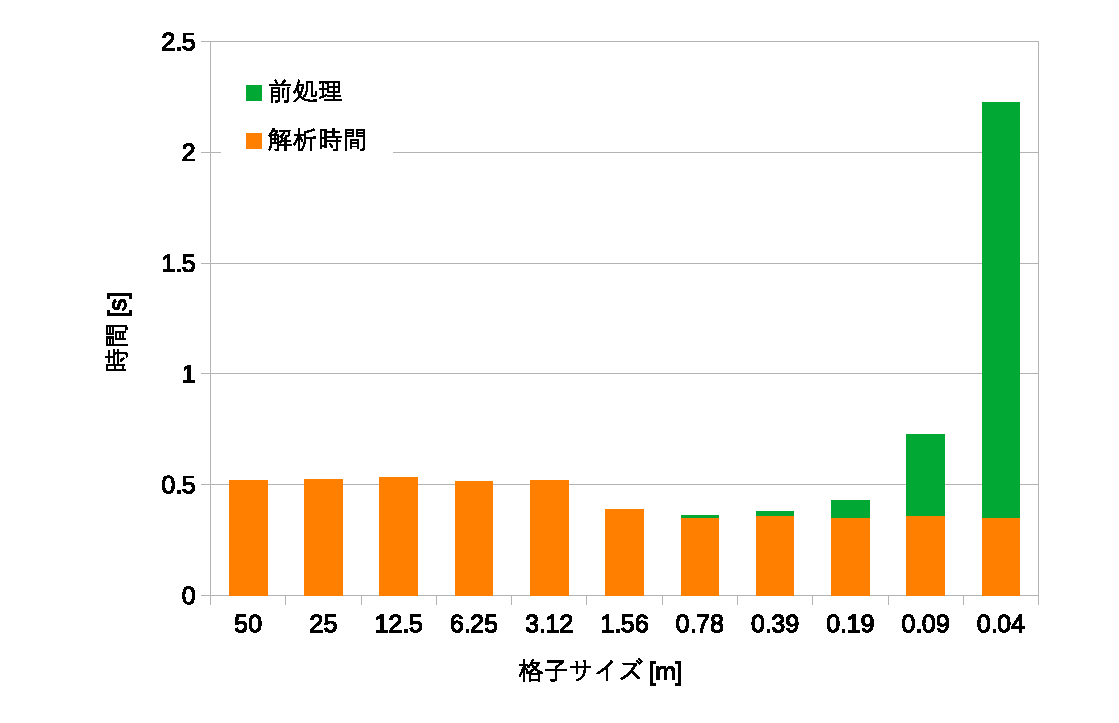
\includegraphics[width=\columnwidth]{figure/5_10m_jikan.eps}
		\caption{通路幅10mの格子サイズごとの解析時間}
		\label{fig:result_10m_jikan}
		\end{center}
	\end{minipage}
	\hspace{0.04\columnwidth}
	\begin{minipage}[b]{0.48\columnwidth}
		\begin{center}
		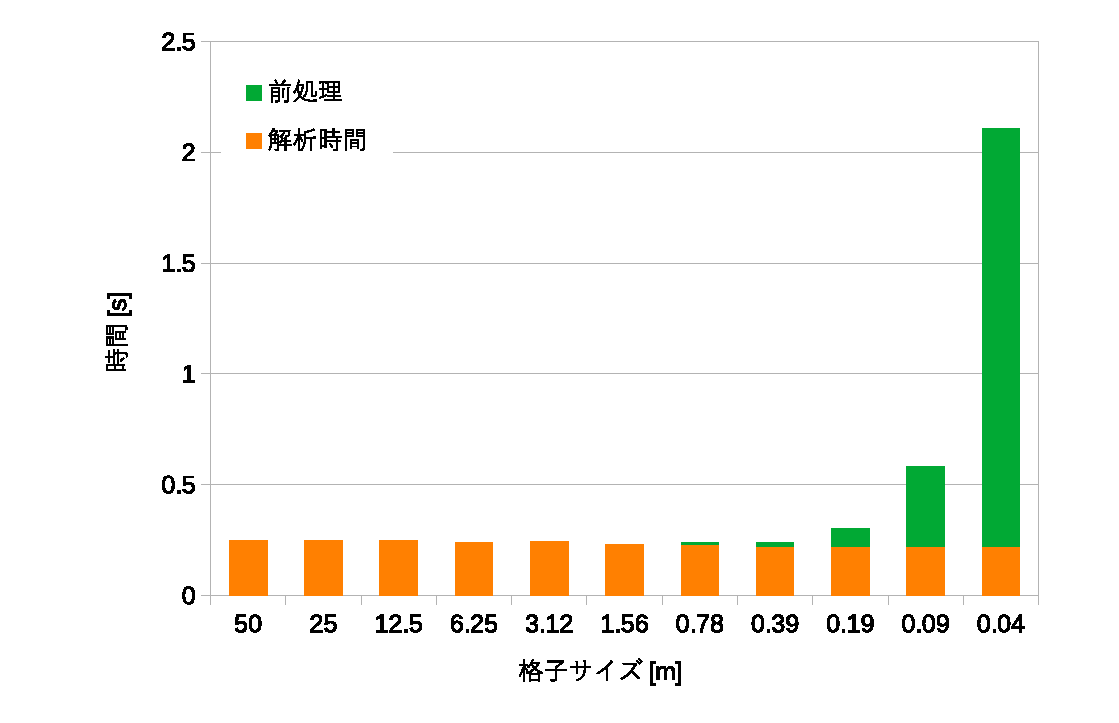
\includegraphics[width=\columnwidth]{figure/5_20m_jikan.eps}
		\caption{通路幅20mの格子サイズごとの解析時間}
		\label{fig:result_20m_jikan}
		\end{center}
	\end{minipage}
\end{figure}

\begin{figure}[tb]
	\begin{minipage}[b]{0.48\columnwidth}
		\begin{center}
		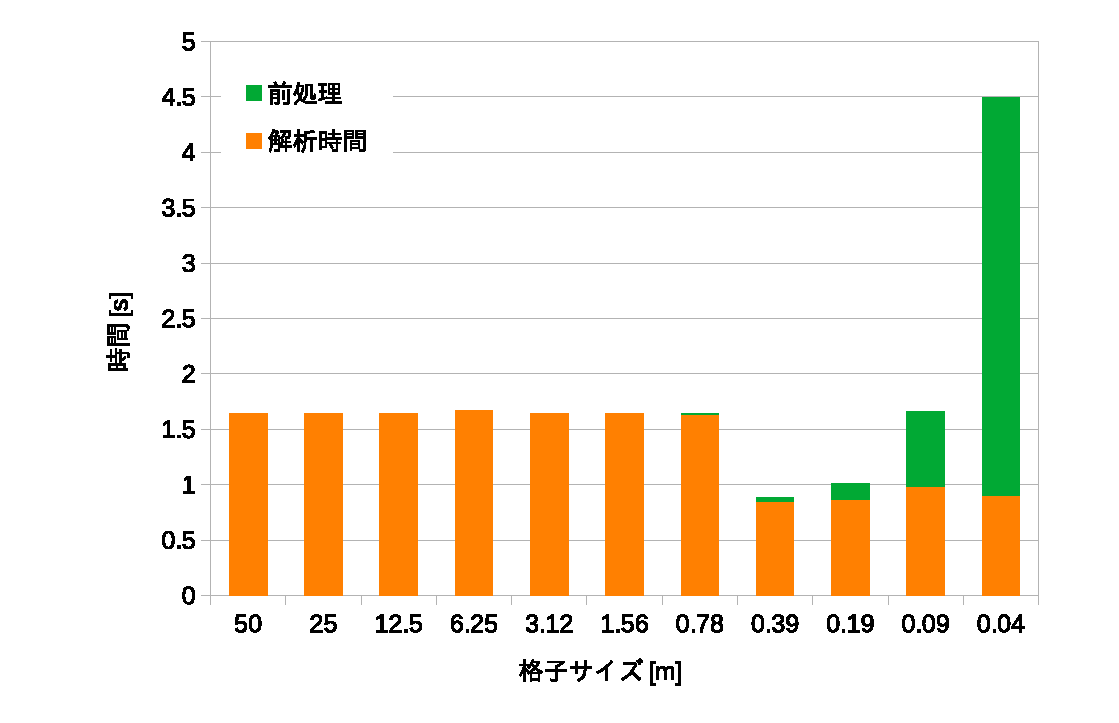
\includegraphics[width=\columnwidth]{figure/5_2bai_jikan.eps}
		\caption{通路幅2m(粒子数2倍)の格子サイズごとの解析時間}
		\label{fig:result_2bai_jikan}
		\end{center}
	\end{minipage}
	\hspace{0.04\columnwidth}
	\begin{minipage}[b]{0.48\columnwidth}
		\begin{center}
		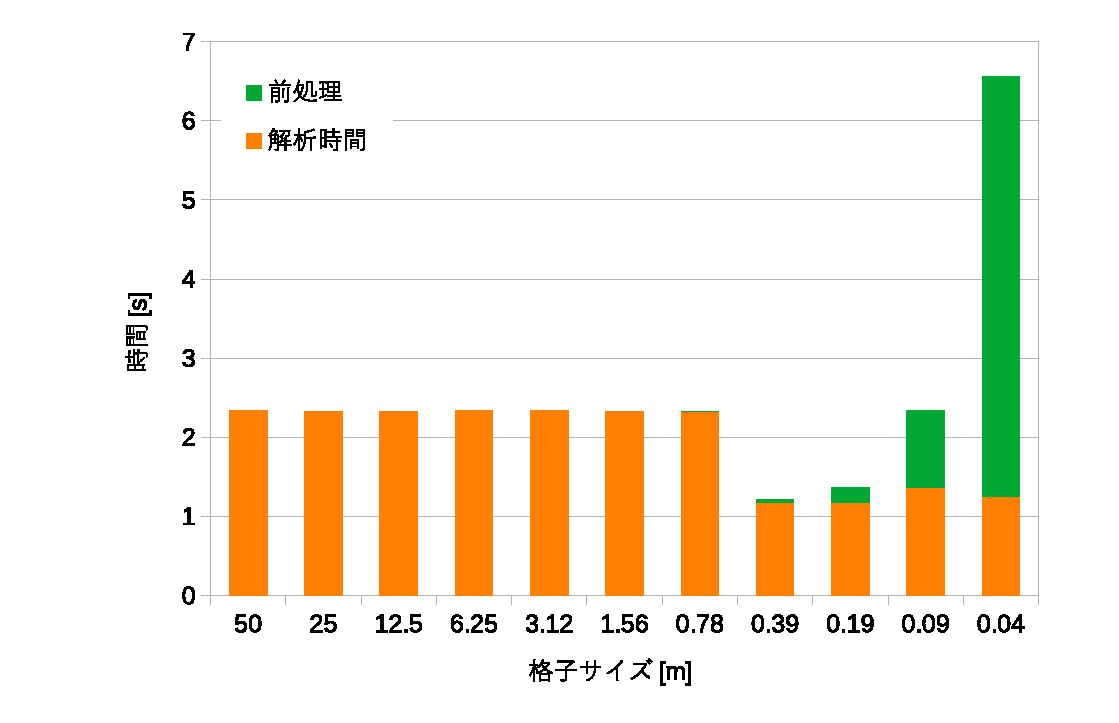
\includegraphics[width=\columnwidth]{figure/5_3bai_jikan.eps}
		\caption{通路幅3m(粒子数3倍)の格子サイズごとの解析時間}
		\label{fig:result_3bai_jikan}
		\end{center}
	\end{minipage}
\end{figure}


\begin{figure}[tb]
 \begin{center}
  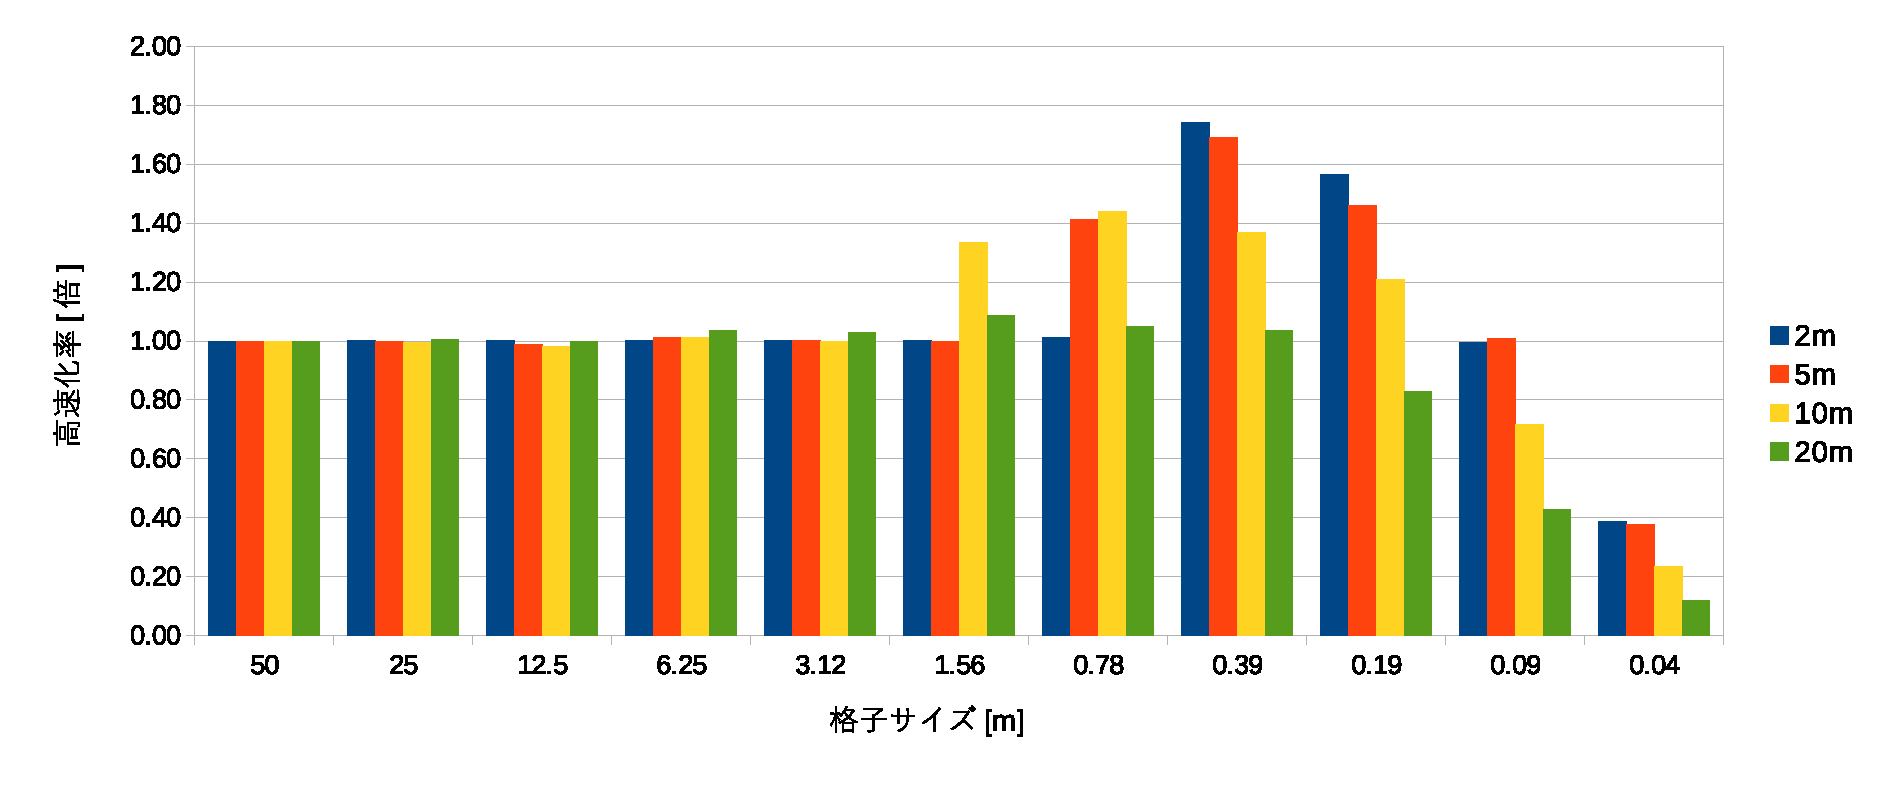
\includegraphics[width=12.5cm,clip]{figure/5_kousokukaritu.eps}
  \caption{通路幅を変えたときの高速化率}
  \label{fig:5_kousokuka_haba}
 \end{center}
\end{figure}


\begin{figure}[tb]
 \begin{center}
  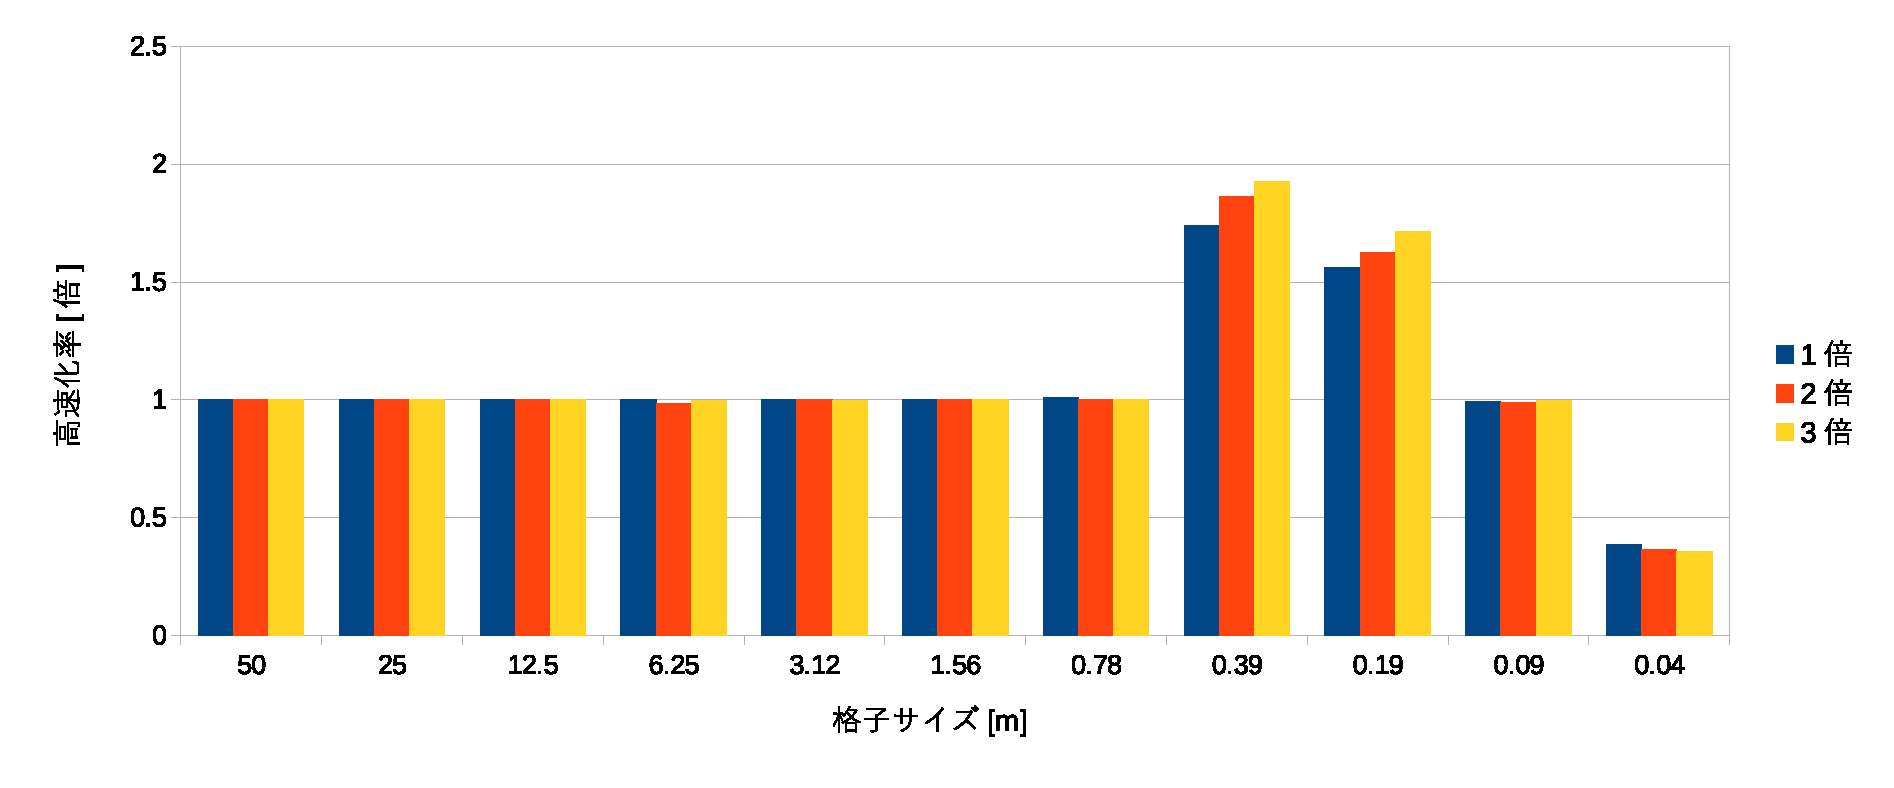
\includegraphics[width=12.5cm,clip]{figure/5_bai_kousokukaritu.eps}
  \caption{壁粒子数を変えたときの高速化率}
  \label{fig:5_kousokuka_atusa}
 \end{center}
\end{figure}


\clearpage
\subsection{シミュレーション精度の測定}
\ref{sec:5_calc_jikan}節より,
提案手法は,一部の格子サイズでセル分割法よりも高速に解析できることが確認できた.
一方で,本手法は,解析領域を格子状に分割した格子ごとに計算した進行方向ベクトル$e$と
障害物を避ける力$F_{iW}$を解析中に用いるため,セル分割法のシミュレーションと比べて
シミュレーション誤差が生じる手法となる.
このため,提案手法の格子ごとのシミュレーション結果と従来手法であるセル分割法の
シミュレーション結果を比較し,シミュレーション精度を確かめる.
誤差は,提案手法とセル分割法が算出した時間ステップごとに各エージェントの座標を
出力し,2手法の同時刻・同エージェントどうしによるエージェント間距離の最大値とする.
\textbf{
[図○○に各配置のシミュレーションの最大誤差を示す.]
}


\clearpage
\subsection{避難シミュレーションに対する提案手法の有効性}
\label{sec:5_real}
本節では,実問題に対する提案手法の有効性を示すために,実際の状況下で
避難シミュレーションを行い,シミュレーション実行時間とシミュレーション精度を
確かめる.
本評価に用いるエージェントの初期配置は,\figref{fig:kyositu_haichi},\figref{fig:pc_haichi}に示すように,大学の演習室や教室の避難時の配置で設定する.
\figref{fig:kyositu_haichi},\figref{fig:pc_haichi}の黒点は壁粒子,紫色の点はエージェント,青色の丸は経由地の座標およびゴール判定の大きさ,赤色の矢印は経由地のグラフを示す.
それぞれの配置のエージェントや壁,経由地は,\tabref{tb:haichi_para}に示すような数で配置する.
本測定では,パラメータを\tabref{tb:result_para}で設定し,すべてのエージェントが
部屋から避難できるまでを刻み値0.001で解析する.
\textbf{
[結果を表示する]
}


\begin{eqnarray}
\label{eq:gosa_hinan}
\mbox{誤差$[\%]$} = \left | \frac{C_{time} - T_{time}}{C_{time}} \right | \times 100
\end{eqnarray}

\begin{figure}[tb]
	\begin{minipage}[b]{0.5\columnwidth}
		\centering
		\includegraphics[width=\columnwidth]{figure/kyositu_v2.eps}
		\caption{教室の初期配置}
    \label{fig:kyositu_haichi}
	\end{minipage}
	\begin{minipage}[b]{0.5\columnwidth}
		\centering
		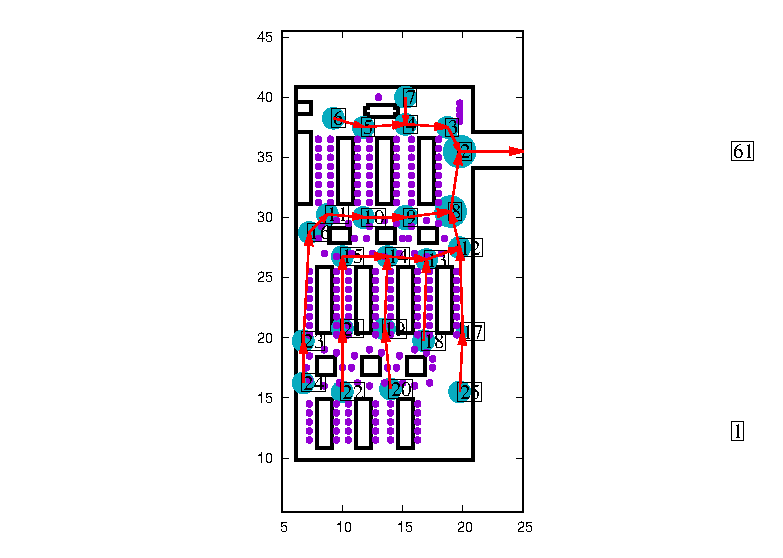
\includegraphics[width=\columnwidth]{figure/pc_m.eps}
		\caption{演習室の初期配置}
    \label{fig:pc_haichi}
	\end{minipage}
\end{figure}



\begin{table}[tb]
  \begin{center}
    \caption{各配置の詳細}
    \label{tb:haichi_para}
    \begin{tabular}{c|c|c}
      \hline \hline
      & 教室 & 演習室 \\ \hline 
      エージェント数[人] & 96 & 204 \\ \hline
      壁粒子数[個] & 1037 & 1454\\ \hline
      経由地数[個] & 12   & 26 \\ \hline
      解析領域 & $50m\times50m$ & $50m\times50m$ \\ \hline
    \end{tabular}
  \end{center}
\end{table}


%教室と演習室の解析時間{{{
\begin{figure}[tb]
	\begin{minipage}[b]{0.48\columnwidth}
		\begin{center}
		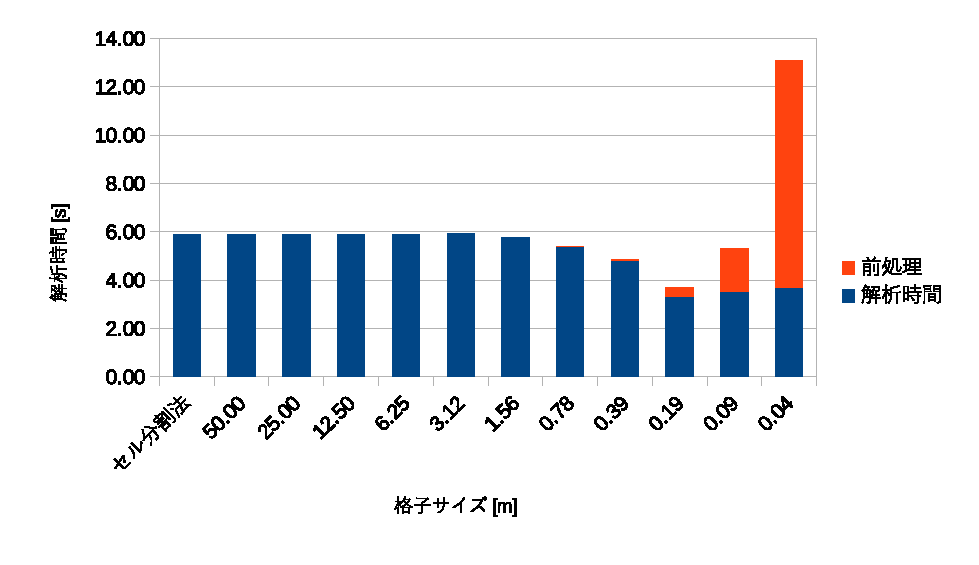
\includegraphics[width=\columnwidth]{figure/20231016_kyositu_time.eps}
		\caption{教室の配置における格子サイズごとの解析時間}
		\label{fig:kyositu_time}
		\end{center}
	\end{minipage}
	\hspace{0.04\columnwidth}
	\begin{minipage}[b]{0.48\columnwidth}
		\begin{center}
		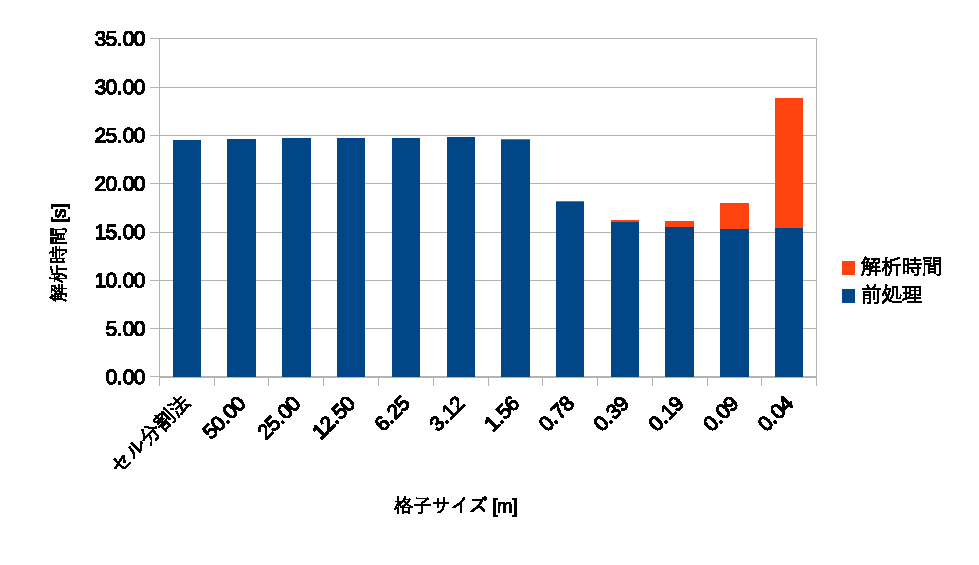
\includegraphics[width=\columnwidth]{figure/20231016_pc_time.eps}
		\caption{演習室の配置における格子サイズごとの解析時間}
		\label{fig:pc_time}
		\end{center}
	\end{minipage}
\end{figure}
%}}}

%教室と演習室の誤差{{{
\begin{figure}[tb]
	\begin{minipage}[b]{0.48\columnwidth}
		\begin{center}
		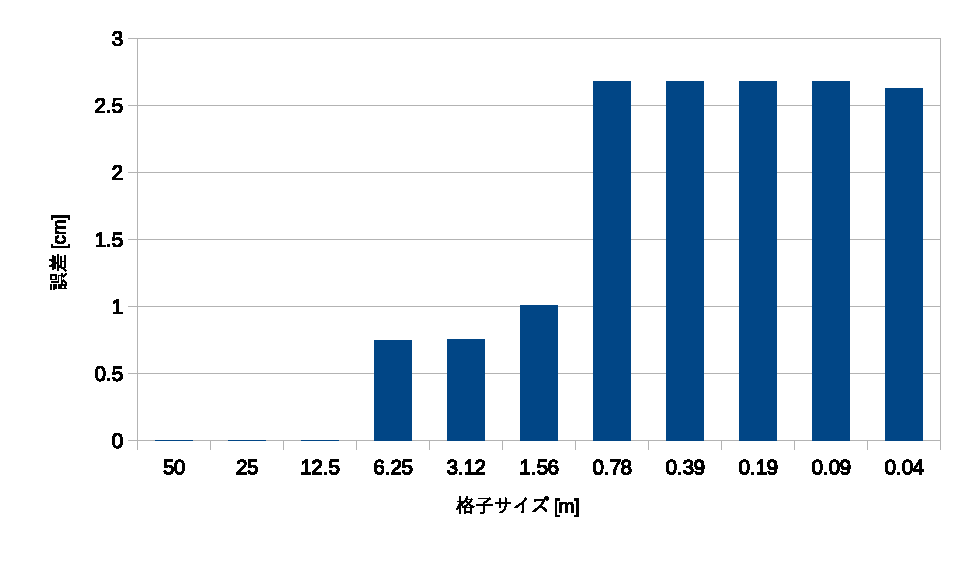
\includegraphics[width=\columnwidth]{figure/20231016_kyositu_gosa.eps}
		\caption{教室の配置における格子サイズごとの最大誤差}
		\label{fig:kyositu_gosa}
		\end{center}
	\end{minipage}
	\hspace{0.04\columnwidth}
	\begin{minipage}[b]{0.48\columnwidth}
		\begin{center}
		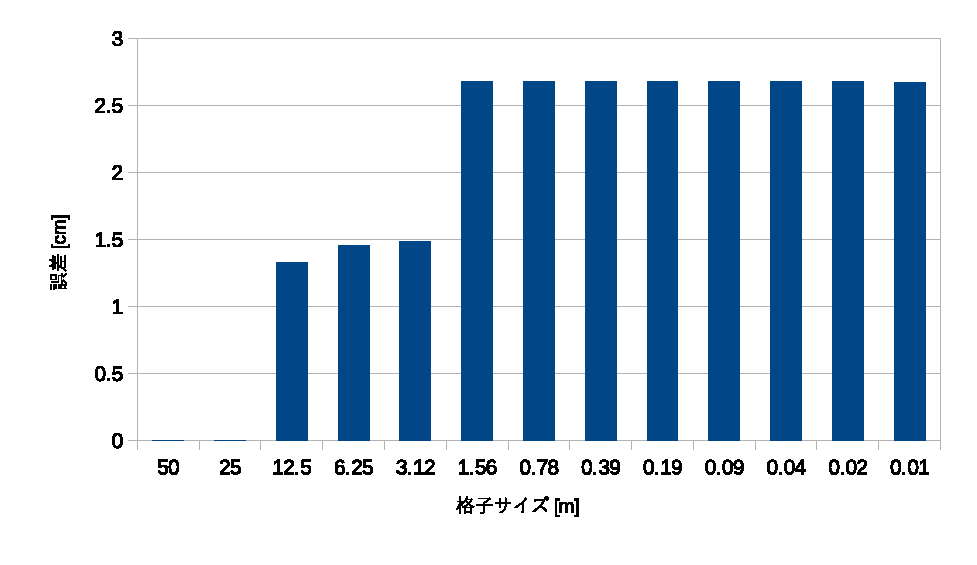
\includegraphics[width=\columnwidth]{figure/20231016_pc_gosa.eps}
		\caption{演習室の配置における格子サイズごとの最大誤差}
		\label{fig:pc_gosa}
		\end{center}
	\end{minipage}
\end{figure}
%}}}


%\figtb{格子サイズごとの解析時間(教室)}{}{8.0}{20231016_kyositu_time}{kyositu_time}
%\figtb{格子サイズごとの解析時間(演習室)}{}{8}{20231016_pc_time.eps}{pc_time}
%\figtb{格子サイズごとの最大誤差(教室)}{}{8.0}{20231016_kyositu_gosa}{kyositu_gosa}
%\figtb{格子サイズごとの最大誤差(演習室)}{}{8}{20231016_pc_gosa.eps}{kyositu_gosa}


\clearpage
\section{本章のまとめ(工事中)}
工事中.

% vim: set tabstop=4 :
%**********************************************************
\chapter{おわりに}
\label{sec:discuss}
%**********************************************************
本論文では,これまで述べてきた提案手法とその評価結果をまとめ,本研究全体の総括を行う.
本研究では,SFMを用いた人流シミュレーションを高速化するために,
エージェント間距離の計算回数削減手法と,
進行方向の計算回数削減手法を提案し,その有効性を評価した.

第\ref{sec:reduce_distance}章「エージェント間距離の計算回数削減手法」では,
視野パラメータを用いたSFMの人流シミュレーションにおいて,周囲のエージェントが
視野範囲内に存在するかの判定に必要なエージェント間距離の計算回数を削減する手法を提案した.
SFMを用いた人流シミュレーションは,一般的にセル分割法を用いることで,
エージェント間距離の計算回数の削減が行われている.
セル分割法は,影響範囲が円形であることを前提としており,視野を用いたSFMのように影響範囲が
扇形の場合を想定していない.
このため,視野を用いたSFMに一般的なSFMのエージェント間距離の計算回数削減手法を用いると,
影響範囲を円形に絞り込みをした上で,視野形状に合わせた扇形に絞り込みを行う操作が必要となる.
本提案手法では,視野形状である扇形に近似した領域を設定し,
近似領域外のエージェントに対するエージェント間距離の計算回数を削減することで,
視野を用いたSFMを高速化する.
評価の結果,提案手法は,エージェントが交差するように移動する問題において,
十分に許容可能な誤差の範囲で約1.25倍の高速化率が得られることを確認した.
%他にもあればここに追記予定


第\ref{sec:reduce_travel_direction}章「格子分割を用いた進行方向の計算回数削減手法」では,
SFMを用いた人流シミュレーションにおいて,
進行方向をあらかじめ計算することで,解析中の進行方向の計算回数を削減する手法を提案した.
本手法は,目的地や障害物の座標が解析中に変化しない特徴を利用し,解析領域を格子状に分割した
領域ごとに目的地に向かうベクトルと障害物を避ける力を計算し,解析中にその値を用いて
解析する
評価の結果,提案手法は,通路を再現した配置を移動する問題において,
エージェントの進行方向の計算回数を最大○○\%削減し,シミュレーション実行時間を
最大○○倍高速に解析できることを確認した.
また,提案手法は,避難シミュレーションにおいても,大学の施設を再現した配置から避難する様子を
再現する解析で十分に許容できる誤差の範囲で最大○○倍高速に解析できることを確認した.

\textbf{続く}


%***** END ************************************************


%------------------------------------------------------------------
% 注意点
%------------------------------------------------------------------
% 「おわりに」は,ここまでの文章をすべて読んできた人向けの文章です.
% このため,細かな用語の説明は必要ありません.
% 論文の論理構造が分かるような文章を1\UTF{FF5E}2ページ目安で書いてください.
% 
% 構成例を以下に示します.
% [1段落目]
% 従来手法の問題点とそれに対する提案手法
% [2段落目]
% 提案手法の手順
% [3]段落目以降
% 評価結果とそこから導き出される結論
%
%------------------------------------------------------------------



%====[ 謝辞 ]========================================================
\clearpage
\addcontentsline{toc}{chapter}{謝辞}
\markright{謝辞}
% vim: set tabstop=4 :
%******************************************************************
\chapter*{謝辞}
\label{sec:thanks}
%******************************************************************

本研究を進めるにあたり,ご指導いただいた中村さんに深く感謝いたします.
この感謝の気持ちを伝えるために,私は中村さんに10000円をさしあげます.




\thanksend
%************************* END ************************************


%------------------------------------------------------------------
% 謝辞例文集(これが礼儀的にどうなのかは謎.自己責任で使用すること)
%               ※指導教員の名前は必ず書くのが礼儀です.
%------------------------------------------------------------------
%
% 本研究の機会及び素晴らしい実験環境を与えて下さり,
% 貴重な時間を割いて研究の方向性を御指導頂きました○○ ○○教授に
% 深く感謝致します.
%
% 本研究を進めるにあたり,
% 日頃から惜しみなく御指導して頂きました○○ ○○氏に
% 心から感謝致します.
%
% 研究の方向性をはじめ研究の細部に至るまで数々の有意義な御意見,
% 御助言を賜わりました○○ ○○氏に
% 感謝致します.
%
% 特に,本研究のきっかけを与えて下さり,研究の進め方から文章の
% 書き方まで丁寧に御指導下さった
% ○○ ○○氏には
% この場を借りて心から深く感謝致します.
%
% 貴重な御意見,様々な御提案を頂いた××ゼミの皆様に御礼申し上げます.
%
% 最後に,私をここまで育てて下さった家族に深く感謝します.
%
%------------------------------------------------------------------


%====[ 参考文献 ]====================================================

\clearpage
\addcontentsline{toc}{chapter}{参考文献}
\markright{参考文献}
\bibliography{bibfile}          % どちらか片方を選択     
%%ここに参考文献を入力

\begin{thebibliography}{99}
\bibitem{soturon1}
	  aaaaaaaaaaaaaaaaa
  \bibitem{soturon2}
	 虞飛,佐藤裕幸: aa高解像度画像対応ステレオマッチングのGPGPUによる
	  高速化,情報処理学会研究報告,Vol.2017-HPC-160 No.19 (2017).
  \bibitem{soturon3}
	  大田弘樹,馬場明子,下田雄一,安田隆洋,山本啓二: GPGPUを用い
	  たソフトウェア高速化手法,MSS技報,Vol27 (2017).
  \bibitem{soturon4}
	  Hisa Ando:GPUを支える技術,技術評論社(2017)
  \bibitem{soturon5}
	  柳田匠,田中輝雄,藤井昭宏: GPUを用いた行列-行列積の実装と性能
	  評価,情報処理学会第81回全国大会,(2019)
  \bibitem{soturon6}
	  K.F.RILEY,M.P.HOBSON,and S.J.BENCE:Mathematical Methods for
	  physics and engineering,Cambridge University Press(2010).
  \bibitem{soturon7}
	  Cheng.J,Grossman.M,and McKercher.T.株式会社クイープ:CUDA C
	  プロフェッショナルプログラミング,インプレス(2015).
  \bibitem{soturon8}
	  NVIDIA TESLA V100 GPU ARCHITECTURE, available from<http://images.
nvidia .com/content/volta-architecture/pdf/volta-architecture-whitepaper.pdf>
	  (accessed 2020-11-16).
  \bibitem{soturon9}
	  Dissecting the NVIDIA Volta GPU Architecture via
	  Microbenchmarking,available
	  from<https://arxiv.org/pdf/1804.06826.pdf>(accessed
	  2020-11-25)
  \bibitem{soturon10}
	  Using Tensor Cores for Mixed-Precision scientific Computing,
	  available
	  from<https://developer.nvidia.com/blog/tensor-cores-mixed-precision-scientific-com
	  puting>(accessed 2020-11-20)
  \bibitem{soturon11}
	  Programming Tensor Cores in CUDA9,available
	  from<https://developer.nvidia.com/blog/programming-tensor-cores-cuda-9/>(accessed
	  2020-11-25)
	  
 \bibitem{soturonaaaaaaaa}	 
	 Kerr,A.Merril,D.Demouth,J.Tran,J:CUTLASS:Fast Linear
	 Algebra in CUDA C++,NVIDIA Developer Blog(オンライン),
	 available
	 from<https://developer.nvidia.com/blog/cutlass-linear-algebra
	 -cuda>(accessed2020-09-02).
	 
%人名,人名:研究タイトル,書籍名,Vol.数値,No.数値,pp.数値-数値(発行年).
\end{thebibliography}
                % どちらか片方を選択


%====[ 付録 ]========================================================
\appendixes             %付録に章番号が必要ない場合は"es"を削除(\appendixにする)
% vim: set tabstop=4 :
%**********************************************************
\chapter{プログラムの説明}
\label{sec:appendix}
%**********************************************************

付録には,添付するソースコードの説明を書いてください.
データ構造や主要な変数の説明は本文中で述べてあると思います.
本文で述べたことを一覧形式でまとめる分には構いませんが,
まったく同じことを書くのはよくありません.
このため,本文中では書けない実装の話
(コンパイル方法や, 測定条件の変更方法,入出力フォーマットなど)
を中心に書きましょう.


また,付録のページは,
本文中で邪魔になった定義とか証明とかの避難場所としても利用可能です.



\section{節番号のテスト}
\subsection{項番号のテスト}
付録では,こんな風に章番号が表示されます.
付録A, 付録Bというように,付録のchapterにも章番号をつけたい場合は,
main.tex66行目の$\setminus$appendixを$\setminus$appendixesに変更してください.


\section{ページレイアウト表示}
texの機能を使ってページレイアウトの情報を表示する.

\layout %論文執筆時には必ず消してね.

%***** END ************************************************

\end{document}
